%\documentclass[12pt,notitlepage]{article}
\documentclass[a4paper,12pt]{article}
\usepackage[utf8]{inputenc}
\usepackage{graphicx}
\usepackage{verbatim}
\usepackage{amsthm}
\usepackage{pdfpages}
\usepackage{amsmath}

\usepackage{mathtools}
\DeclarePairedDelimiter\ceil{\lceil}{\rceil}
\DeclarePairedDelimiter\floor{\lfloor}{\rfloor}

\usepackage{hyperref}
%\usepackage[T1]{fontenc}
\usepackage{url}
\usepackage{lipsum}
\usepackage{array}
\usepackage{multirow}
\usepackage{float}
\usepackage{lscape}
\usepackage{colortbl}
\newcolumntype{P}[1]{>{\centering\arraybackslash}p{#1}}
\usepackage[nottoc,numbib]{tocbibind}
\usepackage{fancyhdr}
\usepackage{hhline}
\usepackage[printonlyused]{acronym}

%\usepackage{txfonts}
\usepackage{lipsum,etoolbox}% http://ctan.org/pkg/{lipsum,etoolbox}
\usepackage{caption}
\usepackage{subcaption}

\usepackage{algorithm}
\usepackage[noend]{algpseudocode}

\makeatletter
\def\BState{\State\hskip-\ALG@thistlm}
\makeatother

\usepackage{minted}

\definecolor{black}{RGB}{0,0,0}

\usepackage{fancyvrb}

\usepackage{geometry}
\geometry{
	a4paper,
	total={170mm,257mm},
	right=3cm,
	left=3.5cm,
	top=3cm,
	bottom=3cm
}


\usepackage{titlesec}
\usepackage{hyperref}
\titleclass{\subsubsubsection}{straight}[\subsection]

\newcounter{subsubsubsection}[subsubsection]
\renewcommand\thesubsubsubsection{\thesubsubsection.\arabic{subsubsubsection}}
\renewcommand\theparagraph{\thesubsubsubsection.\arabic{paragraph}} % optional; useful if paragraphs are to be numbered

\titleformat{\subsubsubsection}
{\normalfont\normalsize\bfseries}{\thesubsubsubsection}{1em}{}
\titlespacing*{\subsubsubsection}
{0pt}{3.25ex plus 1ex minus .2ex}{1.5ex plus .2ex}

\makeatletter
\renewcommand\paragraph{\@startsection{paragraph}{5}{\z@}%
	{3.25ex \@plus1ex \@minus.2ex}%
	{-1em}%
	{\normalfont\normalsize\bfseries}}
\renewcommand\subparagraph{\@startsection{subparagraph}{6}{\parindent}%
	{3.25ex \@plus1ex \@minus .2ex}%
	{-1em}%
	{\normalfont\normalsize\bfseries}}
\def\toclevel@subsubsubsection{4}
\def\toclevel@paragraph{5}
\def\toclevel@paragraph{6}
\def\l@subsubsubsection{\@dottedtocline{4}{7em}{4em}}
\def\l@paragraph{\@dottedtocline{5}{10em}{5em}}
\def\l@subparagraph{\@dottedtocline{6}{14em}{6em}}
\makeatother

\setcounter{secnumdepth}{4}
\setcounter{tocdepth}{4}

\begin{document}
	\begin{titlepage}
		\begin{center}
			\includegraphics[width = \textwidth]{logo_ntu_new.png}
			\vspace*{3cm}
			
			\Large
			\textbf{Decentralised Content Trust for Docker Images in Data Centers}\\		
			\vspace{1.2cm}
			\textbf{By\\ Brandon Goh Wen Heng}\\
			 Agency for Science, Technology and Research (A$^\star$STAR), Data Storage Institute (DSI)\\\vspace{1.2cm}July 2017\\\vspace{1.2cm}
			Final Report Submitted in Partial Fulfillment of the \\Honours Requirements for the Degree of\\Mathematical Sciences.
		
			\vspace{1.2cm}
			Division of Mathematical Sciences\\
			School of Physical and Mathematical Sciences\\
			Nanyang Technological University\\
			\vfill
		\end{center}
	\end{titlepage}

\pagenumbering{roman}

	\tableofcontents
	\newpage
\phantomsection
\addcontentsline{toc}{section}{Abstract}
\section*{Abstract}
{\par \noindent This report is to present research that has been completed during the 12 weeks of internship at A$^\star$STAR. Chapter 1 will focus on the background and the objectives of research set forth for this internship. Chapter 2 will introduce broad concepts on Docker and blockchains, which are fundamental in understanding the following chapter. Completed research will be presented in detail in chapter 3, in the following order. Bitcoin and Docker will be touched on briefly, followed by the integration of these two technologies. Following will be an introduction to Ethereum and architecture and protocols that are shared by both cryptocurrencies. Chapter 4 will end the report by detailing the expected direction of future research moving forward.}
\newpage

\phantomsection
%	\addcontentsline{toc}{section}{List of Tables}
\listoftables
\newpage

\phantomsection
%	\addcontentsline{toc}{section}{List of Figures}
\listoffigures
\newpage
	\phantomsection
\addcontentsline{toc}{section}{List of Abbreviations}
\section*{List of Abbreviations}
	\begin{acronym}[OPCODE]
		\acro{AMD}{Advanced Micro Devices}
		\acro{API}{Application Programming Interface}
		\acro{ARM}{Advanced \ac{RISC} Machine}
		\acro{AVX}{Advanced Vector Extensions}
		\acro{ASIC}{Application-Specific Integration Circuit}
		\acro{AUFS}{Advanced Multi-Layered Union Filesystem}
		\acro{AWS}{Amazon Web Services}
		\acro{CPU}{Central Processing Unit}
		\acro{DAG}{Directed Acyclic Graph}
		\acro{DDoS}{Distributed Denial of Service}
		\acro{DDT}{Decentralised Docker Trust}
		\acro{DHT}{Distributed Hash Table}
		\acro{DoS}{Denial of Service}
		\acro{ECDSA}{Elliptic Curve Digital Signature Algorithm}
		\acro{FPGA}{Field-Programmable Gate Array}
		\acro{FQDN}{Fully Qualified Domain Name}
		\acro{GBT}{GetBlockTemplate}
		\acro{GHOST}{Greedy Heaviest-Observed Sub-Tree}
		\acro{GPU}{Graphics Processing Unit}
		\acro{GUI}{Graphical User Interface}
		\acro{HMAC}{Hash Message Authentication Code}
		\acro{IoT}{Internet of Things}
		\acro{I/O}{Input/Output}
		\acro{KDF}{Key Derivation Function}
		\acro{LES}{Light Ethereum Subprotocol}
		\acro{OPCODE}{Operation Code}
		\acro{OS}{Operating System}
		\acro{PKI}{Public Key Infrastructure}
		\acro{RAM}{Random Access Memory}
		\acro{REST}{Representational State Transfer}
		\acro{RISC}{Reduced Instruction Set Computing}
		\acro{RLP}{Recursive Length Prefix}
		\acro{RPC}{Remote Procedure Call}
		\acro{SIMD}{Simple Instruction, Multiple Data}
		\acro{SPV}{Simplified Payment Verification}
		\acro{SSE}{Streaming \ac{SIMD} Extensions}
		\acro{TCP}{Transmission Control Protocol}
		\acro{TUF}{The Update Framework}
		\acro{VM}{Virtual Machine}
	\end{acronym}
	
	\newpage
\pagenumbering{arabic}
	\pagestyle{plain}{%
		\fancyhf{}%
		\fancyfoot[C]{\thepage}%
		\renewcommand{\headrulewidth}{0pt}%
		\renewcommand{\footrulewidth}{0pt}%
	}
	\section{Research Topic}
	
	\subsection{Background \& Motivation}
	{\par Linux containers are quickly gaining traction as a new way of building, deploying, and managing applications in the cloud-enabled data center. Containers couple lightweight, high-performance isolation with security and make it easy to package services and deploy them in a flexible and scalable way. \\\newline Over the past decade, hypervisor-based virtualization has become a dominant data center technology.
		The concept is simple: create a virtual implementation of the hardware of a physical computer so that it can run an entire, unmodified operating system within it. The result, a virtual machine monitor, provided a powerful tool through which to consolidate multiple servers and take better advantage of additional physical computing resources.\\
		\newline
		Hypervisors, however, introduce additional workload-dependent overhead as they faithfully replicate true hardware behaviors. In addition, hypervisors also bring portability considerations as to where the application(s) can run: on premises, public cloud, private cloud, bare metal, mixed environment, etc.\\\newline
	Blockchain technology is also gaining attention with Bitcoin and Ethereum being the two most popular frameworks that are powered by blockchain. Apart from the traditional use of transferring cryptocurrencies among blockchain participants, smart contracts and data can be stored and run from the blockchain.\\\newline
The properties of immutability, anonymity and transparency provides assurances that data cannot be altered by any means while preserving user confidentiality. This is further strengthened by the use of strong cryptography where authentication is done using private keys that only the owner is aware of. This is in contrast to traditional systems where users can easily be identified by their usernames.\\\newline
However, blockchains suffer from performance and network bottlenecks when blockchains grow too large.}
	\subsection{Research Objectives}
	{\par The first focus of this research is the use of system containers. That is, containers which offer an environment as close to possible as the one from a \ac{VM} but without the overhead that comes with running a separate kernel and simulating all the hardware.\\\newline The second focus is the use of the blockchain networks. That is, studying of the architecture of the blockchain and its supported uses that could facilitate movement of information beyond transfer of currencies.}
	\pagenumbering{arabic}
	\newpage
	\section{Introduction}
	\subsection{Docker}
	{\par Docker is an open-source platform for rapid development and deployment of applications within containers. Similar to a \ac{VM}, software running within the containers are isolated from other containers and the underlying host \ac{OS} \cite{DockerSec}. \\
		\newline
		Docker includes additional features, such as its \textit{swarm} technology, which allows emulation of a server cluster through the provisioning of multiple containers from the same image. Using this technology, we can perform horizontal scaling quickly by tweaking some configuration values and implementing the changes in place of the applications that are currently running, without requiring existing containers to be taken offline and re-configured. The \textit{swarm} will evenly distribute the workload across all applications with the same functionality, essentially performing the same function as a load balancer but now handled transparently by Docker Engine. Potential functions  of \textit{Docker swarm} could include  geo-replication, where data could be replicated to different regions globally, allowing quicker access to data or it could also be used to provision a failover cluster for mission-critical applications to depend on. \\
		\newline
		Docker uses a \textit{union filesystem}, which allows directories from the container and the image to be ``combined'' and presented to the application as a single directory through the container's mount point. Using this filesystem allows each container's read-write operations to be isolated within its own container, eliminating effort required in re-imaging an entire system for each application as seen on \ac{VM}s. It additionally reduces the \ac{I/O} load on the system as versioning of files is not required. Docker defaults to the use of 2 storage drivers, the first being \ac{AUFS} (Figure \ref{fig:aufs}) and the other being \textit{OverlayFS} (Figure \ref{fig:overlayfs}).	
	\begin{figure}[H]
		\centering
		\includegraphics[width=0.8\linewidth]{AUFS.eps}
		\caption[AUFS]{\ac{AUFS}}
		\label{fig:aufs}
	\end{figure}
	\begin{figure}[H]
		\centering
		\includegraphics[width=0.8\linewidth]{OverlayFS}
		\caption{OverlayFS}
		\label{fig:overlayfs}
	\end{figure}
	
	
	\iffalse
	\begin{figure}
		\centering
		\begin{subfigure}[b]{0.49\textwidth}
			\includegraphics[width=\textwidth]{AUFS}
			\caption{Advanced Multi-Layered Union Filesystem}
			\label{fig:aufs}
		\end{subfigure}
		\vline
		\begin{subfigure}[b]{0.49\textwidth}
			\includegraphics[width=\textwidth]{OverlayFS}
			\caption{OverlayFS}
			\label{fig:overlayfs}
		\end{subfigure}
		\caption{Docker Storage Drivers}\label{fig:stordrv}
	\end{figure}
	\fi
	
	\subsection{The Update Framework (TUF)}
	{\par
		Current Linux software updaters provide little to no security when connecting to repositories to obtain information on software updates. This exposes the client to eleven types of attacks \cite{PkgMgmtSec,ProtectCommunityRepo,KeyCompromiseSoftwareUpdater,DCTDocker}. \ac{TUF} helps to prevent these attacks by acting as a middle person between the client (software updater) and the repository by employing a comprehensive check of the metadata from multiple files. The metadata contains important information such as the key role, version, validity, cryptographic library used, signature hash and key ID. Specific role metadata files will contain additional information, all these is to ensure that the previous exploits cannot be easily replicated under \ac{TUF}. \ac{TUF} requires a closed \ac{PKI} where keys can only be derived and used within the architecture. It is also recommended to store the private keys of the root, target, snapshot and any other delegation roles offline or in an encrypted medium.
		\\
		\newline
		A typical repository architecture integrating \ac{TUF} consists of 5 roles:
		\begin{enumerate}\setlength\itemsep{0pt}
			\item Root, which authorises all keys used within the repository
			\item Target, which signs a metadata file containing the (relative) path of all files in the repository or it will contain the list of delegation and (relative) path of all files under each delegation (subfolders of storage root)
			\item Snapshot, which signs a metadata file containing information on all metadata files in the repository (except for Timestamp role)
			\item Timestamp, which timestamps a file containing information on the latest versions of files, the hash and file size of the snapshot file
			\item Mirrors, which contain information on mirrors that the client can choose from when updating software.
		\end{enumerate}
	}
	
	\begin{figure}[H]
		\centering
		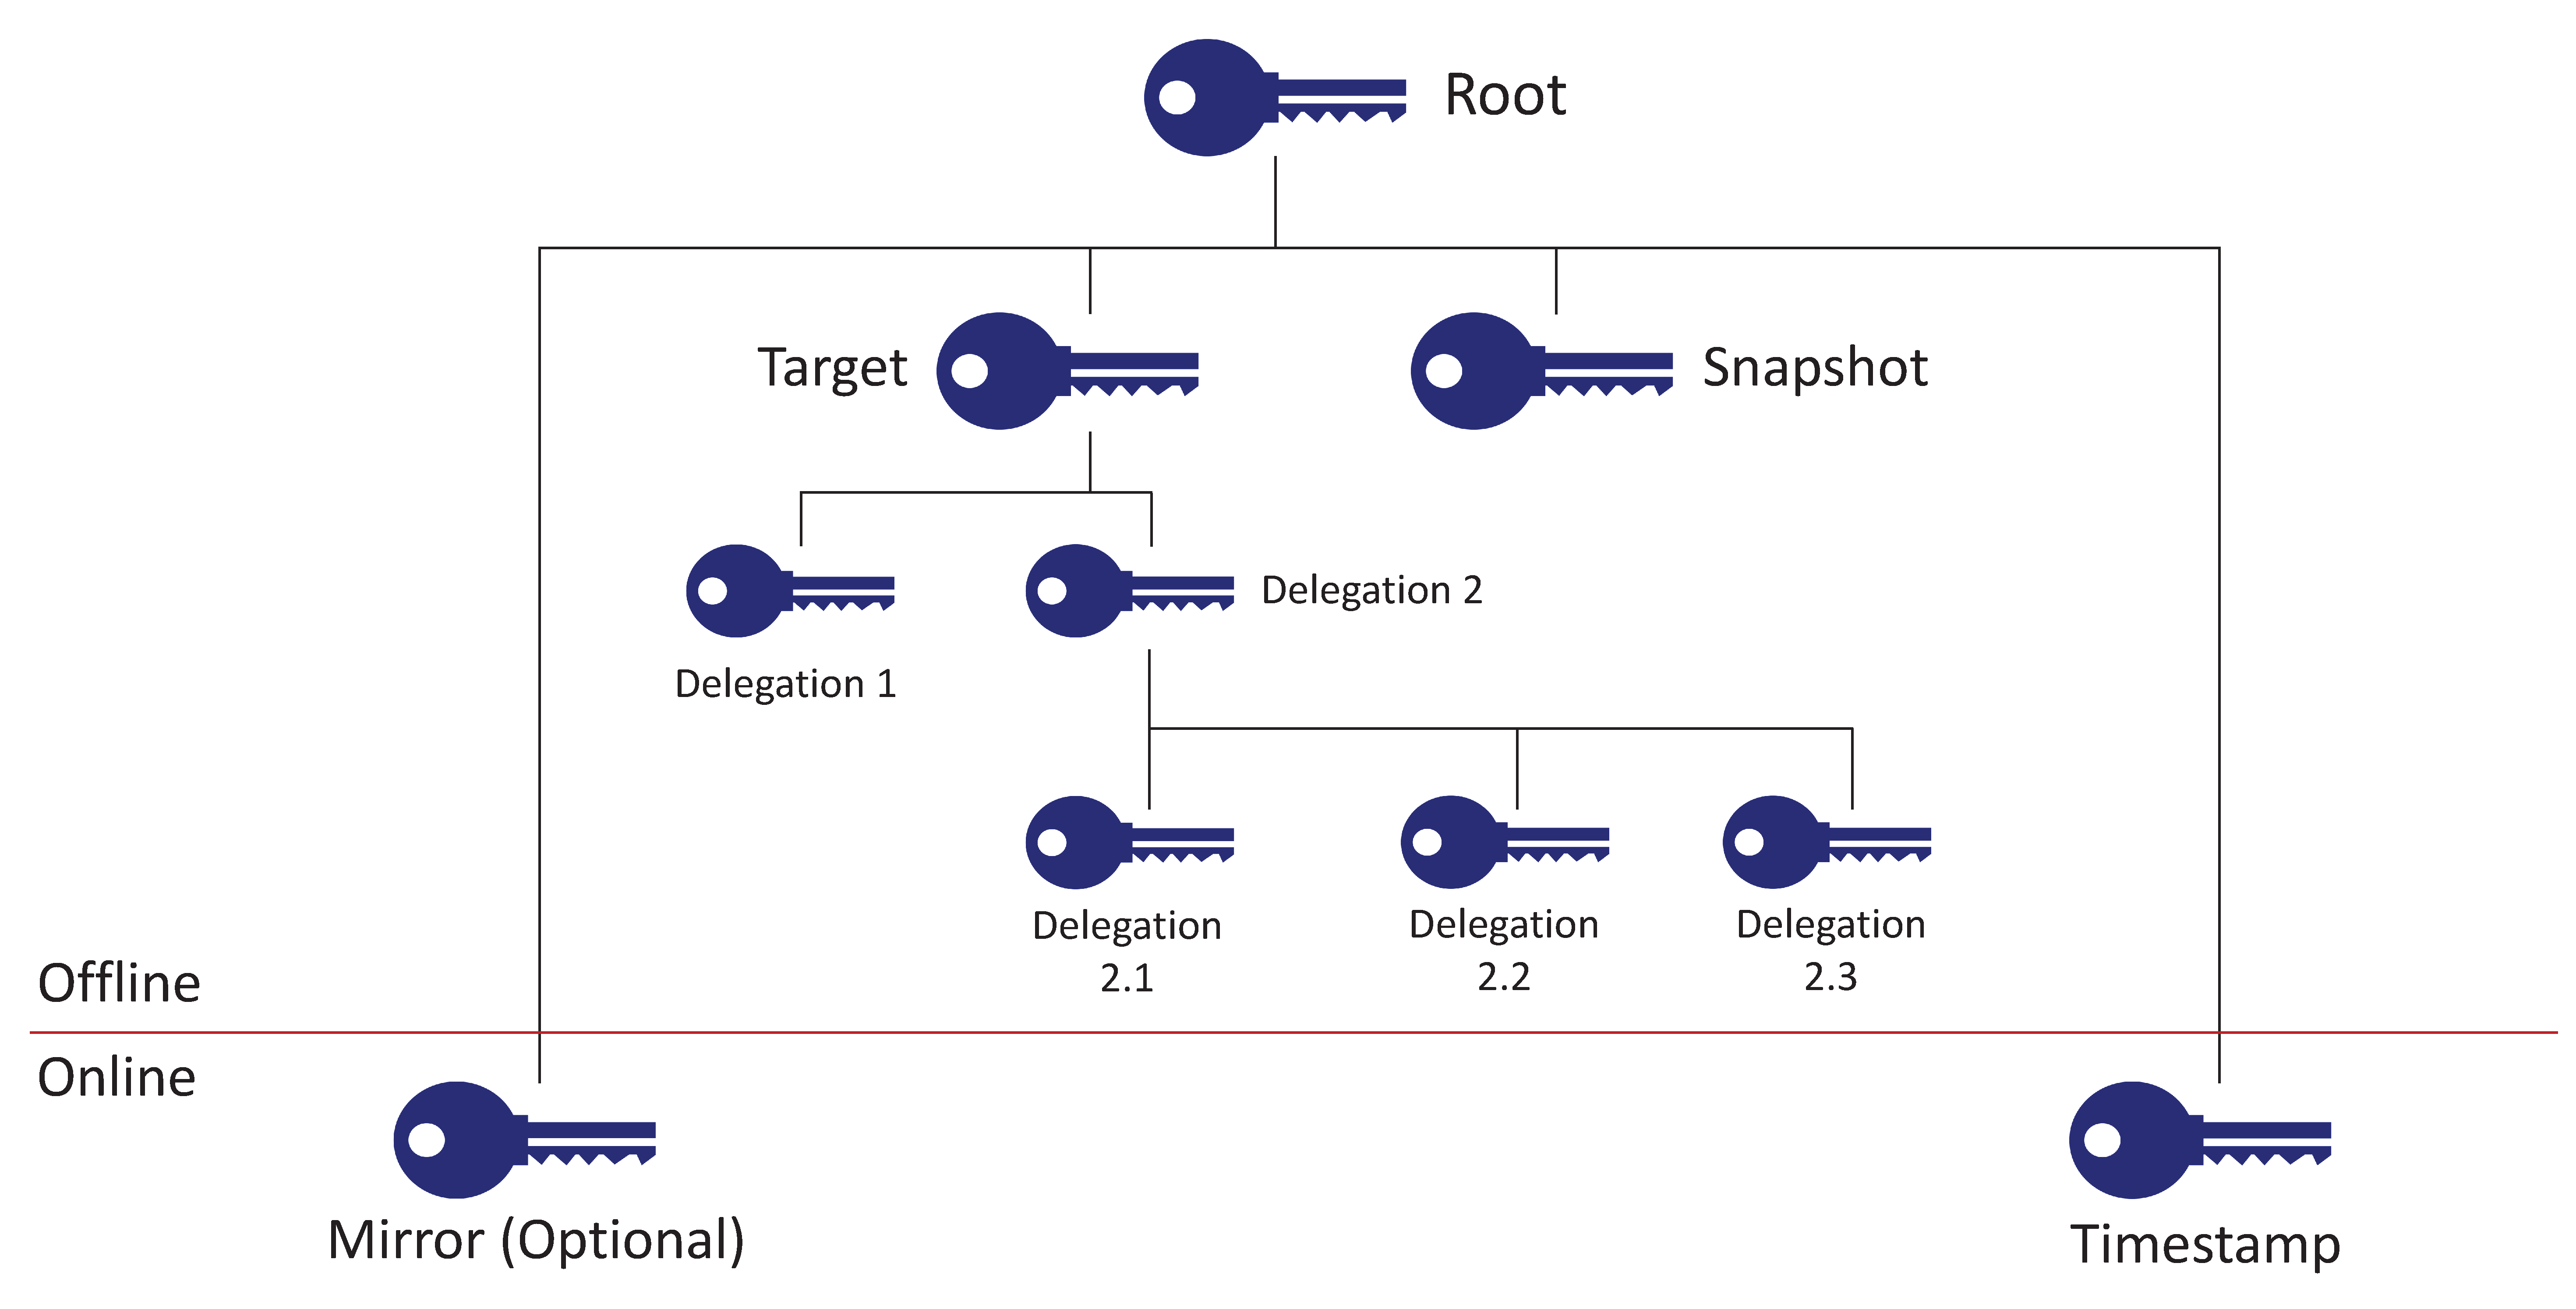
\includegraphics[width=0.7\linewidth]{TUFarc}
		\caption[TUF Architecture]{\ac{TUF} Architecture}
		\label{fig:tufarc}
	\end{figure}
	\subsection{Blockchain}
	{\par \noindent A blockchain is a distributed database which stores information in the form of \textit{blocks}. Each block includes a timestamp, a hash of the previous block and a hash of all the data in the current block, which significantly increases the difficulty of altering an existing transaction in a previous block. Increasingly,  blockchains have been found to be suitable as alternative storage mediums for important records such as medical records \cite{medrec} and identity management \cite{idenmgmtdhs,idenmgmtmsft}.
		\\
		\newline 
		Blockchains grow in size due to the continuous adding of blocks in a process known as \textit{mining}. This process will be looked at and explained in greater detail in section \ref{mining}.
		\\\newline
	There are loopholes in the blockchain that leave it exposed to attackers, most notably those who have the intention of altering records to their own benefit will require massive amounts of computing power to create a ``fork'' in the blockchain and mine blocks fast enough to satisfy the ``\textit{longest chain rule}'', with the ultimate goal of tricking users into accepting that the chain formed by the hacker is genuine. This attack is known as \textit{Double-spending}. This can be mitigated by requiring $x$ confirmations, or $x$ new blocks to be added on top of the transaction as it is assumed that the attacker is unlikely to have a hashrate exceeding 10\% of the mining network and will not have enough computing power available to significantly alter the blockchain.
		\\\newline
		Other types of attack against a blockchain include the $51\%$ attack. The $51\%$ attack involves an attacker having more than half of the entire network's hashrate. An attack of this form has a guaranteed $100\%$ success rate. Similar to the \textit{Double-spending} attack, there is a low probability of obtaining anywhere close to $10\%$ of the entire network's hashrate. Instead, exploitation of a mining pool (Section \ref{poolmine}) creates a higher probability of the attack to happen and instances of mining pools exceeding $51\%$ of the total network hashrate have previously occurred \cite{51}, causing panic within the cryptocurrency community.
		\\\newline
	}
	\section{Research Completed}
	\subsection{Bitcoin}
	{\par Bitcoin is the first successful implementation of blockchain technology and decentralised cryptocurrency which was introduced in 2009 through a programmer using the psuedonym Satoshi Nakamoto. With this system, payments can be facilitated between parties using wallet addresses, which are encoded in a 160-bit hash that cannot be easily identified or traced to the owner. Even without a system of trust, transactions can still take place with full transparency despite being completely anonymous \cite{Bitcoinimplement}. The \ac{GUI} for Bitcoin was simple and allowed for basic transactions such as creation of multiple digital wallets for separation of identities and transferring of funds within the system. \\\newline Technical specifications further detailed the use of the OP\_RETURN argument, which allowed for the storage of 80 bytes of arbitrary data within the transaction field of a block \cite{opreturn}. One example exploiting this feature is the storage of hashes that can be used to verify the integrity of the image, which will be further explained in detail in section \ref{sect:ddt} on Decentralised Docker Trust.
	}
	\subsection{Docker Notary}
	{\par Docker Notary is a service used for publishing and managing trusted repositories of content. All files that are uploaded and contained in Notary must be digitally signed to ensure the source and integrity of content can be verified by other users. With this system, anyone can provide trust over arbitrary data. Notary makes use of \ac{TUF} to provide the underlying security features while Notary handles the creation, management and distribution of metadata to preserve the integrity of the stored content.
		\\\newline The steps to installing a Notary server service can be found in Appendix A, with comments included for explanation of code.
	\subsubsection{Performance Evaluation}
	{\par \noindent In this experiment, we test the resilience of the Notary server against a \ac{DoS} attack. A \ac{DoS} attack includes the use of powerful hardware by an attacker to flood and overwhelm the network of the resource to the point where the affected system is unable to accept and process requests from legitimate sources (Figure \ref{fig:ddos}).}
	
	\begin{figure}[H]
		\centering
		\includegraphics[width=0.7\linewidth]{ddos}
		\caption{Simulating a DoS attack}
		\label{fig:ddos}
	\end{figure}
	
	{\par \noindent To efficiently generate load from a multi-core CPU system, \textit{wrk} was chosen as the benchmark uses a multithreaded design and fits the objective of the evaluation. In the setup, a Docker image of \textit{wrk} was obtained from the Docker Hub repository \textit{williamyeh/wrk} and used. Three systems were set up to emulate the client, attacker and a Notary server (Figure \ref{fig:attack-setup}). For the client, we set it up in two locations, Tokyo (Japan) and North Virginia (America). The attacker and the server were located in Singapore. As we are unable to ascertain the specific configurations for each of the systems, we provisioned based on current industry standards.}
	\begin{figure}[H]
		\centering
		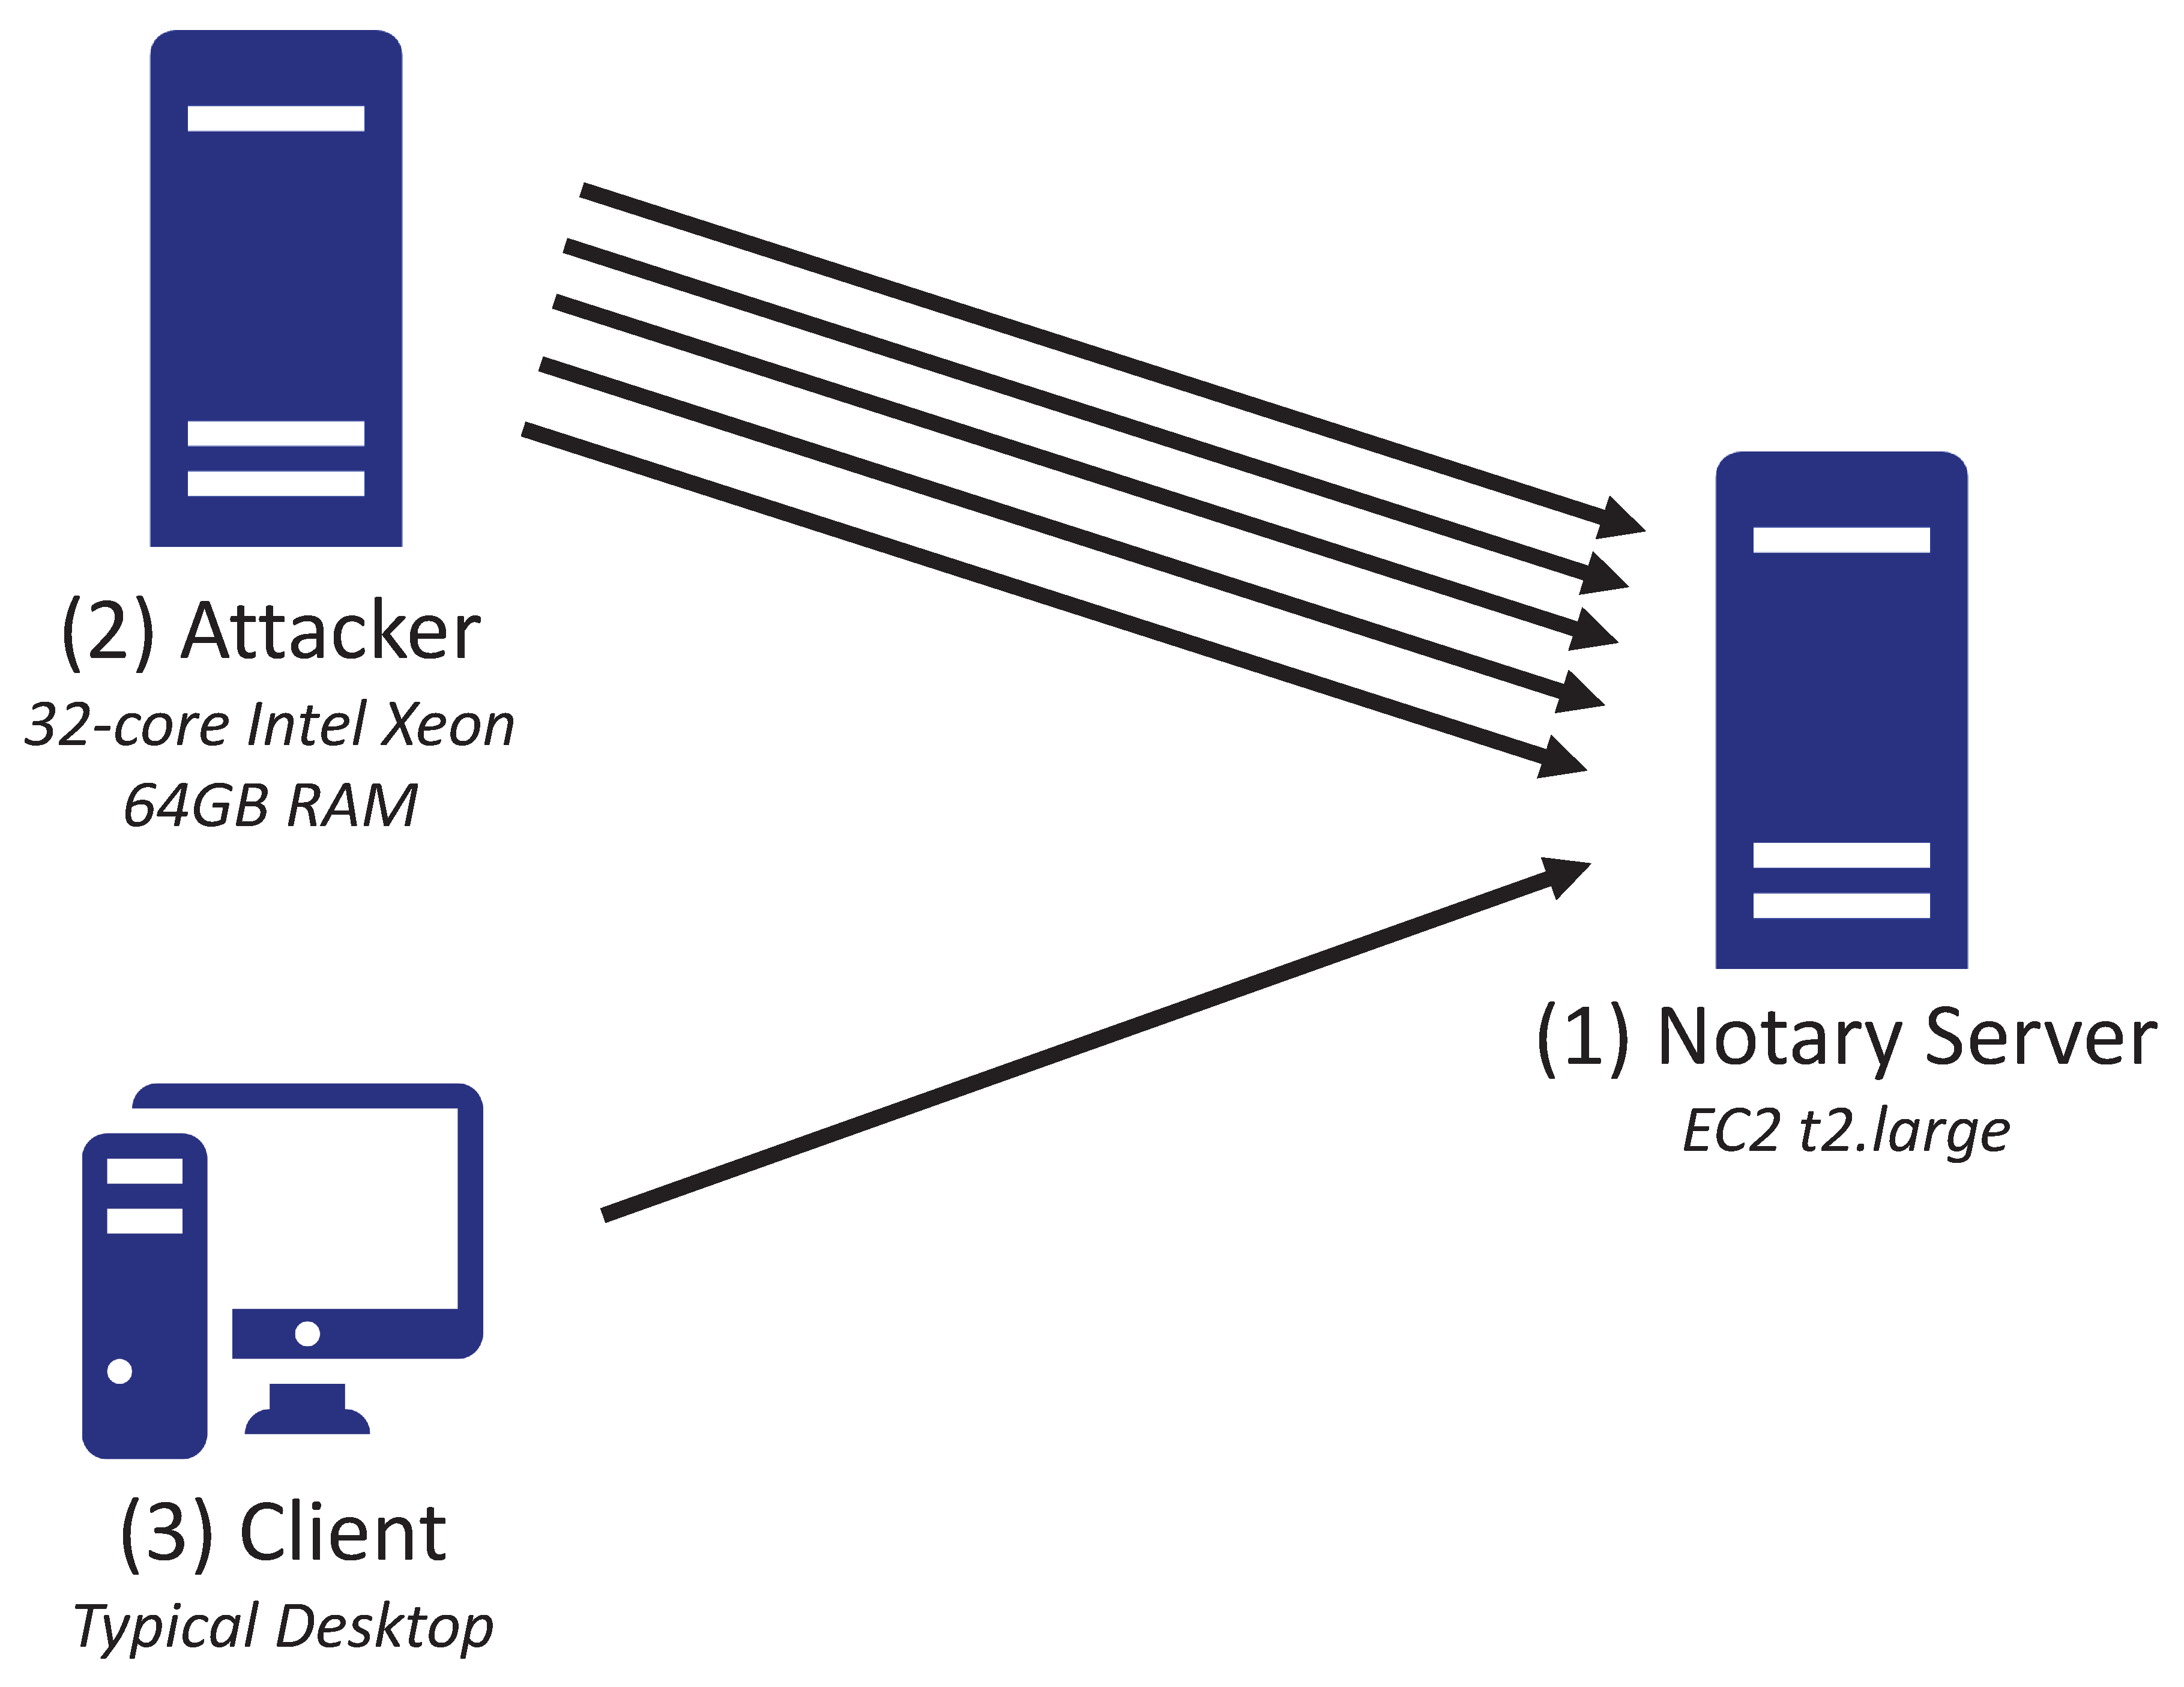
\includegraphics[width=0.6\linewidth]{attacksetup}
		\caption{Attack setup}
		\label{fig:attack-setup}
	\end{figure}
	{\par \noindent \ac{AWS} was used due to ease of setting up the systems across different geographical regions with minimal configurations and time required. The only limitation was that network bandwidth of \ac{VM}s in \ac{AWS} cannot be controlled. \\\newline The configuration for each of the systems are as follows:}
	\begin{enumerate}
		\item \textbf{Server:}\\
		We used \textit{t2.large} as it has enough resources to support a typical server setup – 2-core Intel Xeon E5-2670 @ 2.60GHz CPU and 2GB RAM. It runs Ubuntu 16.04 LTS with docker and a clean install of Notary server and MySQL.
		\item \textbf{Attacker:}\\
		We used \textit{c3.8xlarge}, consisting of a 32-core Intel Xeon E5-2680V2 @ 2.80GHz and 64GB RAM to simulate an attack with powerful hardware. It runs Arch Linux with Docker installed for running \textit{wrk}.
		\item \textbf{Client:}\\
		A \textit{t2.small} instance running 1-core Intel Xeon E5-2670 @ 2.60GHz CPU with 2GB RAM was used to emulate a typical desktop PC that runs on limited resources. Docker is installed for running \textit{wrk}.
	\end{enumerate}
}
\subsubsection{Procedure}
To perform the experiment, we vary the number of connections sent from the attacker's server to the Notary server. The client is then configured to open a single connection to the server and the number of successful requests is then recorded from the client. The steps are as follows:
\begin{enumerate}
	\item Run \textit{wrk} on the attacking server with $x$ number of connections for 2 minutes. This is to allow the Notary server to be fully saturated with connections before commencing the tests from the client side.
	\begin{Verbatim}[commandchars=\\\{\}]
docker run --rm -it williamyeh/wrk -t24 -c\(x\) -d2m --header
"Cache-Control: no-cache, no-store, must-revalidate" --header 
"Pragma: no-cache" --header "Expires: 0" https://<server FQDN>
:4443/v2/test/collection/_trust/tuf/snapshot.json
	\end{Verbatim}
	\item After about 30 seconds, we run \textit{wrk} on the client with 1 connection for 60 seconds.
	\begin{verbatim}
	docker run --rm -it williamyeh/wrk -t1 -c1 -d60s --header 
	"Cache-Control: no-cache, must-revalidate" --header "Pragma: 
	no-cache" --header "Expires: 0" https://<server FQDN>:4443/
	v2/repository/collection/_trust/tuf/snapshot.json
	\end{verbatim}
	\item Obtain the number of requests per second output from \textit{wrk} on the client server.
	\item This procedure was repeated for different values of $x$ for 5 runs each. The recorded output from these runs were recorded and averaged to minimise errors.
\end{enumerate}
\subsubsection{Results}
\label{dosresult}
The recorded results (Appendix B) from both the Japan and America region, which have been visualised in Figure \ref{fig:t2smalljapavg} \& \ref{fig:t2smallamavg}, have led us to conclude that an increase in the number of connections leads to an exponential decline in the number of successful requests made by the client. It can be further noted that eventually all requests will fail when the notary server receives concurrent connections exceeding 32000.
\begin{figure}[H]
	\centering
	\includegraphics[width=0.7\linewidth]{t2smalljapavg.eps}
	\caption{Average number of successful requests (Japan)}
	\label{fig:t2smalljapavg}
\end{figure}
\begin{figure}[H]
	\centering
	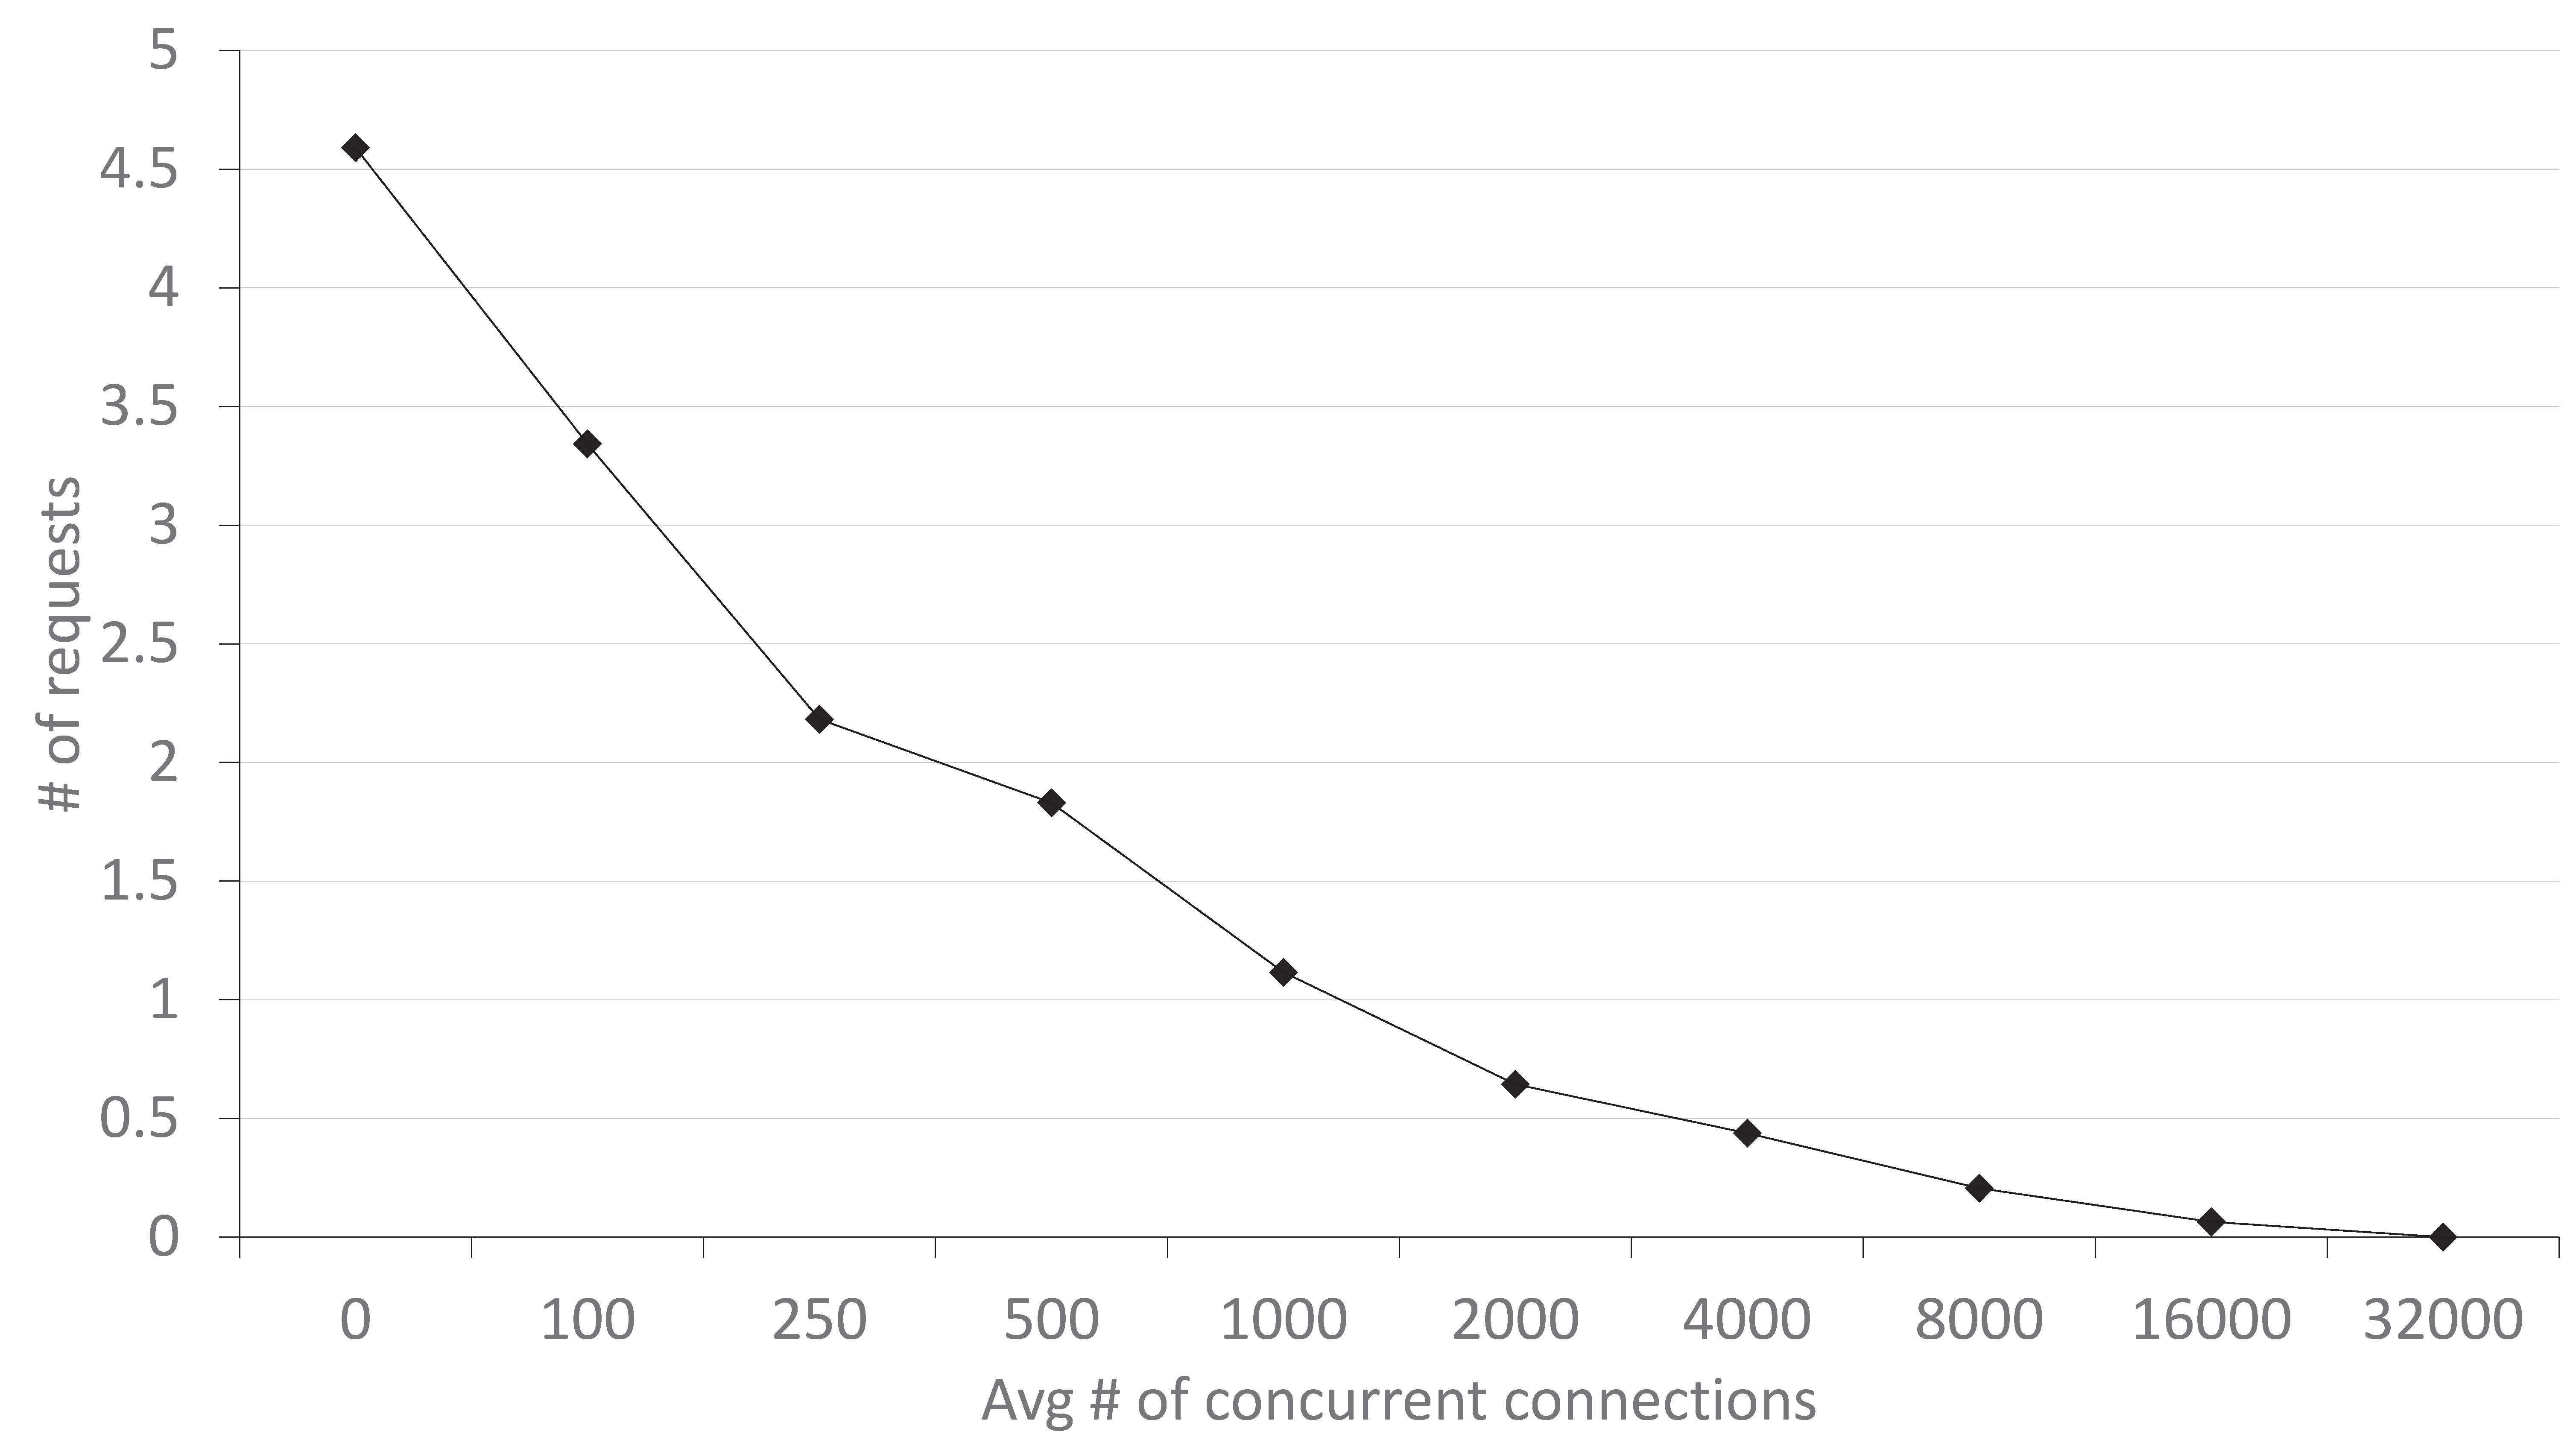
\includegraphics[width=0.7\linewidth]{t2smallamavg.eps}
	\caption{Average number of successful requests (America)}
	\label{fig:t2smallamavg}
\end{figure}
\noindent
This experiment demonstrates that a typical server setup has the capability of performing a \ac{DoS} attack. However, it must be noted that there may be occasions where requests made by the client could still be successful.

	\subsection{Decentralised Docker Trust (DDT) Framework}
	Previously seen in Section \ref{dosresult}, a \ac{DoS} attack with a simple hardware setup can easily bring down a single notary server. This provides us with motivation to finding a solution to mitigate or completely circumvent such attacks. One of the methods is to use a distributed solution (Figure \ref{fig:decentralised}).
	
\begin{figure}[H]
	\centering
	\includegraphics[width=0.7\linewidth]{decentralised}
	\caption{Distributed systems}
	\label{fig:decentralised}
\end{figure}
\noindent
	Using Bitcoin's blockchain, each node is connected to at least one other node and will have an exact copy of the blockchain \cite{blockchaindup}. This implies that if any node goes down, the system will continue to function \cite{decentralised}. This is ideal for storing critical information since it is always available. For a distributed network of a large scale to go down, an attacker will require large amounts of computing power to crash all the nodes, which is becoming increasingly impossible as it has been shown that the computing power of the Bitcoin network is 8 times more than the fastest 500 supercomputers combined \cite{compower}.\\\newline
	The \ac{DDT} framework consists of three programs designed to integrate the features of the blockchain (distributed system) and Docker (image integrity), namely Blockchain Parser, Carbonchain and the \ac{DDT} framework. The general \ac{DDT} framework can be simplified into the following image referenced by Figure \ref{fig:ddt}. These programs were created by Faruq Rasid, written in Go (or golang) and hosted on Github \cite{githubblockchain}.
	
		\begin{figure}[H]
		\centering
		
\includegraphics[width=1\linewidth]{DDT.eps}
		\caption{Decentralised Docker Trust}
		\label{fig:ddt}
	\end{figure}
	
		\subsubsection{Blockchain Parser}
	Blockchain Parser is a program primarily built for reading, verifying and writing valid blocks to and from the Bitcoin blockchain. Blockchain Parser exposes the methods for other programs such as Carbonchain to use the blockchain as these programs are unable to directly interface with the blockchain. The block architecture for Bitcoin can be referenced from Table \ref{blockstruct} in Appendix C.
	\subsubsection{Carbonchain}
	{\par Carbonchain was created as an extension to Blockchain Parser, for reading of stored data within the \textit{transaction out} field of the block and to store this output in BoltDB (Key-value pair database) as well as to create data packets which will eventually be stored in blocks and propagated into the blockchain.\\\newline
	For Carbonchain to read the data, it will first make use of Blockchain Parser for parsing the block data. Following which, Carbonchain will parse the \textit{transaction out} field and check if the packet is properly formed by looking for the \ac{OPCODE} hexadecimal \texttt{0x6a} and verifying if the size of the data is more than $20$ bytes. If both conditions are satisfied, the payload is read out from the \textit{data} field of the packet and stored in a database. After all data is extracted and concatenated (if the data was split before propagation in the blockchain), it is stored in BoltDB while the raw packets are made available to the \ac{DDT} framework for further action. The structure of the packet can be referenced from Table \ref{pktstruct} in Appendix D.\\\newline
	For Carbonchain to write the data, it must apply modifications to the payload by splitting it into blocks of $60$ bytes (if size of data exceeds $60$ bytes). It will create the necessary headers of the packet before storing the payload inside the \textit{data} field in the packet. It will append the data with the \ac{OPCODE} hexadecimal 0x6a before passing the data to Blockchain Parser. Blockchain Parser will take the formed packet, mine it into a transaction and complete the proof of work required for the block to propagate into the blockchain.
}
	\subsubsection[Decentralised Docker Trust]{Decentralised Docker Trust}
	\label{sect:ddt}
	{\par \noindent
	Docker is unable to directly interface with the blockchain as it cannot directly use Bitcoin's \ac{RPC} \ac{API}. Instead, \ac{DDT} provides an alternative way of performing operations using the \ac{REST} \ac{API}. The following paragraphs detail the processes for some commands supported by \ac{DDT}.\\\newline
\noindent
	To verify the integrity of image data using the data stored in the blockchain, the metadata from the docker image is manually extracted using the command \texttt{docker inspect} and used to form the body of \ac{DDT}'s \ac{REST} \ac{API} request before bundling it together with the private key for signing by \ac{DDT}. Blockchain Parser will parse the block from the blockchain and Carbonchain will read the \textit{transaction out} field and extract the packet payload. The reconstructed data is stored in BoltDB, which \ac{DDT} will use to verify if the values and signatures match. The result of the check will be an output shown to the user.\\\newline
\noindent
	To store the image hashes into the blockchain, the metadata from the docker image is manually extracted using the same command \texttt{docker inspect} and used to form the body of \ac{DDT}'s \ac{REST} \ac{API} request. This data is bundled together with the private key for signing by \ac{DDT}. \ac{DDT} will convert the requests into packets using Carbonchain and it will be written into the transaction field, declared by the function OP\_RETURN before the block is finalised and propagated into the blockchain by Blockchain Parser.\\\newline
	\noindent
	Another command that \ac{DDT} can perform is to register keys and signatures. In this scenario, Blockchain Parser will read the blocks and Carbonchain will extract the payload and reconstruct the data if applicable. The data made available by Carbonchain can instruct \ac{DDT} to perform the respective actions. A visualisation of the process can be referenced from Figure \ref{fig:ddtflow}. 
	\begin{figure}[H]
		\centering
		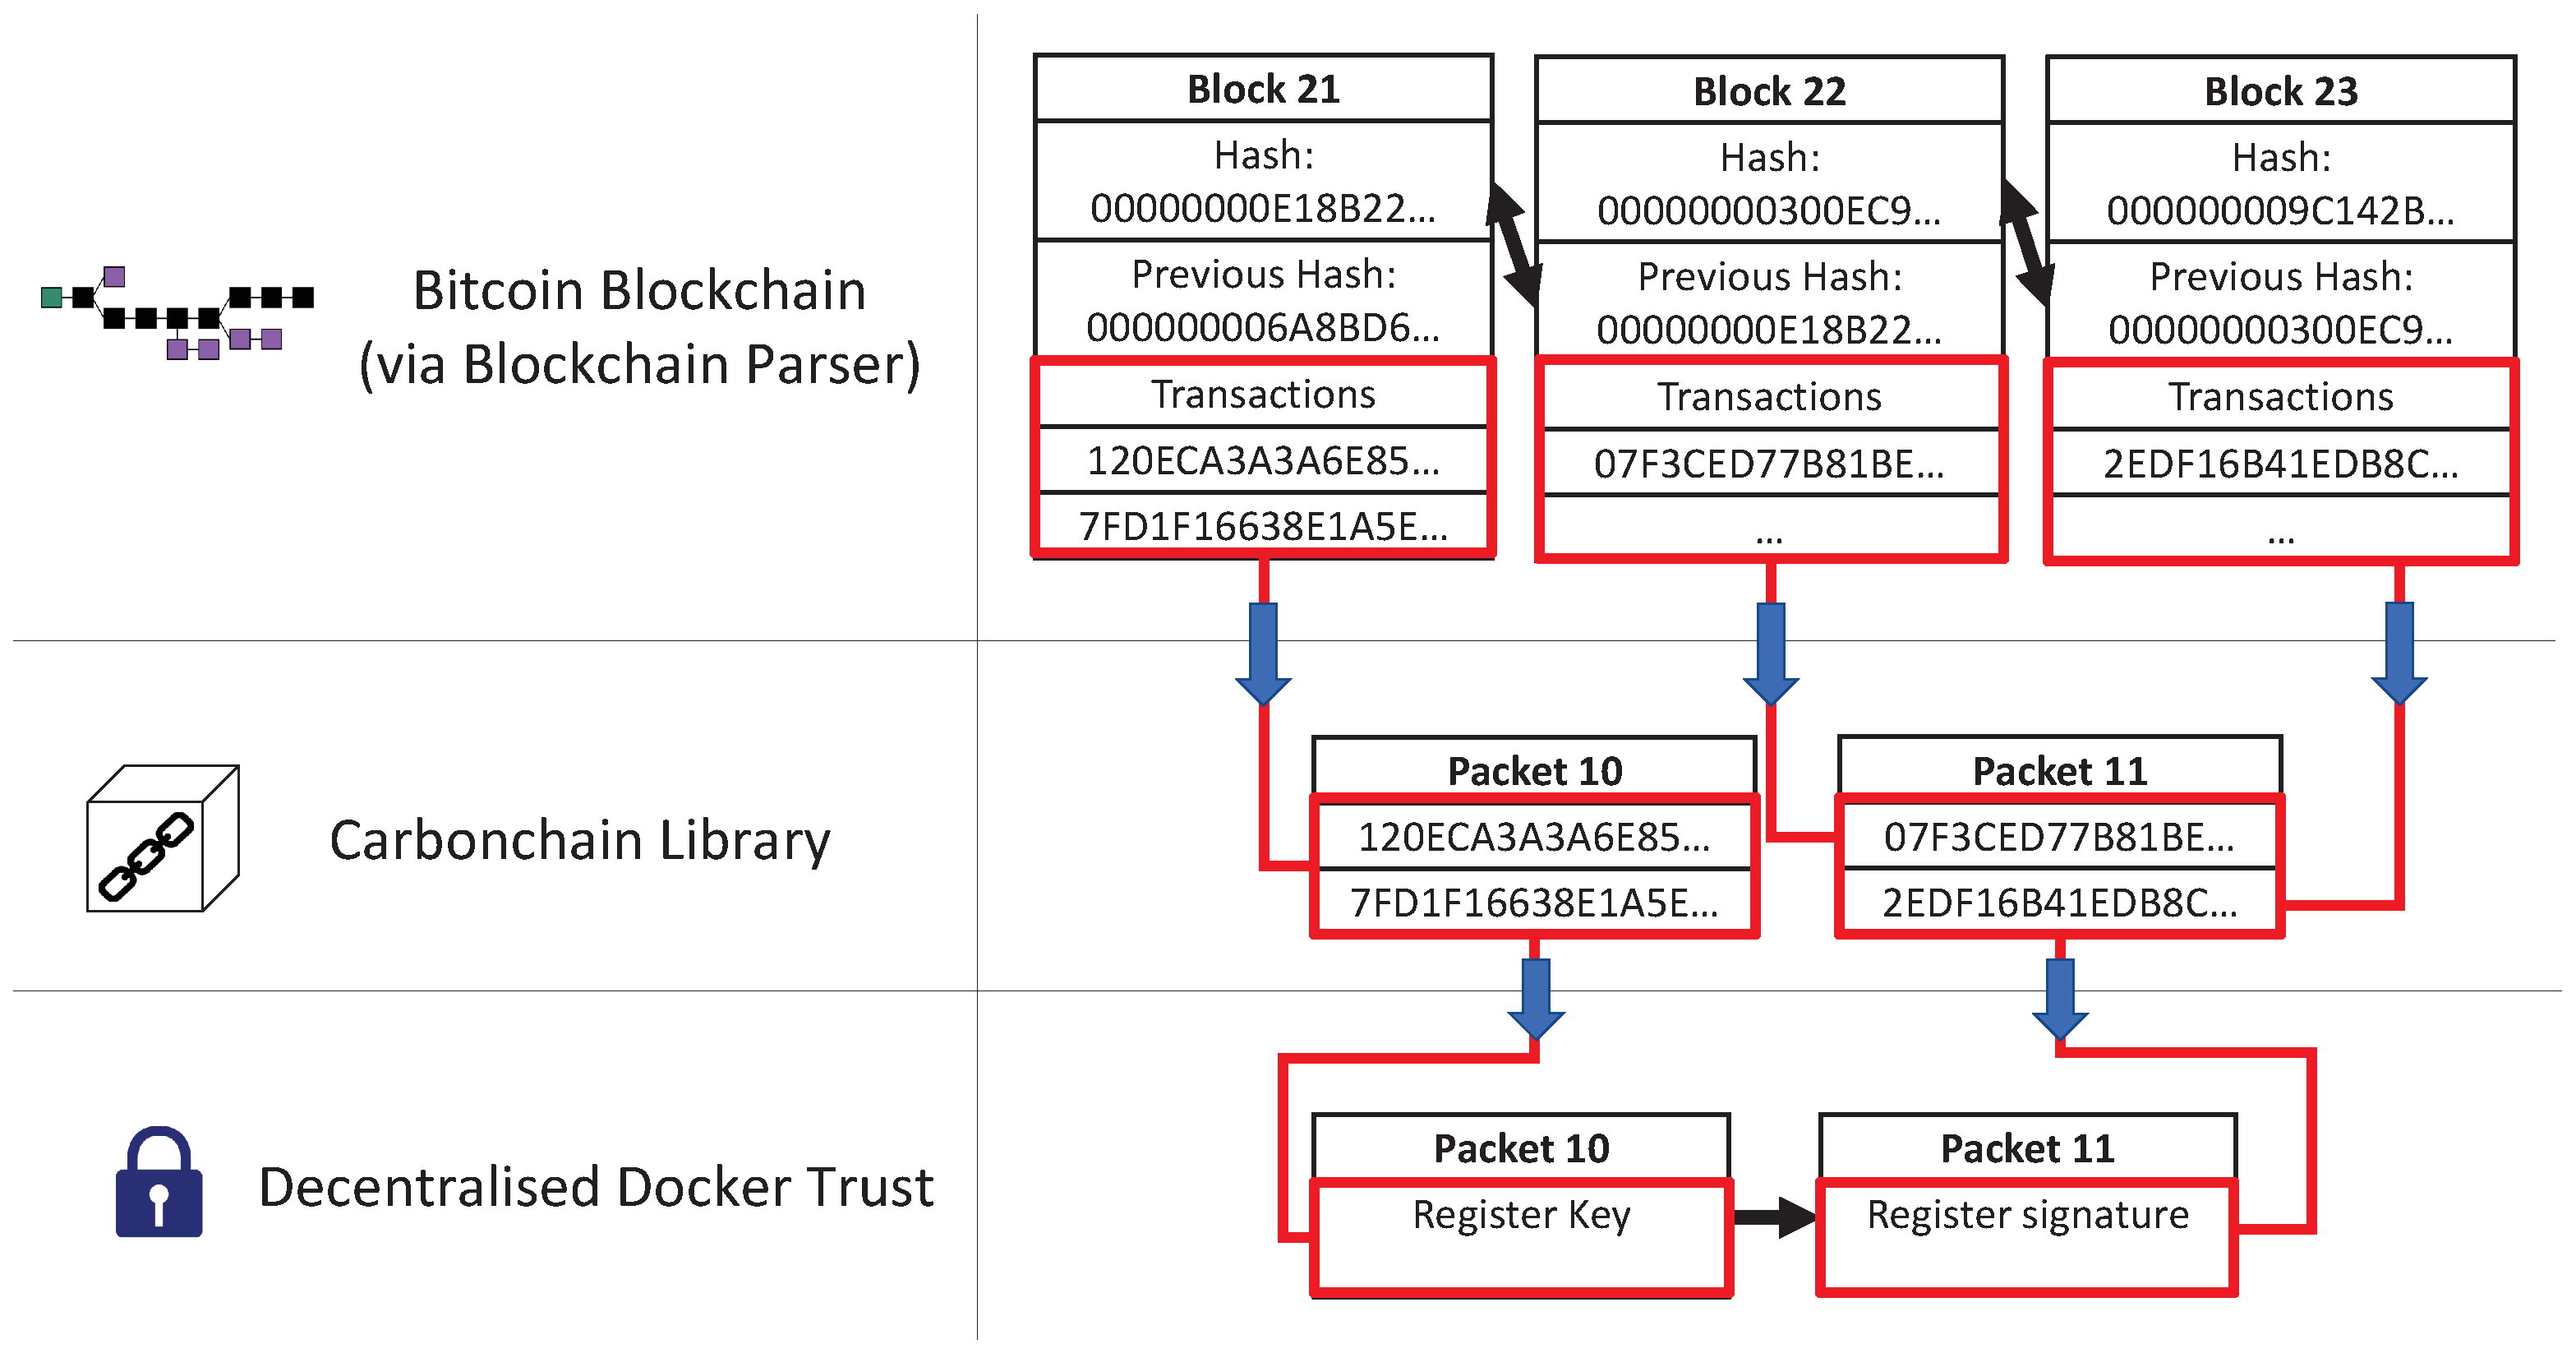
\includegraphics[width=1\linewidth]{DDTflow}
		\caption{Process of reading data}
		\label{fig:ddtflow}
	\end{figure}
	
	\noindent The full list of \ac{DDT} commands, \ac{REST} \ac{API} methods and payload breakdown for the different commands can be respectively found in Tables \ref{ddtcmd}, \ref{restapi}, \ref{regdelroot}, \ref{regdelsig} and \ref{regdelmeta} of Appendix D.}
	\subsection{Docker and IoT}
	{\par	
		\iffalse Docker is a lightweight application which allows for rapid deployment of containers. Using AUFS or overlayFS as its storage driver, it isolates read-writes of applications to within the container. This reduces I/O load and storage space needed as multiple versions of files will not be required [1,2]. Furthermore, IoT devices are generally lightweight and small, with storage space ranging from 4GB to 128GB [3]. Due to space constraints, installing full-sized applications on IoT devices is not feasible.

		IoT devices are built with a focus on light computing, which is a reason why processors for IoT devices run on low power and have low RAM. Using Docker, applications can run with minimal performance overhead [4] on its limited hardware. Taking a look at IoT devices such as the Raspberry Pi where add-ons can be added via the use of I/O extensions, the capability and functions of the device can be expanded. As Docker runs each application in its own container, all data, functions and software are isolated within its own container and do not interact with other containers and the host Operating System (OS) [5]. 
		\\\newline
		Attacks such as privilege escalation will be fully contained within the affected container and operations in other containers and the OS will continue as per normal. For example, an IoT device can contain temperature, humidity and a sunlight sensor. An attacker exploiting a bug in the temperature sensor should only affect the specific container in which the affected sensor is running on, as all containers are isolated from each other and the host OS, resulting in continued operations.\\\newline \fi
		
		\ac{IoT} is the infrastructure consisting of smart networked devices and other embedded devices that collect and exchange data. Such devices include sensors, household electronics, industrial device and etc. Through the use of \ac{IoT} devices, personal experience can be customised through the collection of data and to offer specific services to the user while preserving privacy and security.\\\newline
		Docker is a lightweight application which allows for rapid deployment of containers. Using its \textit{union filesystem} driver, it isolates read-writes of applications to within the container. This reduces \ac{I/O} load and storage space needed as multiple versions of files will not be required. Furthermore, it must be noted that many \ac{IoT} devices are not built with powerful hardware similar to those used in high-end smartphones, consumer desktops or even servers. It is therefore more likely that an application with a lighter footprint such as Docker will be preferred over the use of traditional \ac{VM}s.\\\newline
		Security of \ac{IoT} devices will also need to be considered as attackers will consider \ac{IoT} devices to be a potential attack vector. Common attacks such as the use of privilege escalation will be fully contained within the affected container while other containers and the \ac{OS} will continue to function normally. For example, an \ac{IoT} device may contain a temperature, humidity and a sunlight sensor. An attacker exploiting a bug in the temperature sensor will only affect the specific container in which the temperature sensor is running on, as all containers are isolated from each other and the host \ac{OS} \cite{consec}, resulting in continued operations.
		\noindent \iffalse References:\\\newline
		[1]: What is AUFS (Advanced Multi-Layered Unification Filesystem)? - Definition from WhatIs.com. (n.d.). Retrieved May 29, 2017, from http://searchaws.techtarget.com/definition/AUFS-Advanced-Multi-Layered-Unification-Filesystem
		\\\newline
		[2]: Use the OverlayFS storage driver. (2017, May 26). Retrieved May 29, 2017, from https://docs.docker.com/engine/userguide/storagedriver/overlayfs-driver/
		\\\newline
		[3]: RPi SD cards. (n.d.). Retrieved May 29, 2017, from http://elinux.org/RPi\_SD\_cards
		\\\newline
		[4]: Flux7, award-winning IT consultancy focused on cloud, containers, CI/CD and configuration managemen Follow. (2014, August 24). Performance of Docker vs VMs. Retrieved May 29, 2017, from https://www.slideshare.net/Flux7Labs/performance-of-docker-vs-vms
		\\\newline
		[5]: Your Software is Safer in Docker Containers. (2016, August 26). Retrieved May 29, 2017, from https://blog.docker.com/2016/08/software-security-docker-containers/
		\fi
	}

	\subsection{Ethereum}
	{\par \noindent Ethereum is a decentralised digital currency similar to Bitcoin but is specialised for use with smart contracts. Ethereum, similar to alternative cryptocurrencies, is based on blockchain technology and hence it has a 100\% uptime if there is at least one fully synced node that is online at any time. Ethereum provides more functionality than Bitcoin, allowing anyone to create decentralised applications and smart contracts with arbitrarily defined ownership rules, transaction formats and state transition functions.\\\newline
	Ethereum has advertised itself with the ability of allowing users to create their own cryptocurrency, personalising it with the users' customisations. It can also be used to issue assets such as organisational membership and even shares. Other applications that can be hosted on the Ethereum platform include a crowdfunding project or building an autonomous democratic voting system with full transparency and impartiality due to absence of human intervention and control. Ethereum has also been the blockchain of choice due to its low block creation time and smart contract features, as pointed out through the trial of Project Ubin by Monetary Authority of Singapore (MAS) \cite{ubinchain}. The full list of projects can be found on an independent party's link through the Ethereum website \cite{ethproj}. \\\newline
	Ethereum recommends the use of the language \textit{Solidity} for creation of its smart contracts. Solidity is a language designed around ECMAScript syntax so web developers will find it easier to learn and pick up, due to similarities with JavaScript.\\\newline
	It is important to note that the base unit of currency in Ethereum is measured in $wei$ and not $ether$. However, as the base unit of $wei$ is extremely small ($10^{-18}$ $ether$), $ether$ continues to remain the most commonly used term when dealing with currency in Ethereum. Table \ref{ethcur} details the different units of currency in Ethereum.
	\begin{table}[H]
		\centering

		\begin{tabular}{|l|l|}
			\hline
			\rowcolor[HTML]{C0C0C0} 
			Unit                & Wei Value   \\ \hline
			Wei                 & 1 wei       \\ \hline
			Kwei (babbage)      & $10^3$ wei  \\ \hline
			Mwei (lovelace)     & $10^6$ wei  \\ \hline
			Gwei (shannon)      & $10^9$ wei  \\ \hline
			microether (szabo)  & $10^{12}$ wei \\ \hline
			milliether (finney) & $10^{15}$ wei \\ \hline
			ether               & $10^{18}$ wei \\ \hline
		\end{tabular}
			\caption[Ethereum currency denominations]{Ethereum currency denominations \cite{ethcur}}
	\label{ethcur}
	\end{table}
\noindent Each user of Ethereum has a wallet (or keystore) to store ether. The generation of this wallet involves the creation of a private key and a public key. The private key is generated using \ac{ECDSA}, specifically the secp256k1 curve. The public key is then generated using the details from the private key. The last 20 bytes of the public key will determine the wallet address of the user.\\\newline
Other notable cryptographic libraries used in Ethereum are Scrypt for \ac{KDF}, \textsc{Keccak} hash algorithm for \ac{HMAC} and AES-128-CTR (Advanced Encryption Standard, 128-bits with Counter Mode) for cipher. CTR is used due to advantages in using parallelisation (i.e. quicker encryption/decryption).
	\iffalse 
	cryptocurrency that was based on the blockchain structure. Developers of Ethereum referenced the structure of Bitcoin and adapted/improved the cryptocurrency. Technically a smart contract system using blockchain. Scripting of contracts is mainly scripted in a language called Solidity (Heavily based on ECMAScript as web developers would find syntax familiar).\fi}
\subsubsection{Essential Terminologies}
{\par Ethereum introduces new terminologies that are unique to its platform and fundamental in understanding later sections in this paper.}
\begin{enumerate}
	\item Gas: Gas is a measurement of computational steps required for an action in the transaction to be successful. Each unit of Gas cost $wei$. Ethereum allows users to specify the price for each unit of gas ($\geq0$). Users can set the price for gas depending on how fast the transaction needs to be propagated into the blockchain. There are also safeguards in place with the use of Gas, such as being required to specify a ``Gas Limit''. This allows the user to state the maximum amount of Gas the user is willing to spend for the transaction and to ensure that the user never runs of funds (especially in the case of infinite loops). If the computation involved exceeds the ``Gas Limit'', then computation is stopped and any computation completed up to that point is still paid to the miner.
	\item Uncles: Uncles are essentially stale blocks that are not on the longest chain in the blockchain. This usually happens when there is a network issue and the first miner is unable to announce the formation of a new block in the blockchain and as a result, another miner has overtaken the first in adding his block into the blockchain. In Ethereum, miners who find Uncles are still rewarded for their effort (albeit smaller) and their contribution in strengthening the security of the blockchain.
\end{enumerate}
\subsubsection{Block Architecture}
{\par Ethereum's block data contains 3 Merkle-Patricia trees while the header consists of 15 components. The 3 Merkle-Patricia trees in simplicity, are radix trees with extra complexity in data to reduce lookups. These 3 Merkle-Patricia trees are used to store data on the state of Ethereum accounts (State Root), list of all transactions of the block (Transaction Root) and receipts from each transaction of the block (Receipt Root). All hashes in Ethereum use the \textsc{Keccak} algorithm unless stated otherwise. The headers and explanation for each of the header fields are as follows:
	\begin{enumerate}
		\item Previous Hash: A 256-bit hash of the previous block's block header.
		\item Nonce: A 64-bit hash such that when combined with ``Mix Hash'', proves that sufficient amount of computation has been done to generate the hash of the block that satisfies the proof of work.
		\item Timestamp: The time in UTC that the block was created.
		\item Uncles Hash: A 256-bit hash of the list of uncles on blockchain height $n-1$.
		\item Beneficiary: 160-bit Ethereum address of miner where the fees from the mining will go to.
		\item Logs Bloom: Indexed information of all transactions in the block.
		\item Difficulty: Level of difficulty in mining the block
		\item Extra Data: Byte array containing data relevant to the block ($\leq$ 32 bytes).
		\item Number: Block number of block in the blockchain.
		\item Gas Limit:  Limit of gas that is allowed to be used per block.
		\item Gas Used: Amount of gas used for transaction in current block.
		\item Mix Hash: A 256-bit hash such that when combined with ``Nonce'' which proves that sufficient amount of computation has been done to generate the hash of the block that satisfies proof of work.		
		\item State Root: A 256-bit hash of the root node of the radix tree after all transactions are executed and finalisations applied (Information of all accounts in the blockchain).
		\item Transactions Root: A 256-bit hash of the root node of the radix tree after it has been populated with all transactions of the block.
		\item Receipts Root: A 256-bit hash of the root node of the radix tree after it has been populated with receipts for each transaction in the block.
	\end{enumerate} 
Figure \ref{fig:ethblkstruct} provides a graphical representation of Ethereum's block architecture.}
\begin{figure}[H]
	\centering
	\includegraphics[width=1\linewidth]{ethereumblkstruct}
	\caption[Ethereum Block Architecture]{Ethereum Block Architecture \cite{ethblkarc}}
	\label{fig:ethblkstruct}
\end{figure}
\noindent In the case of Ethereum, if the state of accounts are not changed, the respective nodes of the trie will refer to the trie of the block in which the state was changed. This method of referencing reduces the size of the block by preventing excessive duplication of data across multiple blocks.
	\subsection{Light Wallet}
	{\par \noindent
		Performing transactions for cryptocurrencies on embedded devices or other devices such as mobile phones and tablets is not feasible given the growing size of the blockchain and the computation required to verify all the blocks. Even on computers, the growing size of the blockchain may pose a problem for users who have limited storage space. Due to limitations in hardware capabilities of these devices, an alternative method is needed for verification and syncing of blockchain data. \ac{SPV} (also known as \ac{LES} for Ethereum) is a technology where only block headers and relevant block data are downloaded to reduce the total memory and space footprint on the device. If required, an additional step of storing key-value pairs in a \ac{DHT} is performed.\\\newline
	The process is simple:
\begin{enumerate}
	\item The \ac{SPV} client contacts full nodes (that has data of the entire blockchain) and downloads all block headers from the nodes.
	\item Using bloom filters, the client filters the relevant information from the Logs Bloom located in the block header.
	\item It will search the transaction receipts trie matching of the matching block headers.
	\item \ac{RLP} of the transaction is checked to see if the data matches.
	\item The client will then output the query result.
\end{enumerate}}
	\subsection{Cryptocurrency Mining}
	\label{mining}
	\textit{Mining} is the process of adding transactions to the block. Before the block can be accepted by other network participants and propogated into the blockchain, the system (miners) must prove that it has completed a significant amount of work by requiring that the calculated hash of the block satisfies the condition of having $x$ number of leading zeros. For example, in figure \ref{noncepow}, we require a hash to be a string beginning with 3 leading zeroes (`000'). We perform this computation by adding nonces (integers incrementing from 0) to the end of the data string and in this case the nonce that satisfies the condition is 4250. The number of leading zeroes required is determined by the \textit{difficulty}, which is dynamically adjusted to ensure that new blocks are generated once every 10 minutes (for Bitcoin) or 15 seconds (for Ethereum). This entire computational process is known as the \textit{Proof of Work}. 
	\begin{figure}[H]
		\centering
		\includegraphics[width=1\linewidth]{noncepow}
		\caption{Nonce and \textit{Proof of Work}}
		\label{noncepow}
	\end{figure}
	\noindent Calculating a hash requires many rounds of trial and error, which is computationally intensive and time-consuming as compared to verifying the hash.
\subsubsection{Hardware Capabilities}
\subsubsubsection{Bitcoin Mining}
{\par \noindent
In the current section, the discussion on hardware performance is based on data obtained from the Bitcoin network as it is relatively more mature than other cryptocurrencies and has a page detailing the hash rates of different hardware \cite{nonspechw,spechw}. \\\newline
The inception of Bitcoin in 2009 required the use of a \ac{CPU} for cryptocurrency mining as specialised hardware was absent. Analysis of the data shows that for the \ac{CPU}s released to date, the maximum hash rate was 140 Mhash/s for Intel's Xeon Phi 5100 and 115 Mhash/s for \ac{AMD}'s 4$\times$ Opteron 6174. It must be noted that the two processors mentioned are for server architectures and the cost is not easily justifiable for consumer use. Results from \ac{ARM} are not considered as the best performing processor, the Cortex-A9 can only reach a maximum of 1.3 Mhash/s and the result is significantly smaller than any Intel or AMD \ac{CPU} for any meaningful conclusion to be drawn. Considering that the current hash rate of the network is approximately $5\times10^{15}$ hash/s \cite{bchashrate}, it would require an estimated $3.\overline{571428}\times10^7$ of \ac{AMD}'s server processors.
\\\newline
The \ac{GPU} progressively took over \ac{CPU}'s role in mining. \ac{CPU} mining continues to exist today, despite being unprofitable. \ac{GPU}s are able to outperform \ac{CPU}s in magnitudes of hundreds or thousands, as each core in a \ac{CPU} is able to execute 4 32-bit instructions per clock on a 128-bit \ac{SSE} instruction or 8 instructions on 256-bit \ac{AVX}. For \ac{GPU}s, the number of instructions are dictated by the number of CUDA cores (NVIDIA) or ALUs (\ac{AMD}), usually in the thousands. Using NVIDIA's GTX590 as a benchmark, the hash rate recorded was $1.93\times10^8$ hash/s while 6$\times$ 5870 \ac{GPU}s from \ac{AMD} had a hash rate of $2.568\times10^9$ hash/s. This makes \ac{GPU}s more attractive than \ac{CPU}s as the performance/cost ratio is many times higher. Also, the difficulty of the block will increase in proportion to the increased hash rate, hence \ac{CPU}s are deemed too slow for any mining activity.}
\\\newline
\ac{FPGA} was subsequently introduced. \ac{FPGA} chips are programmable by the user, so specialised software was written for these chips to calculate the hashes (Bitcoin's \textsc{SHA-256}) faster and more efficiently than \ac{CPU}s or \ac{GPU}s. As the chips were programmable, it was convenient for users who were holding it to re-purpose the chips from their original functions to a Bitcoin miner. Due to \ac{FPGA}'s small chip size, low power usage and high hash rates (Highest being $2.52\times10^{10}$ hash/s), \ac{FPGA} miners were able to obtain much more rewards from mining while the difficulty of mining continued to increase exponentially.\\\newline
The current generation of Bitcoin miners employ \ac{ASIC} for mining. These chips were specially designed and manufactured for the sole purpose of calculating the Bitcoin hashes. Like \ac{FPGA}, these chips were small and could come in form factors like a USB stick. An important difference between \ac{ASIC} and \ac{FPGA} is that \ac{ASIC} is not user programmable after manufacture and has only one purpose. These chips contain massive computing power and data centres with racks of \ac{ASIC} have subsequently been commissioned. When taking a look at the list of \ac{ASIC} chips, we find that many have been deprecated as the hash rates are unable to keep up with the trend. However, AntMiner continues to dominate in the field of hashing power. Their latest product, the AntMiner S9 has an advertised hash rate of $1.4\times10^{13}$ hash/s. This \ac{ASIC} chip has the power equivalent to 550 times the fastest \ac{FPGA} chip. \\\newline
From the analysis above, it is reasonable to conclude in general that Bitcoin mining is computationally heavy and requires a lot of specialised hardware for a small fraction of the network hash rate. New users going into mining without doing prior research may not be able to recover their initial investments. 
	\subsubsubsection{Ethereum Mining}
	Ethereum is similar to Bitcoin, in that it requires computation of hashes. However, Ethereum employs the algorithm \textsc{Ethash} (Based on Dagger-Hashimoto) instead of \textsc{SHA-256}. \textsc{Ethash} is unique in that it is a  \textit{memory-hard} algorithm. The primary reason for using a memory-hard algorithm is to ensure that using specialised hardware will not have an advantage due to large memory requirements, allowing casual users to now participate in propagating the blockchain with common hardware.\\\newline
	Understanding the Dagger Hashimoto algorithm establishes the premise for further analysis on the feasibility of employing different hardware for the sole purpose of mining. \\\newline
	The Dagger Hashimoto algorithm combines the need for memory reads and the storage of \ac{DAG} in memory. A \ac{DAG} is a finite directed graph with topological ordering such that any edge will connect a vertex of a smaller order to a vertex of a larger order in the sequence, with no cycles being formed. This \ac{DAG} is regenerated every 30000 blocks (approximately 100 hours) and the current size of the \ac{DAG} has exceeded 2GB. 
	\begin{figure}[H]
		\centering
		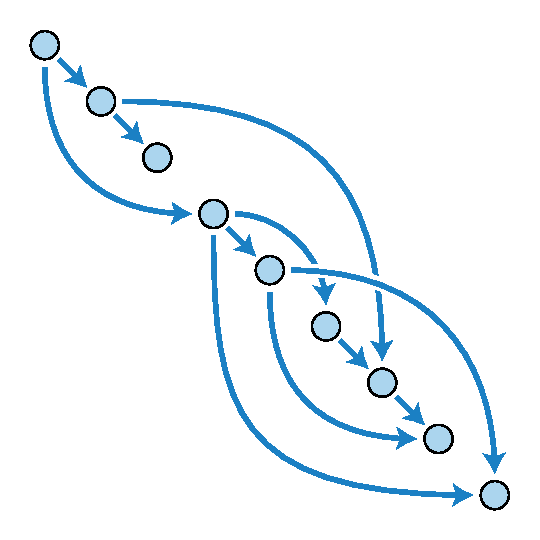
\includegraphics[width=0.3\linewidth]{dag.eps}
		\caption[Directed Acyclic Graph]{Directed Acyclic Graph \cite{DAG}}
		\label{fig:dag}
	\end{figure}
	\noindent For \ac{ASIC} miners to be profitable on the Ethereum platform, each processor must have sufficient memory available to store the \ac{DAG}, have room for the growing size of the \ac{DAG} and have fast read speeds to read the \ac{DAG} from memory when computing hashes. This combination of algorithms currently makes it impossible to implement high capacity memory on \ac{ASIC} chips and as a result the algorithm used by Ethereum is \ac{ASIC} resistant and hence useless. \ac{GPU}s with less than 2GB of memory have also been affected by the growing size of the \ac{DAG} and are unable to mine Ethereum blocks.\\\newline
	Therefore, participants on newer and more recent \ac{GPU}s will find themselves being able to make profits while contributing to the strengthening of the blockchain.
	\subsubsection{Pool Mining}
	\label{poolmine}
	Miners with significantly lower hash rates may find themselves being unable to mine whole blocks fast enough to compete with the network. The success rate of mining a block can be attributed to the following formula:
	\begin{equation}\label{eq:1} p_{solo}=\frac{\textit{$HRate_{User}$}}{\textit{$HRate_{Network}$}}\end{equation} where $HRate$ represents the hash rate. We calculate the total hashrate of each user based on all running cryptomining hardware the user owns. Analysing further, the hash rates of the user and the network are directly proportional to the number of blocks that the user will mine successfully and the number of blocks generated, i.e. the user will successfully mine 1 block out of every $\frac{1}{p}$ blocks and obtain the respective block reward.\\\newline
	Additionally, 144 blocks are generated each day for Bitcoin (one every 10 minutes) or 5760 blocks per day for Ethereum (one every 15 seconds). Hence the number of days required to mine one block successfully can be calculated per this formula:
	\begin{equation}\label{eq:2}
	D(p)=\begin{cases}\frac{1}{144p_{solo}}&\text{if Bitcoin}\\\frac{1}{5760p_{solo}}&\text{if Ethereum}\end{cases}
	\end{equation}
	From formulas (\ref{eq:1},\ref{eq:2}), two conclusions can be formulated,
	\begin{enumerate}
		\item When $HRate_{User}$ is low, the success rate of mining a block $p$ is decreased.
		\item When $p_{solo}$ tends close to $0$, $D(p)$ will increase and is an indicator that a low hash rate will eventually lead to a higher time in obtaining returns. This is the reason \ac{CPU} mining is not recommended.
	\end{enumerate}
It has not been mentioned specifically in this section, but the difficulty also affects the days required to mine one block. In general, the network hash rate follows an increasing exponential graph \cite{bchashrate}. This inevitably leads to a continued decrease of $p$ and the number of days required will be more than the theoretical $D(p)$ that has been calculated.\\\newline
In summary, miners who do not have adequate hardware will be unable to mine blocks and receive returns from investments made on hardware. To alleviate this problem, miners could join mining pools. This makes it convenient to both miners and mining pools for multiple reasons,
\begin{enumerate}
	\item Mining pools will be able to obtain more blocks based on the total hash rate of all users who connect their miners to the pool.
	\item Due to the reason above, owners of mining pools can charge a small fee for providing the pool service to miners. 
	\item Users with lower hash rates will obtain the block reward based on the percentage of computing power contributed to mine the block. (As opposed to solo mining where there is no guarantee that a miner would be able to successfully mine a block)
\end{enumerate}
 This is advantageous for casual users as block rewards can now be easily obtained, however small the contribution.\\\newline
 Adapting formula (\ref{eq:1}) for mining pools yields the following formula,
 \begin{equation}\label{eq:3}
 p_{user}=\frac{HRate_{User}}{HRate_{Pool}}\times\frac{HRate_{Pool}}{HRate_{Network}}
 \end{equation}
 The formula for number of days to now obtain the same number of cryptocurrency from mining can be adapted from formula (\ref{eq:2}),
 	\begin{equation}\label{eq:4}
 D(p)=\begin{cases}\frac{1}{144p_{pool}}&\text{if Bitcoin}\\\frac{1}{5760p_{pool}}&\text{if Ethereum}\end{cases}
 \end{equation}
 The formulas (\ref{eq:1},\ref{eq:3}) and (\ref{eq:2},\ref{eq:4}) may look exactly the same, however it is worth noting that pool mining (formulas (\ref{eq:3},\ref{eq:4})) allows payout of block rewards in percentage contribution to the block that was mined by the pool. The formulas (\ref{eq:1},\ref{eq:2}) for solo mining only assumes two event outcomes, either the block is successfully mined or it is not. It is therefore more reasonable to conclude that mining in a pool would yield a stable flow of reward to the miner as compared to mining solo for those with a lower hash rate.
 \subsubsection{Mining Protocols}
 {Before the current Stratum protocol was introduced for mining cryptocurrencies, various protocols that were previously used but were not favoured due to bottlenecks and/or scalability issues which will be explained in-depth in the following sections.}
 \subsubsubsection{Original Protocol}
 {\par The original protocol started with Bitcoin, did not give control to the miner over the various aspects of block creation, such as the selection of transactions for addition into the blocks. The server will instead issue the headers with all the details included and only required the miners to compute the nonce through iterative hashing. Once a valid nonce has been found, the result would be sent back to the server and the block would be propagated into the blockchain. New work would subsequently be requested if mining continued. This was when \ac{CPU} mining was the norm.\\\newline
 	It is clear that the recorded exponential increase in the Bitcoin network's hash rate \cite{bchashrate} will create severe bottlenecks in the network bandwidth between clients and the server.
 	\subsubsubsection{Getwork}
 	{\par \noindent Getwork was subsequently created, the changes primarily in data transfer. The Getwork protocol involves the use of JSON-\ac{RPC} method over HTTP transport. The use of HTTP reduces the effort required in establishing a new data transport system as existing infrastructure can be utilised for movement of data.\\\newline
 	The process involves multiple steps and encoding conversions \cite{getwork}, which has been detailed below.
 \begin{enumerate}
 	\item Data is sent to the miner in \textbf{little-endian} encoding
 	\item The miner re-encodes the data to \textbf{big-endian} through swapping the order of each pair of hexadecimals in a set of 32 bits (with the Least Significant Byte first to Most Significant Byte last). This conversion is required as the encoding of \textsc{SHA-256} is in big-endian.
 	\item The last 64 bits of the hexadecimal data is read and converted into a value.
 	\item The value calculated in the previous step indicates the size of data that is preserved (counting from the front). Any additional data that exceeds this size is subsequently deleted.
 	\item The resulting data is put through the \textsc{SHA-256} algorithm hashed twice (double hashing).
 	\item The miner re-encodes the obtained hash back to \textbf{little-endian} before transmitting the data back to the server.
\end{enumerate}}
 	\subsubsubsection{Getwork + rollntime Extension}
{\par \noindent An extension to the Getwork protocol was subsequently made to address the issue of not being able to provide a valid nonce for a given header. The rollntime extension, as it is called allows a miner to update the timestamp with a tolerance of $t$ seconds. Doing so will cause the hashes to change and in turn reduce the probability of a valid nonce not being found within an entire nonce range ($2^{32}-1$).\\\newline This framework suffers the same bottlenecks as the original protocol when the hash rate is scaled up exponentially. If we were to consider a miner with the capability of mining at a rate of $4.3*10^{10}$ hash/s, then this would be the equivalent of exhausting 10 nonce ranges per second ($10\times(2^{32}-1)$). Putting it into perspective, the miner would need to request for 10 block headers every second. Doing so over HTTP transport system causes tremendous stress over the HTTP network.}
\subsubsubsection{GetBlockTemplate}
{\par \noindent Getwork was soon deprecated in favour of \ac{GBT}. \ac{GBT} moves the block creation control from the server to the miner, including any transactions to be added into the blockchain. With this system, miners now have full control over the mining process. As a result of this modification, the size between blocks will differ, depending on the amount of transactions being included into each block. This would translate to miners requesting for more transactional details. \ac{GBT}, like its predecessor Getwork, uses the HTTP transport for data transfer and the same persistent issues on network bottlenecking continue to plague these protocols. It is however notable that some mining pools continue to support this protocol, but many others have moved to the newer Stratum protocol.}
\subsubsubsection{Stratum}
{\par \noindent Stratum was originally created for the lightweight client Electrum and was later adopted to replace the Getwork protocol in 2012. Stratum was designed as a text-based protocol, with the primary reason being it could be easily read by humans and systems \cite{stratumprot}. Developers would be able to add extensions to future versions of the protocol while being able to maintain backwards compatibility. Stratum encodes its payload as JSON-\ac{RPC} messages and uses a \ac{TCP} socket to transmit messages. Since Stratum does not depend on HTTP transport, there is minimal network overhead on the systems.\\\newline
Furthermore, integrating Stratum with systems was simpler as miners would already have JSON libraries implemented on their systems (due to use in other mining protocols at that time). Not relying on HTTP also meant that redundant data such as mining extension flags and HTTP headers itself could be removed, trimming space and reducing bandwidth cost on the network in overall. The result is a system that could easily broadcast messages in a timely manner without slowdowns and bottlenecks in the network. To the miner, using this protocol allows faster switching in the event the block that is to be mined changes and reduces the number of stale blocks generated by miners over the network (as well as the rejected share ratio). \\\newline By default, modern cryptocurrencies that employ Proof-of-Work mining now support Stratum.}
		\subsection{Rewards}
		\label{reward}
		\subsubsection{Bitcoin}
As an incentive to get miners to secure the blockchain, each block that is mined gives the miner a block reward, as well as any transaction fees from transactions that were added to the respective block. For Bitcoin, block rewards start at 50 BTC (Bitcoins) per block and are halved every 210000 blocks. The current block reward is 12.5 BTC.\\\newline
We consider $n$ as the block number (starting from 0) and take $n$ to be significantly large. Then the maximum amount of Bitcoins that can be circulated is
\begin{equation}\label{eq:5}
210000\sum_{i=0}^{\infty}\frac{50}{2^i} = 21000000
\end{equation}
and the upper bound on the number of BTC currently circulating at any time can be deduced using the following formulas.
\begin{flalign*}
m=n+1&\quad \text{(Define m to be the block number starting from 1)}\\
j=\floor*{\frac{m}{210000}}&\quad \text{(Define }j\text{ to be the batch number of 210000 blocks{)}}
\end{flalign*}
\begin{equation}\label{eq:6}
BTC_{Total}=
\begin{cases}
m\times 50& m\leq210000,\\
210000\displaystyle\sum_{i=0}^{j-1}\frac{50}{2^i}+m\bmod210000\times\frac{50}{2^{j}}&\text{otherwise}
\end{cases}
\end{equation}
In theory, equation (\ref{eq:6}) will allow us to determine the amount of BTC there is in circulation for any given time. However, this formula does not take into account cases where loss of wallets and purposeful destruction of currency have occurred. This issue becomes more apparent as Bitcoin becomes more mature. It is therefore reasonable to conclude that the amount of usable BTC is less than the $BTC_{Total}$ calculated in equation (\ref{eq:6}).
\subsubsection{Ethereum}
For Ethereum, each block mined gives miners a static value of 5 ether. Uncles that are included in a block receive an award of $\frac{1}{32}$ of the static block reward, or 0.15625 ether. Miners that created uncle blocks will also obtain a reward of $\frac{7}{8}$ of the static block reward, or 4.375 ether. Bitcoin on the other hand does not reward miners for mining uncles (or stale blocks). Ethereum has no upper limit on the total amount of ether that is being circulated. It has however been predicted that the rate of loss of wallets and purposeful destruction of currency will balance with the ether that is being created, which would result in a stabilisation of the amount of usable ether in the system.
\subsection{Value of Cryptocurrency}
{\par As previously stated in sections \ref{mining} and \ref{reward}, we can conclude that the rewards obtained from mining can be summarised into the following
	\begin{equation*}
	Rewards \propto \frac{Hash\text{ }Rate}{Difficulty}
	\end{equation*}
	Currently, more than half of the 21 million BTC (equation (\ref{eq:5})) is in circulation. The increase in the amount of BTC in circulation is expected to slow down to the halving of block rewards every 210000 blocks. Due to the cap on the number of BTC that can be created and the loss of BTC for reasons previously specified, it is understood that the intrinsic value of each unit of BTC will increase as the amount of BTC in circulation gradually decreases provided that the use of Bitcoin continues to be in widespread use as it is currently. In other words, Bitcoin will continue to experience continual deflation with time.}\\
{\par \noindent For Ethereum, there is no upper limit on the amount of ether in circulation. However, it is expected that the gain in ether due to mining and the loss due to accidental or purposefully destruction of ether will balance out. In other words, there will be no net gain or loss of ether in due time. As such, inflation/deflation beyond this point $t$ is expected to stabilise and the value of ether would depend on the demand of the cryptocurrency.}
	\subsection[Greedy Heaviest-Observed Sub-Tree]{Greedy Heaviest-Observed Sub-Tree (GHOST)}
	\ac{GHOST} was originally proposed in 2013 by academics Yonatan Sompolinsky and Aviv Zohar \cite{bitcoinghost}. The implementation recommended changing the definition of Bitcoin's main chain from the ``longest chain'' to ``heaviest chain''.\\\newline
	Currently, miners that face network propagation issues will continue to mine on their current chain they are able to synchronise their blockchain with the network. Eventually, this chain will be considered stale as other miners which have better networks will be able to broadcast their blocks earlier (therefore the system will recognise these blocks as valid). Scaling this problem up from solo miners to mining pools raises 2 prominent problems:
	\begin{enumerate}
		\item Waste of hashing power since blocks generated with proper headers and data may be considered stale by the network; and
		\item Frequency of stale blocks being generated increases in proportion to the increased amount of hashing power.
	\end{enumerate}
If we further consider the proposition of reducing block creation time, the probability of branching in the chain will significantly increase. Figure \ref{fig:ghost} provides a clearer illustration to this problem.\\\newline
\begin{minipage}{.45\textwidth}
\begin{figure}[H]
	\centering
	\includegraphics[width=1\linewidth]{ghost}
	\caption{Chain branching}
	\label{fig:ghost}
\end{figure}
\end{minipage}
\hfill
\vline
\hfill
\begin{minipage}{.52\textwidth}
	In this figure, we assume mining pool 2 to have network propagation issues. Hence, miners in mining pool 2 will continue to mine on the block that was recently found and extend their end of the chain. Once the mining pool has synchronised with the network, all blocks created by mining pool 2 that lie on the fork will be deemed as invalid as it does not satisfy the ``longest chain'' property.
\end{minipage}\\\vspace{1em}\newline
Consider the problem that the chain now has multiple forks. Suppose there was an attacker plotting a ``double-spend'' attack, then the attacker would require significantly less than 50\% of the network hash rate, depending on the degree of forking on the chain.
\begin{figure}[H]
	\centering
	\includegraphics[width=0.7\linewidth]{ghost2spend}
	\caption{Double-spend attack with ``longest chain'' principle}
	\label{fig:ghost2spend}
\end{figure}
\noindent By implementing \ac{GHOST}, we select the valid chain based on its \textit{weight} rather than its length. We calculate the weight of the chain by taking the block before the fork as the root node of the subtree, and count the number of nodes (blocks) that are in every branch. We select the branch that has the largest number of blocks and repeat for every level until the heaviest chain has been determined. In terms of the algorithm, we can implement the following psuedocode:
\begin{algorithm}
	\caption{Determine Heaviest Chain}\label{heavychain}
	\begin{algorithmic}[1]
		\State{Select \textit{root node} as block before branching}
		\For {$\text{subtree }level \leq \text{subtree }height$}
			\State {Calculate number of nodes (blocks) below the subtree level}
				\If {subtree has highest number of nodes}
				\State{Mark all nodes in the lower levels as valid}
				\Else
				\State{Mark all nodes in the lower levels as stale}
				\EndIf
			\EndFor
	\end{algorithmic}
\end{algorithm}\\
Revisiting the double-spend attack while using the \ac{GHOST} protocol implementation, the attacker must now match the hash rate of the heaviest chain, which could be significantly more than the previous ``longest chain'' method. This makes it even more costly to obtain hardware for an attack on the blockchain network (Figure \ref{fig:ghost2spendheavy}).
\begin{figure}[H]
	\centering
	\includegraphics[width=0.7\linewidth]{ghost2spendheavy}
	\caption{Double-spend attack with ``heaviest chain'' principle}
	\label{fig:ghost2spendheavy}
\end{figure}
\noindent Using \ac{GHOST}, block creation times can be reduced significantly since forks will now be useful in the determining of the valid chain. This move could also contribute to the supporting of a higher frequency of transactions on the network, which may further incentivise retailers to use blockchain technology to facilitate payments as confirmations can be done quicker and sooner.\\\newline
Although the protocol has been proposed since 2013, it has not been implemented for Bitcoin. However, Ethereum has implemented a modified version of \ac{GHOST}, which takes into account \textit{Uncles} and rewards miners for including the data into the main chain. It is important to note that Ethereum adopts the ``longest chain'' principle, but have tweaked the algorithm such that \textit{Uncles} are now relevant and contribute to the security of the blockchain. This makes it harder for the root node of the subtree to be excluded if an attack were to occur after the fork.
\subsection{Proof of Stake}
\noindent The Ethereum network has publicly mentioned in their roadmap that the ultimate goal would be to transit from a Proof of Work scheme to Proof of Stake (Serenity) \cite{posswitch}. The move is fueled in part due to the amount of electricity being consumed for hashing on the Bitcoin network, which has been estimated that electrical comsumption is equivalent to Ireland \cite{elecbill}. Another point that would be solved by the transition would be centralisation risks as the new algorithm would discourage the use of mining pools and this will in part decrease the probability of a 51\% attack occurring on the network.\\\newline
Using proof of stake, the implementation removes the need for specialised hardware (such as \ac{ASIC} or \ac{FPGA}) or the use of large amounts of electricity. However, this concept requires that users (validators) have a certain amount of ether to act as a security deposit before they are able to participate (draft documents indicate a minimum of 32 ether is required \cite{posdraft}). The implementation will not generate any new monies as there will be no mining involved. Instead, only transaction fees will be paid to validators. In addition, malicious actors who attempt to validate an incorrect chain or multiple chains will have their security deposits forfeited. Therefore, the adoption of this system will generally involves negative net issuance of monies (burning of currency).\\\newline
With the transition to proof of stake, it will be possible to create new blocks faster (with conservative estimates at one block every 4 seconds) due to removal of mining difficulties. This would accelerate the goal of Ethereum being able to support a higher transaction volume in the same given amount of time.\\\newline
Light clients will additionally be able to synchronise extremely fast as it would only need to verify the validator set against the header to ensure that the details match since the authenticity of the data in each block will have a guarantee that is backed by validators' deposits.
\\\newline
Consider the instance that an attack were to happen on the blockchain with the proof of stake model. As proof of stake requires that users have a stake in the cryptocurrency, a 51\% attack would mean that the attacker must have at least 51\% of the entire network's currency. With information on the current exchange rate to be USD 210/ether (at time of writing of this report) and the amount of ether in circulation currently estimated at about 20 million (4 million blocks $\times$ 5 ether/block), the attacker would require about USD $2.142\times10^9$ worth of ether. This attack would be too costly compared to if it was mounted on a proof of work blockchain instead as hacking a mining pool and obtaining the fraction of the network hash rate would be easier.

	\newpage
	\section{Conclusion}
	Through this internship, research into containerisation highlights the significant role software virtualisation using programs such as Docker can do to transform traditional data centres to those that can perform multiple roles and easily be scaled.\\\newline
	Blockchain technology has also shown potential not only in terms of transferring of currency or running contracts with full transparency in the case of Ethereum. Traditional functions such as banking can now harness blockchain technology to simplify current systems and automate this process. With the properties of immutability and transparency, data can be stored in blockchains with the assurance that it will be permanent and unchanged. Privacy concerns can also be fulfilled with all users being anonymous and identifiable only through a hashed wallet address.\\\newline
	Potential future research can build upon the use of blockchains and could include being used for defence to transmit information in the event of disruption of communications or possibly a modification in the protocols to allow high volume of transactions to be conducted without long propagation times.
	\newpage
	\begin{thebibliography}{9}

\bibitem{opreturn}Almel. (2014, July 17). Explanation of what an OP\_RETURN transaction looks like. Retrieved July 23, 2017, from \href{https://bitcoin.stackexchange.com/questions/29554/explanation-of-what-an-op-return-transaction-looks-like}{https://bitcoin.stackexchange.com/questions/29554/explanation-of-what-an-op-return-transaction-looks-like}
		
\bibitem{blockchaindup}Armstrong, S. (2016, November 14). Move over Bitcoin, the blockchain is only just getting started. Retrieved June 04, 2017, from \href{http://www.wired.co.uk/article/unlock-the-blockchain}{http://www.wired.co.uk/article/unlock-the-blockchain}

\bibitem{DAG}Eppstein, D. (2016, May 20).Topological Ordering. Retrieved June 09, 2017, from \href{https://commons.wikimedia.org/wiki/File:Topological_Ordering.svg}{https://commons.wikimedia.org/wiki/File:Topological\_Ordering.svg}

\bibitem{medrec}Azaria, A., Ekblaw, A., Vieira, T., \& Lippman, A. (2016). MedRec: Using Blockchain for Medical Data Access and Permission Management. \textit{2016 2nd International Conference on Open and Big Data (OBD)}. doi:10.1109/obd.2016.11

\bibitem{PkgMgmtSec}Baker, S., Cappos, J., Hartman, J.H., \& Samuel, J. (2008). Package Management Security.

\bibitem{getwork}Bitcoin Wiki. (2011, June 7). Getwork. Retrieved July 25, 2017, from \href{https://en.bitcoin.it/wiki/Getwork}{https://en.bitcoin.it/wiki/Getwork}

\bibitem{nonspechw}Bitcoin Wiki. (2014, September 24). Non-specialized hardware comparison. Retrieved June 08, 2017, from \href{https://en.bitcoin.it/wiki/Non-specialized_hardware_comparison}{https://en.bitcoin.it/wiki/Non-specialized\_hardware\_comparison}

\bibitem{spechw}Bitcoin Wiki. (2010, December 24). Mining hardware comparison. Retrieved June 08, 2017, from \href{https://en.bitcoin.it/wiki/Mining_hardware_comparison}{https://en.bitcoin.it/wiki/Mining\_hardware\_comparison}

\bibitem{bchashrate}Blockchain Luxembourg S.A. (2009, January 3). Hash Rate. Retrieved June 08, 2017, from \href{https://blockchain.info/charts/hash-rate}{https://blockchain.info/charts/hash-rate}

\bibitem{posdraft}Buterin, V. (2016, September 19). Mauve Paper (Version 3). Retrieved June 20, 2017, from \href{https://cdn.hackaday.io/files/10879465447136/Mauve\%20Paper\%20Vitalik.pdf}{https://cdn.hackaday.io/files/10879465447136/Mauve\%20Paper\%20Vitalik.pdf}
\bibitem{ProtectCommunityRepo}Cappos, J., Diaz, V., Kuppusamy, T.K., \& Torres-Arias, S. (2016). Diplomat: Using Delegations to Protect Community Repositories. \textit{NSDI}.

\bibitem{DockerSec}Docker, Inc. (2016). \textit{Introduction to Container Security}. United States: Docker, Inc.

\bibitem{consec}Docker, Inc. (2016, August 26). \textit{Your Software is Safer in Docker Containers}. Retrieved May 29, 2017, from \href{https://blog.docker.com/2016/08/software-security-docker-containers/}{https://blog.docker.com/2016/08/software-security-docker-containers/}

\bibitem{ethproj}Ethercasts. (2015, April). STATE OF THE DAPPS. Retrieved June 07, 2017, from \href{https://dapps.ethercasts.com/}{https://dapps.ethercasts.com/}

\bibitem{ethcur}Ethereum Community. (2016). Ether. Retrieved June 07, 2017, from \href{http://www.ethdocs.org/en/latest/ether.html}{http://www.ethdocs.org/en/latest/ether.html}

\bibitem{decentralised}Goyal, S. (2015, July 01). Centralized vs Decentralized vs Distributed – Saurabh Goyal – Medium. Retrieved June 04, 2017, from \href{https://medium.com/@bbc4468/centralized-vs-decentralized-vs-distributed-41d92d463868}{https://medium.com/@bbc4468/centralized-vs-decentralized-vs-distributed-41d92d463868}

\bibitem{posswitch}Gupta, V. (2016, February 22). The Ethereum Launch Process. Retrieved June 27, 2017, from \href{https://blog.ethereum.org/2015/03/03/ethereum-launch-process/}{https://blog.ethereum.org/2015/03/03/ethereum-launch-process/}

\bibitem{51}Matonis, J. (2014, December 04). The Bitcoin Mining Arms Race: GHash.io and the 51\% Issue. Retrieved June 05, 2017, from \href{http://www.coindesk.com/bitcoin-mining-detente-ghash-io-51-issue/}{http://www.coindesk.com/bitcoin-mining-detente-ghash-io-51-issue/}

\bibitem{ubinchain}Monetary Authority of Singapore. (2017). Project Ubin: Central Bank Digital Money using Distributed Ledger Technology. Retrieved June 28, 2017, from \href{http://www.mas.gov.sg/Singapore-Financial-Centre/Smart-Financial-Centre/Project-Ubin.aspx}{http://www.mas.gov.sg/Singapore-Financial-Centre/Smart-Financial-Centre/Project-Ubin.aspx}

\bibitem{Bitcoinimplement}Nakamoto, S. (2008). Bitcoin: A peer-to-peer electronic cash system.

\bibitem{elecbill}Odwyer, K., \& Malone, D. (2014). Bitcoin Mining and its Energy Footprint. \textit{25th IET Irish Signals \& Systems Conference 2014 and 2014 China-Ireland International Conference on Information and Communities Technologies (ISSC 2014/CIICT 2014)}. doi:10.1049/cp.2014.0699

\bibitem{idenmgmtdhs}Prisco, G. (2016, August 18). Department of Homeland Security Awards Blockchain Tech Development Grants for Identity Management and Privacy Protection. Retrieved June 04, 2017, from \href{https://bitcoinmagazine.com/articles/department-of-homeland-security-awards-blockchain-tech-development-grants-for-identity-management-and-privacy-protection-1471551442/}{https://bitcoinmagazine.com/articles/department-of-homeland-security-awards-blockchain-tech-development-grants-for-identity-management-and-privacy-protection-1471551442/}



\bibitem{idenmgmtmsft}Prisco, G. (2016, June 03). Microsoft Building Open Blockchain-Based Identity System With Blockstack, ConsenSys. Retrieved June 04, 2017, from \href{https://bitcoinmagazine.com/articles/microsoft-building-open-blockchain-based-identity-system-with-blockstack-consensys-1464968713/}{https://bitcoinmagazine.com/articles/microsoft-building-open-blockchain-based-identity-system-with-blockstack-consensys-1464968713/}
	
		\bibitem{ECCRSA}(For use in DDT)
	
\bibitem{githubblockchain}Rasid, M. F. B. M. (n.d.). Ruqqq (Faruq Rasid). Retrieved June 04, 2017, from \href{https://github.com/ruqqq}{https://github.com/ruqqq}
		
\bibitem{KeyCompromiseSoftwareUpdater}{Samuel, J., Mathewson, N., Cappos, J., \& Dingledine, R. (2010). Survivable key compromise in software update systems. \textit{Proceedings of the 17th ACM conference on Computer and communications security - CCS 10}. doi:10.1145/1866307.1866315}

\bibitem{stratumprot}Slush Pool. (n.d.). Help Center. Retrieved July 25, 2017, from \href{https://slushpool.com/help/manual/stratum-protocol}{https://slushpool.com/help/manual/stratum-protocol}
	
\bibitem{bitcoinghost}{Sompolinsky, Y., \& Zohar, A. (2013). Accelerating bitcoin’s transaction processing. Fast Money Grows on Trees, Not Chains.}

\bibitem{compower}Templeton, G. (2013, May 13). Bitcoin mining network 8 times faster than top 500 supercomputers. Retrieved June 04, 2017, from \href{https://www.geek.com/news/bitcoin-mining-network-8x-faster-than-top-500-super-computers-1554946/}{https://www.geek.com/news/bitcoin-mining-network-8x-faster-than-top-500-super-computers-1554946/}

\bibitem{DCTDocker}Xu, Q., Jin, C., Rasid, M. F. B. M., Veeravalli, B., \& Aung, K. M. M. (2017). Decentralized Content Trust for Docker Images. \textit{Proceedings of the  2nd International Conference on Internet of Things, Big Data and Security}. doi:10.5220/0006379404310437

\bibitem{ethblkarc}Zanzu. (2016, January 21). Ethereum block architecture. Retrieved June 07, 2017, from \href{https://ethereum.stackexchange.com/questions/268/ethereum-block-architecture}{https://ethereum.stackexchange.com/questions/268/ethereum-block-architecture}
		
	\end{thebibliography}
	\newpage
	\section{Appendix}
	\subsection{Appendix A: Setting up Docker Notary}
	\usemintedstyle{colorful}
\begin{minted}{sql}
$ # Ensure all sources and packages are updated
$ apt-get update -y && apt-get upgrade -y

$ -- Install the packages needed for docker notary to work
$ sudo apt-get install apt-transport-https ca-certificates curl
$ software-properties-common

$ -- Add the repository key for Docker
$ curl -fsSL https://download.docker.com/linux/ubuntu/gpg \
  | sudo apt-key add -
$ sudo add-apt-repository "deb [arch=amd64] \
  https://download.docker.com/linux/ubuntu \
  $(lsb_release -cs) stable"

$ -- Reload the sources and install docker (with compose)
$ apt-get update -y
$ apt-get install -y docker-ce docker-compose

$ -- Clone github source for notary
$ git clone https://github.com/docker/notary.git

$ -- Add the notary-server line to point to server IP
$ nano /etc/hosts
$ <Server IP> notary-server

$ -- OpenSSL guide referenced from 
$ "http://stackoverflow.com/questions/21297139/how-do-you-sign\
  -certificate-signing-request-with-your-certification-authority"

$ -- Create a folder for certificates
$ mkdir certgen
$ cd certgen

$ -- Create 3 empty files for OpenSSL configuration
$ touch openssl-cagen.cnf -- Generate root Certificate Authority
$ touch openssl-casign.cnf -- Sign Certificate Authority
$ touch openssl-servercert.cnf -- Sign Server Certificate

$ -- Edit the empty files with respective OpenSSL configuration:
$ nano openssl-cagen.cnf -- see Appendix 6.1.1
$ nano openssl-casign.cnf -- see Appendix 6.1.2
$ nano openssl-servercert.cnf -- see Appendix 6.1.3

$ -- Generate root CA certificate
$ openssl req -x509 -config openssl-cagen.cnf -newkey rsa:4096 \
  -sha256 -nodes -out cacert.pem -outform PEM

$ -- CA certificate can be checked using:
$ openssl x509 -in cacert.pem -text -noout

$ -- Root CA certificate purposes using this command:
$ openssl x509 -purpose -in cacert.pem -inform PEM

$ -- Generate server (notary-server) certificate request:
$ openssl req -config openssl-servercert.cnf -newkey rsa:4096 \    
  -sha256 -nodes -out notary-server.csr -outform PEM

$ -- Rename serverkey.pem to notary-serverkey.pem 
$ -- (Not renaming will cause overwriting of file when generating
$ -- notary-signer certificate request)
$ mv serverkey.pem notary-serverkey.pem

$ -- Generate signer (notary-signer) certificate request
$ openssl req -config openssl-servercert.cnf -newkey rsa:4096 \
  -sha256 -nodes -out notary-signer.csr -outform PEM

$ -- Rename serverkey.pem to notary-signerkey.pem
$ mv serverkey.pem notary-signerkey.pem

$ -- Certificate CSR can be checked using:
$ openssl req -text -noout -verify -in notary-server.csr
$ openssl req -text -noout -verify -in notary-signer.csr

$ -- Create index.txt and serial.txt to store certificate 
$ -- serial numbers
$ touch index.txt
$ echo '01' > serial.txt

$ -- Use root CA certificate to sign certificate requests
$ openssl ca -config openssl-casign.cnf -policy signing_policy \   
  -extensions signing_req -out notary-server.pem \ 
  -infiles notary-server.csr
$ openssl ca -config openssl-casign.cnf -policy signing_policy \
  -extensions signing_req -out notary-signer.pem \
  -infiles notary-signer.csr

$ -- The new certificate can be inspected using:
$ openssl x509 -in notary-server.pem -text -noout
$ openssl x509 -in notary-signer.pem -text -noout

$ -- Copy all relevant files into the notary/fixtures folder
$ cp notary-serverkey.pem notary-server.pem notary-signerkey.pem \
  notary-signer.pem cacert.pem ../notary/fixtures/

$ -- Go into the notary/fixtures folder
$ cd ../notary/fixtures

$ -- Edit server-config-local.json accordingly
$ nano server-config-local.json
\end{minted}
\begin{minted}{bash}
# Change the following lines in the file:
"server.tls_key_file": "./notary-serverkey.pem"
"server.tls_cert_file":"./notary-server.pem"
"trust_service.type":"local"
"trust_service.hostname":"<Server FQDN>"
"trust_service.tls_ca_file":"./cacert.pem"
"trust_service.tls_client_cert":"./notary-server.pem"
"trust_service.tls_client_key":"./notary-serverkey.pem"
\end{minted}
\begin{minted}{sql}
$ -- Edit server-config.json accordingly
$ nano server-config.json
\end{minted}
\begin{minted}{bash}
# Change the following lines in the file:
"server.tls_key_file":"./notary-serverkey.pem"
"server.tls_cert_file":"./notary-server.pem"
"trust_service.type":"local"
"trust_service.hostname":"<Server FQDN>"
"trust_service.tls_ca_file":"./cacert.pem"
"trust_service.tls_client_cert":"./notary-server.pem"
"trust_service.tls_client_key":"./notary-serverkey.pem"
\end{minted}
\begin{minted}{sql}
$ -- Edit signer-config-local.json
$ nano signer-config-local.json
\end{minted}
\begin{minted}{bash}
# Change the following lines in the file
"server.tls_cert_file":"./notary-signer.pem"
"server.tls_key_file":"./notary-signerkey.pem"
"server.client_ca_file":"./notary-server.pem"
\end{minted}
\begin{minted}{sql}
$ -- Edit signer-config.json accordingly
$ nano signer-config.json
\end{minted}
\begin{minted}{bash}
# Change the following lines in the file
"server.tls_cert_file":"./notary-signer.pem"
"server.tls_key_file":"./notary-signerkey.pem"
"server.client_ca_file":"./notary-server.pem"
\end{minted}
\begin{minted}{sql}
$ -- Go back into the notary folder
$ cd ../

$ -- Build the image and start the server
$ docker-compose build && docker-compose up -d

$ -- Copy the files needed for notary CLI client
$ mkdir -p ~/.notary && cp fixtures/cacert.pem \
  cmd/notary/config.json ~/.notary

$ -- Edit the ~/.notary/config.json file
$ nano ~/.notary/config.json
\end{minted}
\begin{minted}{bash}
# Change the following lines in the file
"remote_server.url":"<Server FQDN>:4443"
"remote_server.root_ca":"cacert.pem"
\end{minted}
\begin{minted}{sql}
$ -- Copy the root CA file into the ca-certificates folder
$ cp fixtures/cacert.pem \
  /usr/local/share/ca-certificates/cacert.crt 

$ -- Update certificate store
$ sudo update-ca-certificates

$ -- To check if SSL functions correctly, use:
$ openssl s_client -connect <hostname>:4443 -CAfile \
  fixtures/cacert.pem -no_ssl3 -no_ssl2

$ -- Download the notary CLI client
$ wget -O notaryex 
$ https://github.com/docker/notary/releases/download
  /v0.4.3/notary-Linux-amd64

$ -- Change permission of the executable
$ chmod 755 notaryex

$ --  Enable Docker Content Trust
$ export DOCKER_CONTENT_TRUST=1
$ export DOCKER_CONTENT_TRUST_SERVER=https://<Server FQDN>:4443

$ -- Initialise a collection
$ ./notaryex init test/collection

$ -- Push a file, assigning it to target v1
$ ./notaryex add test/collection v1 \
  notary/fixtures/cacert.pem

$ -- We can now list the collection by using the following command
$ ./notaryex list test/collection
\end{minted}
*Note: \ac{FQDN} is the resource that fully identifies the server location that the request is addressed to. \ac{FQDN} includes all levels of the domain name.
\newpage
\subsubsection{OpenSSL Configuration: openssl-cagen.cnf}
\usemintedstyle{autumn}
\begin{minted}{vim}
HOME		= .
RANDFILE	= $ENV::HOME/.rnd

oid_section	= new_oids

[ new_oids ]
tsa_policy1 = 1.2.3.4.1
tsa_policy2 = 1.2.3.4.5.6
tsa_policy3 = 1.2.3.4.5.7

####################################################################
[ ca ]
default_ca	= CA_default	# The default ca section

####################################################################
[ CA_default ]

dir	= ./demoCA	# Where everything is kept
certs = $dir/certs	# Where the issued certs are kept
crl_dir	= $dir/crl	# Where the issued crl are kept
database = $dir/index.txt # database index file.
new_certs_dir = $dir/newcerts # default place for new certs.

certificate	= $dir/cacert.pem 	# The CA certificate
serial	= $dir/serial 	# The current serial number
crlnumber	= $dir/crlnumber	# the current crl number
crl		= $dir/crl.pem	The current CRL
private_key	= $dir/private/cakey.pem # The private key
RANDFILE	= $dir/private/.rand # private random number file

x509_extensions = ca_extensions # Extensions to add to the cert

name_opt 	= ca_default	# Subject Name options
cert_opt 	= ca_default	# Certificate field options

email_in_dn = no # Don't concat the email in the DN

copy_extensions = copy	# Copy SANs from CSR to cert

default_days    = 1000	# how long to certify for
default_crl_days= 30	# how long before next CRL
default_md  = sha256	# use public key default MD
preserve    = no	# keep passed DN ordering
policy	= policy_match

# For the CA policy
[ policy_match ]
countryName		= match
stateOrProvinceName	= match
organizationName	= match
organizationalUnitName	= optional
commonName		= supplied
emailAddress		= optional

[ policy_anything ]
countryName		= optional
stateOrProvinceName	= optional
localityName		= optional
organizationName	= optional
organizationalUnitName	= optional
commonName		= supplied
emailAddress		= optional

####################################################################
[ req ]
default_bits        = 4096
default_keyfile     = cakey.pem
distinguished_name  = ca_distinguished_name
x509_extensions     = ca_extensions	# Ext for self signed cert

string_mask = utf8only

[ ca_distinguished_name ]
countryName         = Country Name (2 letter code)
countryName_default     = SG

stateOrProvinceName     = State or Province Name (full name)
stateOrProvinceName_default = Singapore

localityName            = Locality Name (eg, city)
localityName_default        = Singapore

organizationName            = Organization Name (eg, company)
organizationName_default    = Agency for Science, Technology and Research

organizationalUnitName  = Organizational Unit (eg, division)
organizationalUnitName_default  = Data Storage Institute

commonName          = Common Name (e.g. server FQDN or YOUR name)
#commonName_default      = 

emailAddress            = Email Address
emailAddress_default        = bgoh008@e.ntu.edu.sg

[ ca_extensions ]

subjectKeyIdentifier=hash
authorityKeyIdentifier=keyid:always, issuer
basicConstraints = critical, CA:true
keyUsage = keyCertSign, cRLSign

####################################################################

\end{minted}
\newpage
\subsubsection{OpenSSL Configuration: openssl-casign.cnf}
\begin{minted}{vim}
HOME			= .
RANDFILE		= $ENV::HOME/.rnd

oid_section		= new_oids

[ new_oids ]

tsa_policy1 = 1.2.3.4.1
tsa_policy2 = 1.2.3.4.5.6
tsa_policy3 = 1.2.3.4.5.7

####################################################################
[ ca ]
default_ca	= CA_default		# The default ca section

####################################################################
[ CA_default ]

base_dir    = .
certificate = $base_dir/cacert.pem  # The CA certifcate
private_key = $base_dir/cakey.pem   # The CA private key
new_certs_dir   = $base_dir     # Location for new certs after signing
database    = $base_dir/index.txt   # Database index file
serial      = $base_dir/serial.txt  # The current serial number

unique_subject  = no  

x509_extensions = ca_extensions     # Extensions to add to cert

name_opt 	= ca_default		# Subject Name options
cert_opt 	= ca_default		# Certificate field options

email_in_dn = no	# Don't concat the email in the DN

copy_extensions = copy	# Copy SANs from CSR to cert

default_days    = 1000	# how long to certify for
default_crl_days= 30	# how long before next CRL
default_md  = sha256	# use public key default MD
preserve    = no	# keep passed DN ordering

policy		= policy_match

####################################################################
[ signing_policy ]
countryName     = optional
stateOrProvinceName = optional
localityName        = optional
organizationName    = optional
organizationalUnitName  = optional
commonName      = supplied
emailAddress        = optional

####################################################################
[ signing_req ]
subjectKeyIdentifier=hash
authorityKeyIdentifier=keyid,issuer

basicConstraints = CA:FALSE
keyUsage = digitalSignature, keyEncipherment

# For the CA policy
[ policy_match ]
countryName		= match
stateOrProvinceName	= match
organizationName	= match
organizationalUnitName	= optional
commonName		= supplied
emailAddress		= optional

[ policy_anything ]
countryName		= optional
stateOrProvinceName	= optional
localityName		= optional
organizationName	= optional
organizationalUnitName	= optional
commonName		= supplied
emailAddress		= optional

####################################################################
[ req ]
default_bits        = 4096
default_keyfile     = cakey.pem
distinguished_name  = ca_distinguished_name
x509_extensions     = ca_extensions	# Ext for self signed cert
\end{minted}
\newpage 
\subsubsection{OpenSSL Configuration: openssl-servercert.cnf}
\begin{minted}{vim}
HOME			= .
RANDFILE		= $ENV::HOME/.rnd

oid_section		= new_oids

[ new_oids ]

# Policies used by the TSA examples.
tsa_policy1 = 1.2.3.4.1
tsa_policy2 = 1.2.3.4.5.6
tsa_policy3 = 1.2.3.4.5.7

####################################################################
[ ca ]
default_ca	= CA_default	# The default ca section

####################################################################
[ CA_default ]

dir		= ./demoCA	# Where everything is kept
certs		= $dir/certs	# Where the issued certs are kept
crl_dir		= $dir/crl	# Where the issued crl are kept
database	= $dir/index.txt	# database index file.
new_certs_dir	= $dir/newcerts # default place for new certs.

certificate	= $dir/cacert.pem 	# The CA certificate
serial	= $dir/serial 		# The current serial number
crlnumber	= $dir/crlnumber	# the current crl number

crl		= $dir/crl.pem	# The current CRL
private_key	= $dir/private/cakey.pem # The private key
RANDFILE	= $dir/private/.rand	# private random number file

x509_extensions	= usr_cert	# Extensions to add to cert

name_opt 	= ca_default	# Subject Name options
cert_opt 	= ca_default	# Certificate field options

default_days	= 365		# how long to certify for
default_crl_days= 30		# how long before next CRL
default_md	= default	# use public key default MD
preserve	= no		# keep passed DN ordering

policy		= policy_match

# For the CA policy
[ policy_match ]
countryName		= match
stateOrProvinceName	= match
organizationName	= match
organizationalUnitName	= optional
commonName		= supplied
emailAddress		= optional

[ policy_anything ]
countryName		= optional
stateOrProvinceName	= optional
localityName		= optional
organizationName	= optional
organizationalUnitName	= optional
commonName		= supplied
emailAddress		= optional

####################################################################
[ req ]
default_bits        = 4096
default_keyfile     = serverkey.pem
distinguished_name  = server_distinguished_name
req_extensions      = server_req_extensions

string_mask = utf8only

[ server_distinguished_name ]
countryName         = Country Name (2 letter code)
countryName_default     = SG

stateOrProvinceName     = State or Province Name (full name)
stateOrProvinceName_default = Singapore

localityName            = Locality Name (eg, city)
localityName_default        = Singapore

organizationName          = Organization Name (eg, company)
organizationName_default  = Agency for Science, Technology and Research

organizationalUnitName = Organizational Unit Name (eg, section)
organizationalUnitName_default = Data Storage Institute

commonName          = Common Name (e.g. server FQDN or YOUR name)
#commonName_default      = 

emailAddress            = Email Address
emailAddress_default        = bgoh008@e.ntu.edu.sg

[ server_req_extensions ]

subjectKeyIdentifier        = hash
basicConstraints        = CA:FALSE
keyUsage            = digitalSignature, keyEncipherment
subjectAltName          = @alternate_names

[ alternate_names ]

DNS.1       = <server FQDN>
DNS.2       = notary-server
DNS.3       = notaryserver

[ req_attributes ]
challengePassword		= A challenge password
challengePassword_min		= 4
challengePassword_max		= 20

unstructuredName		= An optional company name

[ usr_cert ]
basicConstraints=CA:FALSE

# This will be displayed in Netscape's comment listbox.
nsComment		= "For Notary Server"

subjectKeyIdentifier=hash
authorityKeyIdentifier=keyid,issuer
\end{minted}
	\newpage
	\subsection{Appendix B: Results for Performance Evaluation}
	\subsubsection{America}
	\subsubsubsection{Control Set}
	\begin{verbatim}
	Running 1m test @ https://ec2-54-179-148-24.ap-southeast-1.compu
	te.amazonaws.com:4443/v2/test/collection/_trust/tuf/snapshot.json
	1 threads and 1 connections
	Thread Stats   Avg      Stdev     Max   +/- Stdev
	Latency   226.33ms  270.96us 229.90ms   98.85%
	Req/Sec     4.42      0.90     5.00     74.05%
	262 requests in 1.00m, 233.86KB read
	Requests/sec:      4.37
	Transfer/sec:      3.90KB
	\end{verbatim}
	\begin{verbatim}
	Running 1m test @ https://ec2-54-179-148-24.ap-southeast-1.compu
	te.amazonaws.com:4443/v2/test/collection/_trust/tuf/snapshot.json
	1 threads and 1 connections
	Thread Stats   Avg      Stdev     Max   +/- Stdev
	Latency   208.29ms  279.24us 211.06ms   94.74%
	Req/Sec     4.74      0.63     5.00     82.46%
	285 requests in 1.00m, 254.38KB read
	Requests/sec:      4.75
	Transfer/sec:      4.24KB
	\end{verbatim}
	\begin{verbatim}
	Running 1m test @ https://ec2-54-179-148-24.ap-southeast-1.compu
	te.amazonaws.com:4443/v2/test/collection/_trust/tuf/snapshot.json
	1 threads and 1 connections
	Thread Stats   Avg      Stdev     Max   +/- Stdev
	Latency   208.22ms  307.81us 211.23ms   97.54%
	Req/Sec     4.68      0.65     5.00     76.49%
	285 requests in 1.00m, 254.38KB read
	Requests/sec:      4.75
	Transfer/sec:      4.24KB
	\end{verbatim}
	\begin{verbatim}
	Running 1m test @ https://ec2-54-179-148-24.ap-southeast-1.compu
	te.amazonaws.com:4443/v2/test/collection/_trust/tuf/snapshot.json
	1 threads and 1 connections
	Thread Stats   Avg      Stdev     Max   +/- Stdev
	Latency   208.59ms  376.38us 212.85ms   98.24%
	Req/Sec     4.82      0.59     5.00     91.55%
	284 requests in 1.00m, 253.49KB read
	Requests/sec:      4.73
	Transfer/sec:      4.22KB
	\end{verbatim}
	\newpage
	\begin{verbatim}
	Running 1m test @ https://ec2-54-179-148-24.ap-southeast-1.compu
	te.amazonaws.com:4443/v2/test/collection/_trust/tuf/snapshot.json
	1 threads and 1 connections
	Thread Stats   Avg      Stdev     Max   +/- Stdev
	Latency   226.47ms    0.86ms 239.25ms   96.55%
	Req/Sec     4.43      0.90     5.00     73.95%
	261 requests in 1.00m, 232.96KB read
	Requests/sec:      4.35
	Transfer/sec:      3.88KB
	\end{verbatim}
	\newpage
	\subsubsubsection{100 Connections}
	\begin{verbatim}
	Running 1m test @ https://ec2-54-179-148-24.ap-southeast-1.compu
	te.amazonaws.com:4443/v2/test/collection/_trust/tuf/snapshot.json
	1 threads and 1 connections
	Thread Stats   Avg      Stdev     Max   +/- Stdev
	Latency   301.55ms   91.26ms 721.71ms   88.12%
	Req/Sec     3.38      1.20     5.00     52.28%
	197 requests in 1.00m, 175.84KB read
	Requests/sec:      3.28
	Transfer/sec:      2.93KB
	\end{verbatim}
	\begin{verbatim}
	Running 1m test @ https://ec2-54-179-148-24.ap-southeast-1.compu
	te.amazonaws.com:4443/v2/test/collection/_trust/tuf/snapshot.json
	1 threads and 1 connections
	Thread Stats   Avg      Stdev     Max   +/- Stdev
	Latency   289.56ms   69.72ms 599.27ms   86.83%
	Req/Sec     3.48      1.16     5.00     52.45%
	204 requests in 1.00m, 180.81KB read
	Non-2xx or 3xx responses: 2
	Requests/sec:      3.40
	Transfer/sec:      3.01KB
	\end{verbatim}
	\begin{verbatim}
	Running 1m test @ https://ec2-54-179-148-24.ap-southeast-1.compu
	te.amazonaws.com:4443/v2/test/collection/_trust/tuf/snapshot.json
	1 threads and 1 connections
	Thread Stats   Avg      Stdev     Max   +/- Stdev
	Latency   317.46ms   61.09ms 533.47ms   79.57%
	Req/Sec     2.98      1.01     5.00     80.65%
	186 requests in 1.00m, 166.02KB read
	Requests/sec:      3.10
	Transfer/sec:      2.77KB
	\end{verbatim}
	\begin{verbatim}
	Running 1m test @ https://ec2-54-179-148-24.ap-southeast-1.compu
	te.amazonaws.com:4443/v2/test/collection/_trust/tuf/snapshot.json
	1 threads and 1 connections
	Thread Stats   Avg      Stdev     Max   +/- Stdev
	Latency   287.59ms   48.85ms 435.20ms   72.33%
	Req/Sec     3.38      1.07     5.00     58.25%
	206 requests in 1.00m, 183.87KB read
	Requests/sec:      3.43
	Transfer/sec:      3.06KB
	\end{verbatim}
	\newpage
	\begin{verbatim}
	Running 1m test @ https://ec2-54-179-148-24.ap-southeast-1.compu
	te.amazonaws.com:4443/v2/test/collection/_trust/tuf/snapshot.json
	1 threads and 1 connections
	Thread Stats   Avg      Stdev     Max   +/- Stdev
	Latency   282.23ms   52.36ms 529.99ms   80.48%
	Req/Sec     3.48      1.07     5.00     60.48%
	210 requests in 1.00m, 187.44KB read
	Requests/sec:      3.50
	Transfer/sec:      3.12KB
	\end{verbatim}
	\newpage
	\subsubsubsection{250 Connections}
	\begin{verbatim}
	Running 1m test @ https://ec2-54-179-148-24.ap-southeast-1.compu
	te.amazonaws.com:4443/v2/test/collection/_trust/tuf/snapshot.json
	1 threads and 1 connections
	Thread Stats   Avg      Stdev     Max   +/- Stdev
	Latency   471.56ms  248.63ms   1.56s    87.14%
	Req/Sec     2.17      0.94     5.00     77.10%
	131 requests in 1.00m, 96.46KB read
	Non-2xx or 3xx responses: 32
	Requests/sec:      2.18
	Transfer/sec:      1.61KB
	\end{verbatim}
	\begin{verbatim}
	Running 1m test @ https://ec2-54-179-148-24.ap-southeast-1.compu
	te.amazonaws.com:4443/v2/test/collection/_trust/tuf/snapshot.json
	1 threads and 1 connections
	Thread Stats   Avg      Stdev     Max   +/- Stdev
	Latency   461.77ms  232.46ms   1.46s    88.89%
	Req/Sec     2.15      0.93     5.00     80.45%
	133 requests in 1.00m, 99.52KB read
	Non-2xx or 3xx responses: 30
	Requests/sec:      2.22
	Transfer/sec:      1.66KB
	\end{verbatim}
	\begin{verbatim}
	Running 1m test @ https://ec2-54-179-148-24.ap-southeast-1.compu
	te.amazonaws.com:4443/v2/test/collection/_trust/tuf/snapshot.json
	1 threads and 1 connections
	Thread Stats   Avg      Stdev     Max   +/- Stdev
	Latency   485.48ms  215.46ms   1.33s    88.81%
	Req/Sec     1.90      0.87     5.00     53.60%
	125 requests in 1.00m, 95.58KB read
	Non-2xx or 3xx responses: 25
	Requests/sec:      2.08
	Transfer/sec:      1.59KB
	\end{verbatim}
	\begin{verbatim}
	Running 1m test @ https://ec2-54-179-148-24.ap-southeast-1.compu
	te.amazonaws.com:4443/v2/test/collection/_trust/tuf/snapshot.json
	1 threads and 1 connections
	Thread Stats   Avg      Stdev     Max   +/- Stdev
	Latency   452.45ms  207.08ms   1.22s    85.52%
	Req/Sec     2.21      1.05     5.00     77.61%
	134 requests in 1.00m, 101.70KB read
	Non-2xx or 3xx responses: 28
	Requests/sec:      2.23
	Transfer/sec:      1.69KB
	\end{verbatim}
	\newpage
	\begin{verbatim}
	Running 1m test @ https://ec2-54-179-148-24.ap-southeast-1.compu
	te.amazonaws.com:4443/v2/test/collection/_trust/tuf/snapshot.json
	1 threads and 1 connections
	Thread Stats   Avg      Stdev     Max   +/- Stdev
	Latency   451.79ms  183.17ms   1.32s    87.86%
	Req/Sec     2.07      0.87     5.00     46.21%
	132 requests in 1.00m, 101.83KB read
	Non-2xx or 3xx responses: 25
	Requests/sec:      2.20
	Transfer/sec:      1.70KB
	\end{verbatim}
	\newpage
	\subsubsubsection{500 Connections}
	\begin{verbatim}
	Running 1m test @ https://ec2-54-179-148-24.ap-southeast-1.compu
	te.amazonaws.com:4443/v2/test/collection/_trust/tuf/snapshot.json
	1 threads and 1 connections
	Thread Stats   Avg      Stdev     Max   +/- Stdev
	Latency   557.86ms  146.46ms 939.68ms   70.48%
	Req/Sec     1.48      0.68     3.00     89.52%
	105 requests in 1.00m, 66.22KB read
	Non-2xx or 3xx responses: 43
	Requests/sec:      1.75
	Transfer/sec:      1.10KB
	\end{verbatim}
	\begin{verbatim}
	Running 1m test @ https://ec2-54-179-148-24.ap-southeast-1.compu
	te.amazonaws.com:4443/v2/test/collection/_trust/tuf/snapshot.json
	1 threads and 1 connections
	Thread Stats   Avg      Stdev     Max   +/- Stdev
	Latency   499.87ms  135.29ms 804.46ms   58.97%
	Req/Sec     1.68      0.73     3.00     84.62%
	117 requests in 1.00m, 73.09KB read
	Non-2xx or 3xx responses: 49
	Requests/sec:      1.95
	Transfer/sec:      1.22KB
	\end{verbatim}
	\begin{verbatim}
	Running 1m test @ https://ec2-54-179-148-24.ap-southeast-1.compu
	te.amazonaws.com:4443/v2/test/collection/_trust/tuf/snapshot.json
	1 threads and 1 connections
	Thread Stats   Avg      Stdev     Max   +/- Stdev
	Latency   529.01ms  157.34ms   1.05s    71.17%
	Req/Sec     1.61      0.74     3.00     84.68%
	111 requests in 1.00m, 76.69KB read
	Non-2xx or 3xx responses: 35
	Requests/sec:      1.85
	Transfer/sec:      1.28KB
	\end{verbatim}
	\begin{verbatim}
	Running 1m test @ https://ec2-54-179-148-24.ap-southeast-1.compu
	te.amazonaws.com:4443/v2/test/collection/_trust/tuf/snapshot.json
	1 threads and 1 connections
	Thread Stats   Avg      Stdev     Max   +/- Stdev
	Latency   533.56ms  174.76ms   1.46s    77.68%
	Req/Sec     1.55      0.79     5.00     85.59%
	111 requests in 1.00m, 67.09KB read
	Non-2xx or 3xx responses: 50
	Requests/sec:      1.85
	Transfer/sec:      1.12KB
	\end{verbatim}
	\begin{verbatim}
	Running 1m test @ https://ec2-54-179-148-24.ap-southeast-1.compu
	te.amazonaws.com:4443/v2/test/collection/_trust/tuf/snapshot.json
	1 threads and 1 connections
	Thread Stats   Avg      Stdev     Max   +/- Stdev
	Latency   567.03ms  212.75ms   1.58s    82.41%
	Req/Sec     1.46      0.80     5.00     85.71%
	105 requests in 1.00m, 67.50KB read
	Non-2xx or 3xx responses: 41
	Requests/sec:      1.75
	Transfer/sec:      1.12KB
	\end{verbatim}
	\newpage
	\subsubsubsection{1000 Connections}
	\begin{verbatim}
	Running 1m test @ https://ec2-54-179-148-24.ap-southeast-1.compu
	te.amazonaws.com:4443/v2/test/collection/_trust/tuf/snapshot.json
	1 threads and 1 connections
	Thread Stats   Avg      Stdev     Max   +/- Stdev
	Latency   809.12ms  279.90ms   1.78s    65.75%
	Req/Sec     0.86      0.72     3.00     55.56%
	72 requests in 1.00m, 38.04KB read
	Non-2xx or 3xx responses: 41
	Requests/sec:      1.20
	Transfer/sec:     649.00B
	\end{verbatim}
	\begin{verbatim}
	Running 1m test @ https://ec2-54-179-148-24.ap-southeast-1.compu
	te.amazonaws.com:4443/v2/test/collection/_trust/tuf/snapshot.json
	1 threads and 1 connections
	Thread Stats   Avg      Stdev     Max   +/- Stdev
	Latency   895.38ms  368.80ms   1.85s    64.41%
	Req/Sec     0.72      0.74     2.00     83.33%
	60 requests in 1.00m, 33.73KB read
	Socket errors: connect 0, read 0, write 0, timeout 1
	Non-2xx or 3xx responses: 31
	Requests/sec:      1.00
	Transfer/sec:     575.44B
	\end{verbatim}
	\begin{verbatim}
	Running 1m test @ https://ec2-54-179-148-24.ap-southeast-1.compu
	te.amazonaws.com:4443/v2/test/collection/_trust/tuf/snapshot.json
	1 threads and 1 connections
	Thread Stats   Avg      Stdev     Max   +/- Stdev
	Latency   854.68ms  286.35ms   1.84s    75.36%
	Req/Sec     0.78      0.59     2.00     60.29%
	68 requests in 1.00m, 38.31KB read
	Non-2xx or 3xx responses: 35
	Requests/sec:      1.13
	Transfer/sec:     653.63B
	\end{verbatim}
	\begin{verbatim}
	Running 1m test @ https://ec2-54-179-148-24.ap-southeast-1.compu
	te.amazonaws.com:4443/v2/test/collection/_trust/tuf/snapshot.json
	1 threads and 1 connections
	Thread Stats   Avg      Stdev     Max   +/- Stdev
	Latency   844.58ms  293.82ms   1.83s    72.46%
	Req/Sec     0.81      0.67     3.00     55.88%
	68 requests in 1.00m, 36.39KB read
	Non-2xx or 3xx responses: 38
	Requests/sec:      1.13
	Transfer/sec:     620.88B
	\end{verbatim}
	\newpage
	\begin{verbatim}
	Running 1m test @ https://ec2-54-179-148-24.ap-southeast-1.compu
	te.amazonaws.com:4443/v2/test/collection/_trust/tuf/snapshot.json
	1 threads and 1 connections
	Thread Stats   Avg      Stdev     Max   +/- Stdev
	Latency   857.78ms  313.40ms   1.63s    62.12%
	Req/Sec     0.73      0.79     3.00     85.07%
	67 requests in 1.00m, 39.97KB read
	Socket errors: connect 0, read 0, write 0, timeout 1
	Non-2xx or 3xx responses: 31
	Requests/sec:      1.12
	Transfer/sec:     682.03B
	\end{verbatim}
	\newpage
	
	\subsubsubsection{2000 Connections}
	\begin{verbatim}
	Running 1m test @ https://ec2-54-179-148-24.ap-southeast-1.compu
	te.amazonaws.com:4443/v2/test/collection/_trust/tuf/snapshot.json
	1 threads and 1 connections
	Thread Stats   Avg      Stdev     Max   +/- Stdev
	Latency     1.19s   480.03ms   1.99s    57.50%
	Req/Sec     0.43      0.70     2.00     88.64%
	44 requests in 1.00m, 25.20KB read
	Socket errors: connect 0, read 0, write 0, timeout 4
	Non-2xx or 3xx responses: 22
	Requests/sec:      0.73
	Transfer/sec:     430.01B
	\end{verbatim}
	\begin{verbatim}
	Running 1m test @ https://ec2-54-179-148-24.ap-southeast-1.compu
	te.amazonaws.com:4443/v2/test/collection/_trust/tuf/snapshot.json
	1 threads and 1 connections
	Thread Stats   Avg      Stdev     Max   +/- Stdev
	Latency     1.02s   439.52ms   1.73s    58.62%
	Req/Sec     0.57      0.88     3.00     85.71%
	35 requests in 1.00m, 20.37KB read
	Socket errors: connect 0, read 0, write 0, timeout 6
	Non-2xx or 3xx responses: 17
	Requests/sec:      0.58
	Transfer/sec:     347.50B
	\end{verbatim}
	\begin{verbatim}
	Running 1m test @ https://ec2-54-179-148-24.ap-southeast-1.compu
	te.amazonaws.com:4443/v2/test/collection/_trust/tuf/snapshot.json
	1 threads and 1 connections
	Thread Stats   Avg      Stdev     Max   +/- Stdev
	Latency     1.16s   485.02ms   1.98s    57.89%
	Req/Sec     0.41      0.59     2.00     95.12%
	41 requests in 1.00m, 26.36KB read
	Socket errors: connect 0, read 0, write 0, timeout 3
	Non-2xx or 3xx responses: 16
	Requests/sec:      0.68
	Transfer/sec:     449.84B
	\end{verbatim}
	\newpage
	\begin{verbatim}
	Running 1m test @ https://ec2-54-179-148-24.ap-southeast-1.compu
	te.amazonaws.com:4443/v2/test/collection/_trust/tuf/snapshot.json
	1 threads and 1 connections
	Thread Stats   Avg      Stdev     Max   +/- Stdev
	Latency     1.13s   340.88ms   1.85s    58.62%
	Req/Sec     0.29      0.46     1.00     71.43%
	35 requests in 1.00m, 19.73KB read
	Socket errors: connect 0, read 0, write 0, timeout 6
	Non-2xx or 3xx responses: 18
	Requests/sec:      0.58
	Transfer/sec:     336.65B
	\end{verbatim}
	\begin{verbatim}
	Running 1m test @ https://ec2-54-179-148-24.ap-southeast-1.compu
	te.amazonaws.com:4443/v2/test/collection/_trust/tuf/snapshot.json
	1 threads and 1 connections
	Thread Stats   Avg      Stdev     Max   +/- Stdev
	Latency     1.20s   380.78ms   1.78s    60.00%
	Req/Sec     0.33      0.58     2.00     71.79%
	39 requests in 1.00m, 20.74KB read
	Socket errors: connect 0, read 0, write 0, timeout 4
	Non-2xx or 3xx responses: 22
	Requests/sec:      0.65
	Transfer/sec:     353.91B
	\end{verbatim}
	\newpage
	
	\subsubsubsection{4000 Connections}
	\begin{verbatim}
	Running 1m test @ https://ec2-54-179-148-24.ap-southeast-1.compu
	te.amazonaws.com:4443/v2/test/collection/_trust/tuf/snapshot.json
	1 threads and 1 connections
	Thread Stats   Avg      Stdev     Max   +/- Stdev
	Latency     1.13s   511.94ms   2.00s    52.94%
	Req/Sec     0.38      0.70     2.00     88.46%
	26 requests in 1.00m, 16.81KB read
	Socket errors: connect 0, read 0, write 0, timeout 9
	Non-2xx or 3xx responses: 10
	Requests/sec:      0.43
	Transfer/sec:     286.43B
	\end{verbatim}
	\begin{verbatim}
	Running 1m test @ https://ec2-54-179-148-24.ap-southeast-1.compu
	te.amazonaws.com:4443/v2/test/collection/_trust/tuf/snapshot.json
	1 threads and 1 connections
	Thread Stats   Avg      Stdev     Max   +/- Stdev
	Latency     1.08s   431.91ms   1.78s    63.16%
	Req/Sec     0.30      0.65     3.00     76.67%
	30 requests in 1.00m, 16.54KB read
	Socket errors: connect 0, read 0, write 0, timeout 11
	Non-2xx or 3xx responses: 16
	Requests/sec:      0.50
	Transfer/sec:     282.27B
	\end{verbatim}
	\begin{verbatim}
	Running 1m test @ https://ec2-54-179-148-24.ap-southeast-1.compu
	te.amazonaws.com:4443/v2/test/collection/_trust/tuf/snapshot.json
	1 threads and 1 connections
	Thread Stats   Avg      Stdev     Max   +/- Stdev
	Latency     1.27s   457.06ms   1.96s    66.67%
	Req/Sec     0.12      0.43     2.00     92.31%
	26 requests in 1.00m, 13.61KB read
	Socket errors: connect 0, read 0, write 0, timeout 14
	Non-2xx or 3xx responses: 15
	Requests/sec:      0.43
	Transfer/sec:     232.26B
	\end{verbatim}
	\newpage
	\begin{verbatim}
	Running 1m test @ https://ec2-54-179-148-24.ap-southeast-1.compu
	te.amazonaws.com:4443/v2/test/collection/_trust/tuf/snapshot.json
	1 threads and 1 connections
	Thread Stats   Avg      Stdev     Max   +/- Stdev
	Latency     1.27s   655.71ms   1.95s    57.14%
	Req/Sec     0.19      0.60     2.00     90.48%
	21 requests in 1.00m, 11.71KB read
	Socket errors: connect 0, read 0, write 0, timeout 14
	Non-2xx or 3xx responses: 11
	Requests/sec:      0.35
	Transfer/sec:     199.79B
	\end{verbatim}
	\begin{verbatim}
	Running 1m test @ https://ec2-54-179-148-24.ap-southeast-1.compu
	te.amazonaws.com:4443/v2/test/collection/_trust/tuf/snapshot.json
	1 threads and 1 connections
	Thread Stats   Avg      Stdev     Max   +/- Stdev
	Latency     1.30s   415.31ms   1.90s    63.16%
	Req/Sec     0.17      0.47     2.00     86.21%
	29 requests in 1.00m, 16.93KB read
	Socket errors: connect 0, read 0, write 0, timeout 10
	Non-2xx or 3xx responses: 14
	Requests/sec:      0.48
	Transfer/sec:     288.89B
	\end{verbatim}
	\newpage
	
	\subsubsubsection{8000 Connections}
	\begin{verbatim}
	Running 1m test @ https://ec2-54-179-148-24.ap-southeast-1.compu
	te.amazonaws.com:4443/v2/test/collection/_trust/tuf/snapshot.json
	1 threads and 1 connections
	Thread Stats   Avg      Stdev     Max   +/- Stdev
	Latency     1.57s   384.41ms   1.84s   100.00%
	Req/Sec     0.00      0.00     0.00    100.00%
	8 requests in 1.00m, 3.94KB read
	Socket errors: connect 0, read 0, write 0, timeout 6
	Non-2xx or 3xx responses: 5
	Requests/sec:      0.13
	Transfer/sec:      67.18B
	\end{verbatim}
	\begin{verbatim}
	Running 1m test @ https://ec2-54-179-148-24.ap-southeast-1.compu
	te.amazonaws.com:4443/v2/test/collection/_trust/tuf/snapshot.json
	1 threads and 1 connections
	Thread Stats   Avg      Stdev     Max   +/- Stdev
	Latency     1.16s   472.39ms   1.87s    62.50%
	Req/Sec     0.18      0.53     2.00     88.24%
	17 requests in 1.00m, 11.34KB read
	Socket errors: connect 0, read 0, write 0, timeout 9
	Non-2xx or 3xx responses: 6
	Requests/sec:      0.28
	Transfer/sec:     193.46B
	\end{verbatim}
	\begin{verbatim}
	Running 1m test @ https://ec2-54-179-148-24.ap-southeast-1.compu
	te.amazonaws.com:4443/v2/test/collection/_trust/tuf/snapshot.json
	1 threads and 1 connections
	Thread Stats   Avg      Stdev     Max   +/- Stdev
	Latency     1.11s     0.00us   1.11s   100.00%
	Req/Sec     0.00      0.00     0.00    100.00%
	11 requests in 1.00m, 4.70KB read
	Socket errors: connect 0, read 0, write 0, timeout 10
	Non-2xx or 3xx responses: 8
	Requests/sec:      0.18
	Transfer/sec:      80.13B
	\end{verbatim}
	\newpage
	\begin{verbatim}
	Running 1m test @ https://ec2-54-179-148-24.ap-southeast-1.compu
	te.amazonaws.com:4443/v2/test/collection/_trust/tuf/snapshot.json
	1 threads and 1 connections
	Thread Stats   Avg      Stdev     Max   +/- Stdev
	Latency     1.09s   437.71ms   1.66s    50.00%
	Req/Sec     0.15      0.38     1.00     84.62%
	13 requests in 1.00m, 8.41KB read
	Socket errors: connect 0, read 0, write 0, timeout 9
	Non-2xx or 3xx responses: 5
	Requests/sec:      0.22
	Transfer/sec:     143.42B
	\end{verbatim}
	\begin{verbatim}
	Running 1m test @ https://ec2-54-179-148-24.ap-southeast-1.compu
	te.amazonaws.com:4443/v2/test/collection/_trust/tuf/snapshot.json
	1 threads and 1 connections
	Thread Stats   Avg      Stdev     Max   +/- Stdev
	Latency     1.68s     0.00us   1.68s   100.00%
	Req/Sec     0.00      0.00     0.00    100.00%
	13 requests in 1.00m, 5.85KB read
	Socket errors: connect 0, read 0, write 0, timeout 12
	Non-2xx or 3xx responses: 9
	Requests/sec:      0.22
	Transfer/sec:      99.76B
	\end{verbatim}
	\newpage
	
	\subsubsubsection{16000 Connections}
	\begin{verbatim}
	Running 1m test @ https://ec2-54-179-148-24.ap-southeast-1.compu
	te.amazonaws.com:4443/v2/test/collection/_trust/tuf/snapshot.json
	1 threads and 1 connections
	Thread Stats   Avg      Stdev     Max   +/- Stdev
	Latency     1.94s     0.00us   1.94s   100.00%
	Req/Sec     0.00      0.00     0.00    100.00%
	4 requests in 1.00m, 2.93KB read
	Socket errors: connect 0, read 0, write 0, timeout 3
	Non-2xx or 3xx responses: 1
	Requests/sec:      0.07
	Transfer/sec:      49.97B
	\end{verbatim}
	\begin{verbatim}
	Running 1m test @ https://ec2-54-179-148-24.ap-southeast-1.compu
	te.amazonaws.com:4443/v2/test/collection/_trust/tuf/snapshot.json
	1 threads and 1 connections
	Thread Stats   Avg      Stdev     Max   +/- Stdev
	Latency     0.00us    0.00us   0.00us    -nan%
	Req/Sec     0.00      0.00     0.00      -nan%
	0 requests in 1.00m, 0.00B read
	Requests/sec:      0.00
	Transfer/sec:       0.00B
	\end{verbatim}
	\begin{verbatim}
	Running 1m test @ https://ec2-54-179-148-24.ap-southeast-1.compu
	te.amazonaws.com:4443/v2/test/collection/_trust/tuf/snapshot.json
	1 threads and 1 connections
	Thread Stats   Avg      Stdev     Max   +/- Stdev
	Latency     0.00us    0.00us   0.00us    -nan%
	Req/Sec     0.00      0.00     0.00      -nan%
	0 requests in 1.00m, 0.00B read
	Socket errors: connect 1, read 0, write 0, timeout 0
	Requests/sec:      0.00
	Transfer/sec:       0.00B
	\end{verbatim}
	\begin{verbatim}
	Running 1m test @ https://ec2-54-179-148-24.ap-southeast-1.compu
	te.amazonaws.com:4443/v2/test/collection/_trust/tuf/snapshot.json
	1 threads and 1 connections
	Thread Stats   Avg      Stdev     Max   +/- Stdev
	Latency   842.45ms  635.63ms   1.58s    66.67%
	Req/Sec     0.67      1.03     2.00     66.67%
	6 requests in 1.00m, 4.08KB read
	Socket errors: connect 0, read 0, write 0, timeout 3
	Non-2xx or 3xx responses: 2
	Requests/sec:      0.10
	Transfer/sec:      69.48B
	\end{verbatim}
	\newpage
	\begin{verbatim}
	Running 1m test @ https://ec2-54-179-148-24.ap-southeast-1.compu
	te.amazonaws.com:4443/v2/test/collection/_trust/tuf/snapshot.json
	1 threads and 1 connections
	Thread Stats   Avg      Stdev     Max   +/- Stdev
	Latency     1.70s   143.34ms   1.80s   100.00%
	Req/Sec     0.00      0.00     0.00    100.00%
	9 requests in 1.00m, 6.26KB read
	Socket errors: connect 0, read 0, write 0, timeout 7
	Non-2xx or 3xx responses: 3
	Requests/sec:      0.15
	Transfer/sec:     106.89B
	\end{verbatim}
	\newpage
	
	\subsubsubsection{32000 Connections}
	\begin{verbatim}
	Running 1m test @ https://ec2-54-179-148-24.ap-southeast-1.compu
	te.amazonaws.com:4443/v2/test/collection/_trust/tuf/snapshot.json
	1 threads and 1 connections
	Thread Stats   Avg      Stdev     Max   +/- Stdev
	Latency     0.00us    0.00us   0.00us    -nan%
	Req/Sec     0.00      0.00     0.00      -nan%
	0 requests in 1.00m, 0.00B read
	Socket errors: connect 13, read 0, write 0, timeout 0
	Requests/sec:      0.00
	Transfer/sec:       0.00B
	\end{verbatim}
	\begin{verbatim}
	Running 1m test @ https://ec2-54-179-148-24.ap-southeast-1.compu
	te.amazonaws.com:4443/v2/test/collection/_trust/tuf/snapshot.json
	1 threads and 1 connections
	Thread Stats   Avg      Stdev     Max   +/- Stdev
	Latency     0.00us    0.00us   0.00us    -nan%
	Req/Sec     0.00      0.00     0.00      -nan%
	0 requests in 1.00m, 0.00B read
	Socket errors: connect 15, read 0, write 0, timeout 0
	Requests/sec:      0.00
	Transfer/sec:       0.00B
	\end{verbatim}
	\begin{verbatim}
	Running 1m test @ https://ec2-54-179-148-24.ap-southeast-1.compu
	te.amazonaws.com:4443/v2/test/collection/_trust/tuf/snapshot.json
	1 threads and 1 connections
	Thread Stats   Avg      Stdev     Max   +/- Stdev
	Latency     0.00us    0.00us   0.00us    -nan%
	Req/Sec     0.00      0.00     0.00      -nan%
	0 requests in 1.00m, 0.00B read
	Requests/sec:      0.00
	Transfer/sec:       0.00B
	\end{verbatim}
	\begin{verbatim}
	Running 1m test @ https://ec2-54-179-148-24.ap-southeast-1.compu
	te.amazonaws.com:4443/v2/test/collection/_trust/tuf/snapshot.json
	1 threads and 1 connections
	Thread Stats   Avg      Stdev     Max   +/- Stdev
	Latency     0.00us    0.00us   0.00us    -nan%
	Req/Sec     0.00      0.00     0.00      -nan%
	0 requests in 1.00m, 0.00B read
	Requests/sec:      0.00
	Transfer/sec:       0.00B
	\end{verbatim}
	\newpage
	\begin{verbatim}
	Running 1m test @ https://ec2-54-179-148-24.ap-southeast-1.compu
	te.amazonaws.com:4443/v2/test/collection/_trust/tuf/snapshot.json
	1 threads and 1 connections
	Thread Stats   Avg      Stdev     Max   +/- Stdev
	Latency     0.00us    0.00us   0.00us    -nan%
	Req/Sec     0.00      0.00     0.00      -nan%
	0 requests in 1.00m, 0.00B read
	Requests/sec:      0.00
	Transfer/sec:       0.00B
	
	\end{verbatim}
	\newpage
	
	\subsubsection{Japan}
	\subsubsubsection{Control Set}
	\begin{verbatim}
	Running 1m test @ https://ec2-54-179-148-24.ap-southeast-1.compu
	te.amazonaws.com:4443/v2/test/collection/_trust/tuf/snapshot.json
	1 threads and 1 connections
	Thread Stats   Avg      Stdev     Max   +/- Stdev
	Latency    71.80ms    1.73ms 121.09ms   99.40%
	Req/Sec    13.92      4.90    20.00     59.90%
	832 requests in 1.00m, 742.62KB read
	Requests/sec:     13.87
	Transfer/sec:     12.38KB
	\end{verbatim}
	\begin{verbatim}
	Running 1m test @ https://ec2-54-179-148-24.ap-southeast-1.compu
	te.amazonaws.com:4443/v2/test/collection/_trust/tuf/snapshot.json
	1 threads and 1 connections
	Thread Stats   Avg      Stdev     Max   +/- Stdev
	Latency    71.80ms  734.62us  89.64ms   98.32%
	Req/Sec    13.92      4.90    20.00     60.47%
	833 requests in 1.00m, 743.52KB read
	Requests/sec:     13.86
	Transfer/sec:     12.38KB
	\end{verbatim}
	\begin{verbatim}
	Running 1m test @ https://ec2-54-179-148-24.ap-southeast-1.compu
	te.amazonaws.com:4443/v2/test/collection/_trust/tuf/snapshot.json
	1 threads and 1 connections
	Thread Stats   Avg      Stdev     Max   +/- Stdev
	Latency    74.76ms  686.60us  91.85ms   97.25%
	Req/Sec    13.37      4.74    20.00     66.00%
	800 requests in 1.00m, 714.06KB read
	Requests/sec:     13.32
	Transfer/sec:     11.88KB
	\end{verbatim}
	\begin{verbatim}
	Running 1m test @ https://ec2-54-179-148-24.ap-southeast-1.compu
	te.amazonaws.com:4443/v2/test/collection/_trust/tuf/snapshot.json
	1 threads and 1 connections
	Thread Stats   Avg      Stdev     Max   +/- Stdev
	Latency    74.64ms  426.60us  84.26ms   97.62%
	Req/Sec    13.39      4.75    20.00     65.77%
	800 requests in 1.00m, 714.06KB read
	Requests/sec:     13.33
	Transfer/sec:     11.90KB
	\end{verbatim}
	\newpage
	\begin{verbatim}
	Running 1m test @ https://ec2-54-179-148-24.ap-southeast-1.compu
	te.amazonaws.com:4443/v2/test/collection/_trust/tuf/snapshot.json
	1 threads and 1 connections
	Thread Stats   Avg      Stdev     Max   +/- Stdev
	Latency    72.67ms  378.79us  77.97ms   97.33%
	Req/Sec    13.76      4.86    20.00     62.14%
	823 requests in 1.00m, 734.59KB read
	Requests/sec:     13.70
	Transfer/sec:     12.22KB
	\end{verbatim}
	\newpage
	
	\subsubsubsection{100 Connections}
	\begin{verbatim}
	Running 1m test @ https://ec2-54-179-148-24.ap-southeast-1.compu
	te.amazonaws.com:4443/v2/test/collection/_trust/tuf/snapshot.json
	1 threads and 1 connections
	Thread Stats   Avg      Stdev     Max   +/- Stdev
	Latency   138.39ms   44.91ms 321.41ms   76.08%
	Req/Sec     8.20      2.64    20.00     66.20%
	432 requests in 1.00m, 385.59KB read
	Requests/sec:      7.20
	Transfer/sec:      6.42KB
	\end{verbatim}
	\begin{verbatim}
	Running 1m test @ https://ec2-54-179-148-24.ap-southeast-1.compu
	te.amazonaws.com:4443/v2/test/collection/_trust/tuf/snapshot.json
	1 threads and 1 connections
	Thread Stats   Avg      Stdev     Max   +/- Stdev
	Latency   139.37ms   45.60ms 306.66ms   70.59%
	Req/Sec     8.17      2.73    20.00     64.59%
	422 requests in 1.00m, 376.67KB read
	Requests/sec:      7.02
	Transfer/sec:      6.27KB
	\end{verbatim}
	\begin{verbatim}
	Running 1m test @ https://ec2-54-179-148-24.ap-southeast-1.compu
	te.amazonaws.com:4443/v2/test/collection/_trust/tuf/snapshot.json
	1 threads and 1 connections
	Thread Stats   Avg      Stdev     Max   +/- Stdev
	Latency   142.97ms   45.54ms 307.40ms   75.71%
	Req/Sec     7.93      2.68    20.00     60.05%
	418 requests in 1.00m, 373.10KB read
	Requests/sec:      6.96
	Transfer/sec:      6.21KB
	\end{verbatim}
	\begin{verbatim}
	
	Running 1m test @ https://ec2-54-179-148-24.ap-southeast-1.compu
	te.amazonaws.com:4443/v2/test/collection/_trust/tuf/snapshot.json
	1 threads and 1 connections
	Thread Stats   Avg      Stdev     Max   +/- Stdev
	Latency   134.08ms   44.56ms 293.88ms   74.15%
	Req/Sec     8.35      2.65    20.00     68.30%
	438 requests in 1.00m, 390.95KB read
	Requests/sec:      7.30
	Transfer/sec:      6.51KB
	\end{verbatim}
	\newpage
	\begin{verbatim}
	Running 1m test @ https://ec2-54-179-148-24.ap-southeast-1.compu
	te.amazonaws.com:4443/v2/test/collection/_trust/tuf/snapshot.json
	1 threads and 1 connections
	Thread Stats   Avg      Stdev     Max   +/- Stdev
	Latency   135.35ms   44.27ms 277.39ms   74.19%
	Req/Sec     8.25      2.68    20.00     64.86%
	433 requests in 1.00m, 386.49KB read
	Requests/sec:      7.21
	Transfer/sec:      6.44KB
	\end{verbatim}
	\newpage
	
	\subsubsubsection{250 Connections}
	\begin{verbatim}
	Running 1m test @ https://ec2-54-179-148-24.ap-southeast-1.compu
	te.amazonaws.com:4443/v2/test/collection/_trust/tuf/snapshot.json
	1 threads and 1 connections
	Thread Stats   Avg      Stdev     Max   +/- Stdev
	Latency   210.88ms   71.97ms 559.80ms   68.29%
	Req/Sec     5.56      2.72    10.00     69.86%
	283 requests in 1.00m, 219.34KB read
	Non-2xx or 3xx responses: 52
	Requests/sec:      4.72
	Transfer/sec:      3.65KB
	\end{verbatim}
	\begin{verbatim}
	Running 1m test @ https://ec2-54-179-148-24.ap-southeast-1.compu
	te.amazonaws.com:4443/v2/test/collection/_trust/tuf/snapshot.json
	1 threads and 1 connections
	Thread Stats   Avg      Stdev     Max   +/- Stdev
	Latency   210.32ms   75.02ms 483.84ms   70.03%
	Req/Sec     5.49      2.63    10.00     69.96%
	283 requests in 1.00m, 210.38KB read
	Non-2xx or 3xx responses: 66
	Requests/sec:      4.72
	Transfer/sec:      3.51KB
	\end{verbatim}
	\begin{verbatim}
	Running 1m test @ https://ec2-54-179-148-24.ap-southeast-1.compu
	te.amazonaws.com:4443/v2/test/collection/_trust/tuf/snapshot.json
	1 threads and 1 connections
	Thread Stats   Avg      Stdev     Max   +/- Stdev
	Latency   207.17ms   75.99ms 503.46ms   70.99%
	Req/Sec     5.77      2.86    10.00     64.58%
	288 requests in 1.00m, 218.04KB read
	Non-2xx or 3xx responses: 61
	Requests/sec:      4.80
	Transfer/sec:      3.63KB
	\end{verbatim}
	\begin{verbatim}
	Running 1m test @ https://ec2-54-179-148-24.ap-southeast-1.compu
	te.amazonaws.com:4443/v2/test/collection/_trust/tuf/snapshot.json
	1 threads and 1 connections
	Thread Stats   Avg      Stdev     Max   +/- Stdev
	Latency   204.39ms   76.80ms 473.89ms   72.33%
	Req/Sec     5.77      2.75    10.00     48.46%
	293 requests in 1.00m, 218.03KB read
	Non-2xx or 3xx responses: 68
	Requests/sec:      4.88
	Transfer/sec:      3.63KB
	\end{verbatim}
	\newpage
	\begin{verbatim}
	Running 1m test @ https://ec2-54-179-148-24.ap-southeast-1.compu
	te.amazonaws.com:4443/v2/test/collection/_trust/tuf/snapshot.json
	1 threads and 1 connections
	Thread Stats   Avg      Stdev     Max   +/- Stdev
	Latency   209.23ms   75.93ms 533.32ms   72.66%
	Req/Sec     5.56      2.66    10.00     70.53%
	286 requests in 1.00m, 220.74KB read
	Non-2xx or 3xx responses: 54
	Requests/sec:      4.76
	Transfer/sec:      3.68KB
	\end{verbatim}
	\newpage
	
	\subsubsubsection{500 Connections}
	\begin{verbatim}
	Running 1m test @ https://ec2-54-179-148-24.ap-southeast-1.compu
	te.amazonaws.com:4443/v2/test/collection/_trust/tuf/snapshot.json
	1 threads and 1 connections
	Thread Stats   Avg      Stdev     Max   +/- Stdev
	Latency   298.37ms  101.70ms 593.84ms   65.64%
	Req/Sec     3.68      2.24    10.00     86.08%
	195 requests in 1.00m, 124.80KB read
	Non-2xx or 3xx responses: 77
	Requests/sec:      3.25
	Transfer/sec:      2.08KB
	\end{verbatim}
	\begin{verbatim}
	Running 1m test @ https://ec2-54-179-148-24.ap-southeast-1.compu
	te.amazonaws.com:4443/v2/test/collection/_trust/tuf/snapshot.json
	1 threads and 1 connections
	Thread Stats   Avg      Stdev     Max   +/- Stdev
	Latency   309.91ms  117.61ms 728.22ms   63.40%
	Req/Sec     3.74      2.30    10.00     84.38%
	192 requests in 1.00m, 122.12KB read
	Non-2xx or 3xx responses: 77
	Requests/sec:      3.20
	Transfer/sec:      2.03KB
	\end{verbatim}
	\begin{verbatim}
	Running 1m test @ https://ec2-54-179-148-24.ap-southeast-1.compu
	te.amazonaws.com:4443/v2/test/collection/_trust/tuf/snapshot.json
	1 threads and 1 connections
	Thread Stats   Avg      Stdev     Max   +/- Stdev
	Latency   314.79ms  111.55ms 695.59ms   69.68%
	Req/Sec     3.29      1.56    10.00     63.44%
	186 requests in 1.00m, 119.33KB read
	Non-2xx or 3xx responses: 73
	Requests/sec:      3.10
	Transfer/sec:      1.99KB
	\end{verbatim}
	\begin{verbatim}
	Running 1m test @ https://ec2-54-179-148-24.ap-southeast-1.compu
	te.amazonaws.com:4443/v2/test/collection/_trust/tuf/snapshot.json
	1 threads and 1 connections
	Thread Stats   Avg      Stdev     Max   +/- Stdev
	Latency   313.21ms  115.17ms 767.32ms   68.42%
	Req/Sec     3.43      1.85    10.00     89.84%
	187 requests in 1.00m, 109.98KB read
	Non-2xx or 3xx responses: 89
	Requests/sec:      3.12
	Transfer/sec:      1.83KB
	\end{verbatim}
	\newpage
	\begin{verbatim}
	Running 1m test @ https://ec2-54-179-148-24.ap-southeast-1.compu
	te.amazonaws.com:4443/v2/test/collection/_trust/tuf/snapshot.json
	1 threads and 1 connections
	Thread Stats   Avg      Stdev     Max   +/- Stdev
	Latency   323.97ms  113.89ms 772.47ms   71.81%
	Req/Sec     3.25      1.67    10.00     66.85%
	184 requests in 1.00m, 116.26KB read
	Non-2xx or 3xx responses: 75
	Requests/sec:      3.07
	Transfer/sec:      1.94KB
	\end{verbatim}
	\newpage
	
	\subsubsubsection{1000 Connections}
	\begin{verbatim}
	Running 1m test @ https://ec2-54-179-148-24.ap-southeast-1.compu
	te.amazonaws.com:4443/v2/test/collection/_trust/tuf/snapshot.json
	1 threads and 1 connections
	Thread Stats   Avg      Stdev     Max   +/- Stdev
	Latency   654.02ms  325.76ms   1.89s    71.88%
	Req/Sec     1.59      1.53    10.00     77.17%
	92 requests in 1.00m, 54.61KB read
	Non-2xx or 3xx responses: 43
	Requests/sec:      1.53
	Transfer/sec:      0.91KB
	\end{verbatim}
	\begin{verbatim}
	Running 1m test @ https://ec2-54-179-148-24.ap-southeast-1.compu
	te.amazonaws.com:4443/v2/test/collection/_trust/tuf/snapshot.json
	1 threads and 1 connections
	Thread Stats   Avg      Stdev     Max   +/- Stdev
	Latency   711.80ms  296.73ms   1.64s    65.00%
	Req/Sec     1.24      1.05     5.00     63.75%
	80 requests in 1.00m, 47.74KB read
	Socket errors: connect 0, read 0, write 0, timeout 1
	Non-2xx or 3xx responses: 37
	Requests/sec:      1.33
	Transfer/sec:     814.26B
	\end{verbatim}
	\begin{verbatim}
	Running 1m test @ https://ec2-54-179-148-24.ap-southeast-1.compu
	te.amazonaws.com:4443/v2/test/collection/_trust/tuf/snapshot.json
	1 threads and 1 connections
	Thread Stats   Avg      Stdev     Max   +/- Stdev
	Latency   680.25ms  277.18ms   1.28s    67.44%
	Req/Sec     1.29      1.03     5.00     69.77%
	86 requests in 1.00m, 48.62KB read
	Non-2xx or 3xx responses: 44
	Requests/sec:      1.43
	Transfer/sec:     829.60B
	\end{verbatim}
	\begin{verbatim}
	Running 1m test @ https://ec2-54-179-148-24.ap-southeast-1.compu
	te.amazonaws.com:4443/v2/test/collection/_trust/tuf/snapshot.json
	1 threads and 1 connections
	Thread Stats   Avg      Stdev     Max   +/- Stdev
	Latency   687.47ms  296.90ms   1.56s    65.48%
	Req/Sec     1.30      1.16     5.00     64.29%
	84 requests in 1.00m, 50.03KB read
	Socket errors: connect 0, read 0, write 0, timeout 1
	Non-2xx or 3xx responses: 39
	Requests/sec:      1.40
	Transfer/sec:     853.53B
	\end{verbatim}
	\newpage
	\begin{verbatim}
	Running 1m test @ https://ec2-54-179-148-24.ap-southeast-1.compu
	te.amazonaws.com:4443/v2/test/collection/_trust/tuf/snapshot.json
	1 threads and 1 connections
	Thread Stats   Avg      Stdev     Max   +/- Stdev
	Latency   679.23ms  328.31ms   1.81s    67.78%
	Req/Sec     1.38      1.15     5.00     68.97%
	87 requests in 1.00m, 47.59KB read
	Non-2xx or 3xx responses: 47
	Requests/sec:      1.45
	Transfer/sec:     811.97B
	\end{verbatim}
	\newpage
	
	\subsubsubsection{2000 Connections}
	\begin{verbatim}
	Running 1m test @ https://ec2-54-179-148-24.ap-southeast-1.compu
	te.amazonaws.com:4443/v2/test/collection/_trust/tuf/snapshot.json
	1 threads and 1 connections
	Thread Stats   Avg      Stdev     Max   +/- Stdev
	Latency     1.10s   435.41ms   1.83s    64.86%
	Req/Sec     0.45      0.70     3.00     93.18%
	44 requests in 1.00m, 22.64KB read
	Socket errors: connect 0, read 0, write 0, timeout 7
	Non-2xx or 3xx responses: 26
	Requests/sec:      0.73
	Transfer/sec:     386.29B
	\end{verbatim}
	\begin{verbatim}
	Running 1m test @ https://ec2-54-179-148-24.ap-southeast-1.compu
	te.amazonaws.com:4443/v2/test/collection/_trust/tuf/snapshot.json
	1 threads and 1 connections
	Thread Stats   Avg      Stdev     Max   +/- Stdev
	Latency     1.11s   458.80ms   1.94s    60.47%
	Req/Sec     0.53      1.00     5.00     91.49%
	47 requests in 1.00m, 25.96KB read
	Socket errors: connect 0, read 0, write 0, timeout 4
	Non-2xx or 3xx responses: 25
	Requests/sec:      0.78
	Transfer/sec:     443.00B
	\end{verbatim}
	\begin{verbatim}
	Running 1m test @ https://ec2-54-179-148-24.ap-southeast-1.compu
	te.amazonaws.com:4443/v2/test/collection/_trust/tuf/snapshot.json
	1 threads and 1 connections
	Thread Stats   Avg      Stdev     Max   +/- Stdev
	Latency   971.15ms  445.06ms   1.90s    65.00%
	Req/Sec     0.58      0.96     5.00     89.58%
	48 requests in 1.00m, 25.57KB read
	Socket errors: connect 0, read 0, write 0, timeout 8
	Non-2xx or 3xx responses: 27
	Requests/sec:      0.80
	Transfer/sec:     436.34B
	\end{verbatim}
	\newpage
	\begin{verbatim}
	Running 1m test @ https://ec2-54-179-148-24.ap-southeast-1.compu
	te.amazonaws.com:4443/v2/test/collection/_trust/tuf/snapshot.json
	1 threads and 1 connections
	Thread Stats   Avg      Stdev     Max   +/- Stdev
	Latency     1.11s   444.30ms   1.86s    66.67%
	Req/Sec     0.52      0.97     5.00     88.10%
	42 requests in 1.00m, 20.22KB read
	Socket errors: connect 0, read 0, write 0, timeout 6
	Non-2xx or 3xx responses: 27
	Requests/sec:      0.70
	Transfer/sec:     344.95B
	\end{verbatim}
	\begin{verbatim}
	Running 1m test @ https://ec2-54-179-148-24.ap-southeast-1.compu
	te.amazonaws.com:4443/v2/test/collection/_trust/tuf/snapshot.json
	1 threads and 1 connections
	Thread Stats   Avg      Stdev     Max   +/- Stdev
	Latency     1.09s   467.83ms   1.92s    63.16%
	Req/Sec     0.52      1.07     5.00     86.36%
	44 requests in 1.00m, 21.36KB read
	Socket errors: connect 0, read 0, write 0, timeout 6
	Non-2xx or 3xx responses: 28
	Requests/sec:      0.73
	Transfer/sec:     364.49B
	\end{verbatim}
	\newpage
	
	\subsubsubsection{4000 Connections}
	\begin{verbatim}
	Running 1m test @ https://ec2-54-179-148-24.ap-southeast-1.compu
	te.amazonaws.com:4443/v2/test/collection/_trust/tuf/snapshot.json
	1 threads and 1 connections
	Thread Stats   Avg      Stdev     Max   +/- Stdev
	Latency   838.51ms  425.03ms   1.66s    62.50%
	Req/Sec     0.73      1.06     3.00     77.27%
	44 requests in 1.00m, 23.28KB read
	Socket errors: connect 0, read 0, write 0, timeout 12
	Non-2xx or 3xx responses: 25
	Requests/sec:      0.73
	Transfer/sec:     397.26B
	\end{verbatim}
	\begin{verbatim}
	Running 1m test @ https://ec2-54-179-148-24.ap-southeast-1.compu
	te.amazonaws.com:4443/v2/test/collection/_trust/tuf/snapshot.json
	1 threads and 1 connections
	Thread Stats   Avg      Stdev     Max   +/- Stdev
	Latency     1.07s   503.75ms   1.94s    61.76%
	Req/Sec     0.55      0.86     3.00     86.84%
	38 requests in 1.00m, 21.12KB read
	Socket errors: connect 0, read 0, write 0, timeout 4
	Non-2xx or 3xx responses: 20
	Requests/sec:      0.63
	Transfer/sec:     360.39B
	\end{verbatim}
	\begin{verbatim}
	Running 1m test @ https://ec2-54-179-148-24.ap-southeast-1.compu
	te.amazonaws.com:4443/v2/test/collection/_trust/tuf/snapshot.json
	1 threads and 1 connections
	Thread Stats   Avg      Stdev     Max   +/- Stdev
	Latency     1.04s   458.13ms   1.93s    58.33%
	Req/Sec     0.55      0.74     3.00     90.48%
	42 requests in 1.00m, 24.06KB read
	Socket errors: connect 0, read 0, write 0, timeout 6
	Non-2xx or 3xx responses: 21
	Requests/sec:      0.70
	Transfer/sec:     410.37B
	\end{verbatim}
	\newpage
	\begin{verbatim}
	Running 1m test @ https://ec2-54-179-148-24.ap-southeast-1.compu
	te.amazonaws.com:4443/v2/test/collection/_trust/tuf/snapshot.json
	1 threads and 1 connections
	Thread Stats   Avg      Stdev     Max   +/- Stdev
	Latency   897.71ms  400.66ms   1.93s    66.67%
	Req/Sec     0.74      1.05     5.00     86.05%
	43 requests in 1.00m, 25.59KB read
	Socket errors: connect 0, read 0, write 0, timeout 4
	Non-2xx or 3xx responses: 20
	Requests/sec:      0.72
	Transfer/sec:     436.67B
	\end{verbatim}
	\begin{verbatim}
	Running 1m test @ https://ec2-54-179-148-24.ap-southeast-1.compu
	te.amazonaws.com:4443/v2/test/collection/_trust/tuf/snapshot.json
	1 threads and 1 connections
	Thread Stats   Avg      Stdev     Max   +/- Stdev
	Latency     1.19s   420.60ms   1.96s    65.52%
	Req/Sec     0.33      0.89     5.00     97.22%
	36 requests in 1.00m, 16.14KB read
	Socket errors: connect 0, read 0, write 0, timeout 7
	Non-2xx or 3xx responses: 25
	Requests/sec:      0.60
	Transfer/sec:     275.40B
	\end{verbatim}
	\newpage
	
	\subsubsubsection{8000 Connections}
	\begin{verbatim}
	Running 1m test @ https://ec2-54-179-148-24.ap-southeast-1.compu
	te.amazonaws.com:4443/v2/test/collection/_trust/tuf/snapshot.json
	1 threads and 1 connections
	Thread Stats   Avg      Stdev     Max   +/- Stdev
	Latency     1.07s   644.38ms   1.98s    60.00%
	Req/Sec     0.12      0.49     2.00     94.12%
	17 requests in 1.00m, 9.42KB read
	Socket errors: connect 0, read 0, write 0, timeout 12
	Non-2xx or 3xx responses: 9
	Requests/sec:      0.28
	Transfer/sec:     160.69B
	\end{verbatim}
	\begin{verbatim}
	Running 1m test @ https://ec2-54-179-148-24.ap-southeast-1.compu
	te.amazonaws.com:4443/v2/test/collection/_trust/tuf/snapshot.json
	1 threads and 1 connections
	Thread Stats   Avg      Stdev     Max   +/- Stdev
	Latency     1.33s   435.41ms   1.80s    66.67%
	Req/Sec     0.11      0.47     2.00     94.44%
	18 requests in 1.00m, 7.75KB read
	Socket errors: connect 0, read 0, write 0, timeout 12
	Non-2xx or 3xx responses: 13
	Requests/sec:      0.30
	Transfer/sec:     132.22B
	\end{verbatim}
	\begin{verbatim}
	Running 1m test @ https://ec2-54-179-148-24.ap-southeast-1.compu
	te.amazonaws.com:4443/v2/test/collection/_trust/tuf/snapshot.json
	1 threads and 1 connections
	Thread Stats   Avg      Stdev     Max   +/- Stdev
	Latency     1.28s   575.80ms   1.97s    77.78%
	Req/Sec     0.65      2.42    10.00     94.12%
	17 requests in 1.00m, 8.78KB read
	Socket errors: connect 0, read 0, write 0, timeout 8
	Non-2xx or 3xx responses: 10
	Requests/sec:      0.28
	Transfer/sec:     149.56B
	\end{verbatim}
	\newpage
	\begin{verbatim}
	Running 1m test @ https://ec2-54-179-148-24.ap-southeast-1.compu
	te.amazonaws.com:4443/v2/test/collection/_trust/tuf/snapshot.json
	1 threads and 1 connections
	Thread Stats   Avg      Stdev     Max   +/- Stdev
	Latency     1.08s   824.26ms   1.66s    66.67%
	Req/Sec     0.71      2.67    10.00     92.86%
	14 requests in 1.00m, 8.66KB read
	Socket errors: connect 0, read 0, write 0, timeout 11
	Non-2xx or 3xx responses: 6
	Requests/sec:      0.23
	Transfer/sec:     147.72B
	\end{verbatim}
	\begin{verbatim}
	Running 1m test @ https://ec2-54-179-148-24.ap-southeast-1.compu
	te.amazonaws.com:4443/v2/test/collection/_trust/tuf/snapshot.json
	1 threads and 1 connections
	Thread Stats   Avg      Stdev     Max   +/- Stdev
	Latency   939.20ms  611.02ms   1.99s    71.43%
	Req/Sec     0.42      1.22     5.00     89.47%
	19 requests in 1.00m, 9.28KB read
	Socket errors: connect 0, read 0, write 0, timeout 12
	Non-2xx or 3xx responses: 12
	Requests/sec:      0.32
	Transfer/sec:     158.36B
	\end{verbatim}
	\newpage
	
	\subsubsubsection{16000 Connections}
	\begin{verbatim}
	Running 1m test @ https://ec2-54-179-148-24.ap-southeast-1.compu
	te.amazonaws.com:4443/v2/test/collection/_trust/tuf/snapshot.json
	1 threads and 1 connections
	Thread Stats   Avg      Stdev     Max   +/- Stdev
	Latency     1.28s   537.70ms   1.93s    50.00%
	Req/Sec     0.07      0.27     1.00     92.86%
	14 requests in 1.00m, 6.10KB read
	Socket errors: connect 0, read 0, write 0, timeout 6
	Non-2xx or 3xx responses: 10
	Requests/sec:      0.23
	Transfer/sec:     103.93B
	\end{verbatim}
	\begin{verbatim}
	Running 1m test @ https://ec2-54-179-148-24.ap-southeast-1.compu
	te.amazonaws.com:4443/v2/test/collection/_trust/tuf/snapshot.json
	1 threads and 1 connections
	Thread Stats   Avg      Stdev     Max   +/- Stdev
	Latency     1.38s   852.41ms   1.98s   100.00%
	Req/Sec     0.14      0.38     1.00     85.71%
	7 requests in 1.00m, 2.41KB read
	Socket errors: connect 0, read 0, write 0, timeout 5
	Non-2xx or 3xx responses: 6
	Requests/sec:      0.12
	Transfer/sec:      41.09B
	\end{verbatim}
	\begin{verbatim}
	Running 1m test @ https://ec2-54-179-148-24.ap-southeast-1.compu
	te.amazonaws.com:4443/v2/test/collection/_trust/tuf/snapshot.json
	1 threads and 1 connections
	Thread Stats   Avg      Stdev     Max   +/- Stdev
	Latency     0.00us    0.00us   0.00us    -nan%
	Req/Sec     0.00      0.00     0.00    100.00%
	7 requests in 1.00m, 3.05KB read
	Socket errors: connect 0, read 0, write 0, timeout 7
	Non-2xx or 3xx responses: 5
	Requests/sec:      0.12
	Transfer/sec:      52.04B
	\end{verbatim}
	\newpage
	\begin{verbatim}
	Running 1m test @ https://ec2-54-179-148-24.ap-southeast-1.compu
	te.amazonaws.com:4443/v2/test/collection/_trust/tuf/snapshot.json
	1 threads and 1 connections
	Thread Stats   Avg      Stdev     Max   +/- Stdev
	Latency   849.14ms  294.14ms   1.26s    75.00%
	Req/Sec     0.23      0.44     1.00     76.92%
	13 requests in 1.00m, 7.13KB read
	Socket errors: connect 0, read 0, write 0, timeout 9
	Non-2xx or 3xx responses: 7
	Requests/sec:      0.22
	Transfer/sec:     121.45B
	\end{verbatim}
	\begin{verbatim}
	Running 1m test @ https://ec2-54-179-148-24.ap-southeast-1.compu
	te.amazonaws.com:4443/v2/test/collection/_trust/tuf/snapshot.json
	1 threads and 1 connections
	Thread Stats   Avg      Stdev     Max   +/- Stdev
	Latency     1.17s   358.68ms   1.59s    66.67%
	Req/Sec     0.12      0.35     1.00     87.50%
	8 requests in 1.00m, 4.58KB read
	Socket errors: connect 0, read 0, write 0, timeout 5
	Non-2xx or 3xx responses: 4
	Requests/sec:      0.13
	Transfer/sec:      78.12B
	\end{verbatim}
	\newpage
	
	\subsubsubsection{32000 Connections}
	\begin{verbatim}
	Running 1m test @ https://ec2-54-179-148-24.ap-southeast-1.compu
	te.amazonaws.com:4443/v2/test/collection/_trust/tuf/snapshot.json
	1 threads and 1 connections
	Thread Stats   Avg      Stdev     Max   +/- Stdeva
	Latency     0.00us    0.00us   0.00us    -nan%
	Req/Sec     0.00      0.00     0.00      -nan%
	0 requests in 1.00m, 0.00B read
	Requests/sec:      0.00
	Transfer/sec:       0.00B
	\end{verbatim}
	\begin{verbatim}
	Running 1m test @ https://ec2-54-179-148-24.ap-southeast-1.compu
	te.amazonaws.com:4443/v2/test/collection/_trust/tuf/snapshot.json
	1 threads and 1 connections
	Thread Stats   Avg      Stdev     Max   +/- Stdev
	Latency     0.00us    0.00us   0.00us    -nan%
	Req/Sec     0.00      0.00     0.00      -nan%
	0 requests in 1.00m, 0.00B read
	Requests/sec:      0.00
	Transfer/sec:       0.00B
	\end{verbatim}
	\begin{verbatim}
	Running 1m test @ https://ec2-54-179-148-24.ap-southeast-1.compu
	te.amazonaws.com:4443/v2/test/collection/_trust/tuf/snapshot.json
	1 threads and 1 connections
	Thread Stats   Avg      Stdev     Max   +/- Stdev
	Latency     0.00us    0.00us   0.00us    -nan%
	Req/Sec     0.00      0.00     0.00      -nan%
	0 requests in 1.00m, 0.00B read
	Requests/sec:      0.00
	Transfer/sec:       0.00B
	\end{verbatim}
	\begin{verbatim}
	Running 1m test @ https://ec2-54-179-148-24.ap-southeast-1.compu
	te.amazonaws.com:4443/v2/test/collection/_trust/tuf/snapshot.json
	1 threads and 1 connections
	Thread Stats   Avg      Stdev     Max   +/- Stdev
	Latency   734.58ms  296.37ms 944.14ms  100.00%
	Req/Sec     0.33      0.58     1.00     66.67%
	3 requests in 1.00m, 2.04KB read
	Socket errors: connect 0, read 0, write 0, timeout 1
	Non-2xx or 3xx responses: 1
	Requests/sec:      0.05
	Transfer/sec:      34.76B
	\end{verbatim}
	\newpage
	\begin{verbatim}
	Running 1m test @ https://ec2-54-179-148-24.ap-southeast-1.compu
	te.amazonaws.com:4443/v2/test/collection/_trust/tuf/snapshot.json
	1 threads and 1 connections
	Thread Stats   Avg      Stdev     Max   +/- Stdev
	Latency     0.00us    0.00us   0.00us    -nan%
	Req/Sec     0.00      0.00     0.00      -nan%
	0 requests in 1.00m, 0.00B read
	Requests/sec:      0.00
	Transfer/sec:       0.00B
	\end{verbatim}
	\newpage
\subsection{Appendix C: Bitcoin Block Structure}	
The following tables contain details on the structure of a block from the Bitcoin blockchain.
\begin{table}[H]
	\centering

	\begin{tabular}{|l|l|l|c|}
		\hline
		\rowcolor[HTML]{C0C0C0} 
		\multicolumn{1}{|c|}{\cellcolor[HTML]{C0C0C0}Field} & \multicolumn{2}{|c|}{\cellcolor[HTML]{C0C0C0}Description}                                                                                           & \begin{tabular}[c]{@{}c@{}}Size\\ (bytes)\end{tabular} \\ \hline
		MagicId                                             & \multicolumn{1}{r|}{\begin{tabular}[c]{@{}r@{}}MAINNET:\\ TESTNET:\end{tabular}} & \begin{tabular}[c]{@{}l@{}}0xD9B4BEF9\\ 0x0709110B\end{tabular} & 4                                                      \\ \hline
		Blocksize                                           & \multicolumn{2}{l|}{Size of block}                                                                                                                 & 4                                                      \\ \hline
		Version                                             & \multicolumn{2}{l|}{Block version number}                                                                                                          & 4                                                      \\ \hline
		HashPrevBlock                                       & \multicolumn{2}{l|}{256-bit hash of previous block header}                                                                                         & 32                                                     \\ \hline
		HashMerkleRoot                                      & \multicolumn{2}{l|}{256-bit hash of all the transactions in block}                                                                                 & 32                                                     \\ \hline
		Time                                                & \multicolumn{2}{l|}{Timestamp of block creation in UTC}                                                                                            & 4                                                      \\ \hline
		Bits                                                & \multicolumn{2}{l|}{Difficulty of hash}                                                                                                            & 4                                                      \\ \hline
		Nonce                                               & \multicolumn{2}{l|}{Nonce used to generate hash of block}                                                                                          & 4                                                      \\ \hline
		TransactionCount                                    & \multicolumn{2}{l|}{Number of transactions}                                                                                                        & Varint                                                 \\ \hline
		Transactions                                        & \multicolumn{2}{l|}{Refer to table 2}                                                                                                              & Array                                                  \\ \hline
	\end{tabular}
	\caption[Bitcoin Block Structure]{Bitcoin Block Structure}
\label{blockstruct}
\end{table}

\begin{table}[H]
	\centering
	\begin{tabular}{|l|l|c|}
		\hline
		\rowcolor[HTML]{C0C0C0} 
		\multicolumn{1}{|c|}{\cellcolor[HTML]{C0C0C0}Field}              & \multicolumn{1}{c|}{\cellcolor[HTML]{C0C0C0}Description}  & \begin{tabular}[c]{@{}c@{}}Size\\ (bytes)\end{tabular} \\ \hline
		Version                                                          &  
		\begin{tabular}[c]{@{}l@{}}Used to determine how to parse the \\ transaction\end{tabular}
		           & 4                                                      \\ \hline
		TransactionInCount & Number of transaction input                               & Varint                                                 \\ \hline
		TransactionIn                                                    & Refer to table 3                                          & Array                                                  \\ \hline
		TransactionOutCount                                              & Number of transaction output                              & Varint                                                 \\ \hline
		TransactionOut                                                   & Refer to table 4                                          & Array                                                  \\ \hline
		Locktime                                                         & 
		\begin{tabular}[c]{@{}l@{}}Timestamp at which the transaction is \\locked in the block\end{tabular}
		 & 4                                                      \\ \hline
	\end{tabular}
	\caption[Breakdown of Transaction Array]{Breakdown of Transaction Array}
\label{Txstruct}
\end{table}
	
	\begin{table}[H]
		\centering
		\begin{tabular}{|l|l|c|}
			\hline
			\rowcolor[HTML]{C0C0C0} 
			\multicolumn{1}{|c|}{\cellcolor[HTML]{C0C0C0}Field} & \multicolumn{1}{c|}{\cellcolor[HTML]{C0C0C0}Description} & \begin{tabular}[c]{@{}c@{}}Size\\ (bytes)\end{tabular} \\ \hline
			PrevOutputHash                                      & 
			\begin{tabular}[c]{@{}l@{}}Hash of the previous transaction to spend \\from \end{tabular}
			           & 32                                                     \\ \hline
			PrevOutputIndex                                     &  
			\begin{tabular}[c]{@{}l@{}}Index of the previous transaction output to \\spend from \end{tabular}
			 & 4                                                      \\ \hline
			ScriptLength                                        & Length of Signature Script                               & Varint                                                 \\ \hline
			SignaureScript                                      & Script used to authorise the transaction                 & ScriptLength                                           \\ \hline
			Sequence                                            & Transaction version                                      & 4                                                      \\ \hline
		\end{tabular}
	\caption[Breakdown of Transaction Input Array]{Breakdown of Transaction Input Array}
	\label{TxIn}
	\end{table}
\begin{table}[H]
	\centering
	\begin{tabular}{|l|l|c|}
		\hline
		\rowcolor[HTML]{C0C0C0} 
		\multicolumn{1}{|c|}{\cellcolor[HTML]{C0C0C0}Field} & \multicolumn{1}{c|}{\cellcolor[HTML]{C0C0C0}Description}        & \begin{tabular}[c]{@{}c@{}}Size\\ (bytes)\end{tabular} \\ \hline
		Value                                               & Amount of Bitcoins                                              & 8                                                      \\ \hline
		ScriptLength                                        & Length of Script                                                & Varint                                                 \\ \hline
		Script                                              & \begin{tabular}[c]{@{}l@{}}Script which contains information on claiming \\ the Bitcoin value\end{tabular} & ScriptLength                                           \\ \hline
	\end{tabular}
	\caption[Breakdown of Transaction Output Array]{Breakdown of Transaction Output Array}
\label{TxOut}
\end{table}
\newpage
\subsection{Appendix D: Decentralised Docker Trust}
Available \ac{DDT} commands:
\begin{table}[H]
	\centering
\begin{tabular}{|l|l|}
	\hline
	\rowcolor[HTML]{C0C0C0} 
	\multicolumn{1}{|c|}{\cellcolor[HTML]{C0C0C0}Command}                  & \multicolumn{1}{c|}{\cellcolor[HTML]{C0C0C0}Description}                                                                                                                                     \\ \hline
	Register Root Key                                                      & \begin{tabular}[c]{@{}l@{}}Registers the root key to the specified username if \\ username is not used. Otherwise, replace the root \\ key if the existing key can be verified.\end{tabular} \\ \hline
	Delete Root Key                                                        & \begin{tabular}[c]{@{}l@{}}If the existing root key can be verified for the \\ username, delete all key and signatures generated \\ by the root key.\end{tabular}                            \\ \hline
	\begin{tabular}[c]{@{}l@{}}Register Tagging \\ Key\end{tabular}        & \begin{tabular}[c]{@{}l@{}}Register the key to the specified repository if it \\ can be verified by the root key for the specified \\ username.\end{tabular}                                 \\ \hline
	\begin{tabular}[c]{@{}l@{}}Delete Tagging \\ Key\end{tabular}          & \begin{tabular}[c]{@{}l@{}}If the key for the repository key can be verified \\ by the root key for the specified username, \\ delete the key.\end{tabular}                                  \\ \hline
	\begin{tabular}[c]{@{}l@{}}Register Image \\ Tag Metadata\end{tabular} & \begin{tabular}[c]{@{}l@{}}Register the image tag metadata to the specified \\ repository if the tagging key used can be verified.\end{tabular}                                              \\ \hline
	\begin{tabular}[c]{@{}l@{}}Delete Image \\ Tag Metadata\end{tabular}   & \begin{tabular}[c]{@{}l@{}}If the metadata can be verified by the tagging \\ key of the specified repository, delete the metadata.\end{tabular}                                              \\ \hline
\end{tabular}
	\caption[DDT Commands]{\ac{DDT} Commands}
	\label{ddtcmd}
\end{table}

\newpage
\noindent
\ac{REST} \ac{API} for Docker: 
\begin{table}[H]
	\centering

\begin{tabular}{|l|l|l|}
	\hline
	\rowcolor[HTML]{C0C0C0} 
	\multicolumn{1}{|c|}{\cellcolor[HTML]{C0C0C0}\begin{tabular}[c]{@{}c@{}}HTTP\\ Method\end{tabular}} & \multicolumn{1}{c|}{\cellcolor[HTML]{C0C0C0}Endpoint} & \multicolumn{1}{c|}{\cellcolor[HTML]{C0C0C0}Description}                                                                 \\ \hline
	GET                                                                                                 & /\{username\}                                         & \begin{tabular}[c]{@{}l@{}}View root key, repositories \\ and image tags metadata \\ for \{username\}\end{tabular}       \\ \hline
	POST                                                                                                & /\{username\}                                         & \begin{tabular}[c]{@{}l@{}}Register root key for \\ \{username\}\end{tabular}                                            \\ \hline
	DELETE                                                                                              & /\{username\}                                         & \begin{tabular}[c]{@{}l@{}}Delete root key for \\ \{username\}\end{tabular}                                              \\ \hline
	GET                                                                                                 & /\{username\}/\{repository\}                          & \begin{tabular}[c]{@{}l@{}}View tagging keys for \\ \{username\}/\{repository\}\end{tabular}                             \\ \hline
	POST                                                                                                & /\{username\}/\{repository\}                          & \begin{tabular}[c]{@{}l@{}}Register tagging key for \\ \{username\}/\{repository\}\end{tabular}                          \\ \hline
	DELETE                                                                                              & /\{username\}/\{repository\}                          & \begin{tabular}[c]{@{}l@{}}Delete tagging key for \\ \{username\}/\{repository\}\end{tabular}                            \\ \hline
	GET                                                                                                 & /\{username\}/\{repository\}:\{tag\}                  & \begin{tabular}[c]{@{}l@{}}View signed image tag \\ metadata for \\ \{username\}/\{repository\}:\{tag\}\end{tabular}     \\ \hline
	POST                                                                                                & /\{username\}/\{repository\}:\{tag\}                  & \begin{tabular}[c]{@{}l@{}}Register signed image tag \\ metadata for \\ \{username\}/\{repository\}:\{tag\}\end{tabular} \\ \hline
	DELETE                                                                                              & /\{username\}/\{repository\}:\{tag\}                  & \begin{tabular}[c]{@{}l@{}}Delete signed image tag \\ metadata for \\ \{username\}/\{repository\}:\{tag\}\end{tabular}   \\ \hline
\end{tabular}
	\caption[REST API for DDT]{\ac{REST} \ac{API} for \ac{DDT}}
\label{restapi}
\end{table}
\noindent
Carbonchain Packet Structure:
 \begin{table}[H]
 	\centering

\begin{tabular}{|l|l|l|}
	\hline
	\rowcolor[HTML]{C0C0C0} 
	\multicolumn{3}{|l|}{\cellcolor[HTML]{C0C0C0}MSB}                                                                                                                                                                                                                                   \\ \hline
	\rowcolor[HTML]{C0C0C0} 
	\multicolumn{1}{|c|}{\cellcolor[HTML]{C0C0C0}Field} & \multicolumn{1}{c|}{\cellcolor[HTML]{C0C0C0}Description}                                                                & \multicolumn{1}{c|}{\cellcolor[HTML]{C0C0C0}\begin{tabular}[c]{@{}c@{}}Size\\ (bytes)\end{tabular}} \\ \hline
	id                                                  & \begin{tabular}[c]{@{}l@{}}Packet identifier. This id must be unique when \\ using the Carbonchain library\end{tabular} & 1                                                                                                   \\ \hline
	version                                             & To determine how to parse the packet                                                                                    & 1                                                                                                   \\ \hline
	sequence                                            & Sequence number of the packet starting from 0                                                                           & 2                                                                                                   \\ \hline
	checksum                                            & \begin{tabular}[c]{@{}l@{}}CRC-64 checksum of all packet fields with this \\ field set to 0 bytes\end{tabular}          & 8                                                                                                   \\ \hline
	nextChecksum                                        & \begin{tabular}[c]{@{}l@{}}CRC-64 checksum of next packet. 0 bytes if no \\ next packet\end{tabular}                    & 8                                                                                                   \\ \hline
	data                                                & Data payload of packet                                                                                                  & 60                                                                                                  \\ \hline
	\rowcolor[HTML]{C0C0C0} 
	\multicolumn{3}{|l|}{\cellcolor[HTML]{C0C0C0}LSB}                                                                                                                                                                                                                                   \\ \hline
\end{tabular}
  	\caption{Packet Architecture}
 \label{pktstruct}
 \end{table}
\small{
\begin{table}[]
	\centering

	\begin{tabular}{cllll}
		\hline
		\rowcolor[HTML]{EFEFEF} 
		\multicolumn{1}{|c}{\cellcolor[HTML]{C0C0C0}MSB}                                                     & \multicolumn{3}{c}{\cellcolor[HTML]{C0C0C0}...}   & \multicolumn{1}{c|}{\cellcolor[HTML]{C0C0C0}LSB} \\ \hline
		\multicolumn{5}{|c|}{Register/Delete Root Key Command}                                                                                                                                                                                                                                                    \\ \hline
		\multicolumn{1}{|c|}{\cellcolor[HTML]{C0C0C0}Field}                                                  & \multicolumn{1}{c|}{cmd}                     & \multicolumn{1}{c|}{len}                        & \multicolumn{1}{c|}{\begin{tabular}[c]{@{}c@{}}user\\ Name\end{tabular}}                & \multicolumn{1}{c|}{pubKey}                      \\ \hline
		\multicolumn{1}{|c|}{\cellcolor[HTML]{C0C0C0}\begin{tabular}[c]{@{}c@{}}Size\\ (bytes)\end{tabular}} & \multicolumn{1}{c|}{1}                       & \multicolumn{1}{c|}{1}                          & \multicolumn{1}{c|}{\textit{len}}            & \multicolumn{1}{c|}{33}                          \\ \hline
	\end{tabular}
	\caption{Payload Packing for Registering/Deleting Root Key}
\label{regdelroot}
\end{table}

\begin{table}[H]
	\centering

	\begin{tabular}{ccccccccc}
		\hline
		\rowcolor[HTML]{C0C0C0} 
		\multicolumn{1}{|c}{\cellcolor[HTML]{C0C0C0}MSB}                                                     & \multicolumn{7}{c}{\cellcolor[HTML]{C0C0C0}...}                                                                                                                                                                                                                                               & \multicolumn{1}{l|}{\cellcolor[HTML]{C0C0C0}LSB} \\ \hline
		\multicolumn{9}{|c|}{Register/Delete Tagging Key Command}                                                                                                                                                                                                                                                                                                                                                                                                 \\ \hline
		\multicolumn{1}{|c|}{\cellcolor[HTML]{C0C0C0}Field}                                                  & \multicolumn{1}{c|}{cmd} & \multicolumn{1}{c|}{len} & \multicolumn{1}{c|}{\begin{tabular}[c]{@{}c@{}}user\\ Name\end{tabular}} & \multicolumn{1}{c|}{len} & \multicolumn{1}{c|}{\begin{tabular}[c]{@{}c@{}}image\\ Name\end{tabular}} & \multicolumn{1}{c|}{id} & \multicolumn{1}{c|}{pubKey} & \multicolumn{1}{c|}{sig}                         \\ \hline
		\multicolumn{1}{|c|}{\cellcolor[HTML]{C0C0C0}\begin{tabular}[c]{@{}c@{}}Size\\ (bytes)\end{tabular}} & \multicolumn{1}{c|}{1}   & \multicolumn{1}{c|}{1}   & \multicolumn{1}{c|}{\textit{len}}                                        & \multicolumn{1}{c|}{33}  & \multicolumn{1}{c|}{\textit{len}}                                         & \multicolumn{1}{c|}{1}  & \multicolumn{1}{c|}{33}     & \multicolumn{1}{c|}{64}                          \\ \hline
	\end{tabular}
	\caption{Payload Packing for Register/Deleting Tagging Key}
\label{regdelsig}
\end{table}

\begin{table}[H]
	\centering

	\begin{tabular}{|cccccccccccc|}
		\hline
		\rowcolor[HTML]{C0C0C0} 
		MSB                                                                                                  & \multicolumn{10}{c}{\cellcolor[HTML]{C0C0C0}...}                                                                                                                                                                                                                                                                                                                                                                               & \multicolumn{1}{l|}{\cellcolor[HTML]{C0C0C0}LSB} \\ \hline
		\multicolumn{12}{|c|}{Register/Delete Tagging Key Command}                                                                                                                                                                                                                                                                                                                                                                                                                                                                                                                               \\ \hline
		\multicolumn{1}{|c|}{\cellcolor[HTML]{C0C0C0}Field}                                                  & \multicolumn{1}{c|}{cmd} & \multicolumn{1}{c|}{len} & \multicolumn{1}{c|}{\begin{tabular}[c]{@{}c@{}}user\\ Name\end{tabular}} & \multicolumn{1}{c|}{len} & \multicolumn{1}{c|}{\begin{tabular}[c]{@{}c@{}}image\\ Name\end{tabular}} & \multicolumn{1}{c|}{len} & \multicolumn{1}{c|}{\begin{tabular}[c]{@{}c@{}}tag\\ Name\end{tabular}} & \multicolumn{1}{c|}{id} & \multicolumn{1}{c|}{len} & \multicolumn{1}{c|}{data} & sig                                              \\ \hline
		\multicolumn{1}{|c|}{\cellcolor[HTML]{C0C0C0}\begin{tabular}[c]{@{}c@{}}Size\\ (bytes)\end{tabular}} & \multicolumn{1}{c|}{1}   & \multicolumn{1}{c|}{1}   & \multicolumn{1}{c|}{\textit{len}}                                        & \multicolumn{1}{c|}{1}   & \multicolumn{1}{c|}{\textit{len}}                                         & \multicolumn{1}{c|}{1}   & \multicolumn{1}{c|}{\textit{len}}                                                & \multicolumn{1}{c|}{1}  & \multicolumn{1}{c|}{1}   & \multicolumn{1}{c|}{\textit{len}}     & 64                                               \\ \hline
	\end{tabular}
	\caption{Payload Packing for Register/Deleting Signed Metadata}
\label{regdelmeta}
\end{table}}
\normalsize
\end{document}
